\documentclass{sprz}
\usepackage[backend=bibtex,style=numeric,sorting=none]{biblatex}
\usepackage{enumitem}

\addbibresource{bibliography.bib}

\studfield{Informatyka}
\studtype{Zaoczne}
\title{BatMonit -- system wykrywania nietoperzy na farmach wiatrowych}
\engtitle{BatMonit -- bat detection system on wind farms}
\acronym{Batmonit}
\titledate{2021-11-07}
\supervisor{dr Puźniakowski Tadeusz}
\author{Juliusz Orłowski}{s19799}{Aplikacje Internetowe}{Niestacjonarny}
\author{Jakub Prucnal}{s19800}{Sztuczna Inteligencja}{Niestacjonarny}
\author{Magdalena Wybraniec}{s19798}{Sztuczna Inteligencja}{Niestacjonarny}
\consultant{dr Dawid Gradolewski}
\consultant{dr Damian Dziak}
\projectgoals{Projekt typu R\&D, ma na celu implementację systemu składającego się z dostępnego na rynku mikrofonu ultradźwięków odpowiedniego do zastosowania na turbinie wiatrowej oraz oprogramowania pobierającego i analizującego dźwięk pochodzący z mikrofonu oraz rozpoznającego pojawienie się nietoperzy, zapisujący nagrania w bazie danych i wizualizujący je w interfejsie - panelu administratora. Dodatkowo celem będzie przygotowanie analizy odległości i kątów z jakiej mikrofon rejestruje głos nietoperzy i adekwatnie – zaproponowanie liczby i rozstawienia urządzeń nasłuchowych, tak aby pokryć kąt 360 stopni wokół turbiny na farmie wiatrowej.}
\productsandservices{System rejestrujący i wykrywający nietoperze z nagrań ultradźwięków, możliwy do połączenia z systemem wyłączania turbiny}
\mainfunctionalities{
\begin{itemize}
\item{Mikrofon ultradźwiękowy wraz z oprogramowaniem nagrywającym dźwięk}
\item{Urządzenie, do którego nagrania są przesyłane i w którym są przechowywane oraz automatycznie analizowane w poszukiwaniu na nim nietoperza}
\item{Baza danych, do której trafiają przeanalizowane nagrania}
\item{Interfejs wizualizujący nagrania}
\end{itemize}
}
\successmeasure{Oprogramowanie wykrywające i rozpoznające pojawienie się nietoperzy oraz wytworzenie lub dobranie z dostępnych na rynku urządzenia do rejestracji ultradźwięków. Dokonana analiza ulokowania urządzeń rejestrujących na wiatraku oraz jej akceptacja przez konsultanta z firmy Bioseco S.A.}
\projlimitations{
Czas trwania projektu jest ograniczony do momentu przekazania książki dyplomowej do dziekanatu uczelni PJATK. Ograniczona dostępność nagrań głosów nietoperzy typu full-spectrum – możliwa sytuacja gdy tworzenie projektu będzie odbywało się na podstawie nagrań przetworzonych. Aktywność nietoperzy ma miejsce od końca marca do października – w związku z tym brak możliwości nagrywania ich aktywności w trakcie semestru zimowego – a tym samym brak możliwości wykonania prób hardware’u przed kwietniem 2024.
}
\date{\today}
\nabstract{
  Praca powstała w kooperacji z firmą technologiczną Bioseco S.A., która opracowała i produkuje system kamer ze sztuczną inteligencją do wykrywania ptaków na farmach wiatrowych oraz automatycznie wyłączających turbinę, bądź uruchamiających odstraszacze świetlne lub dźwiękowe w reakcji na określone wyzwalacze, takie jak ptak określonej wielkości w danej odległości od turbiny. Zamysłem kooperacji było przygotowanie przez zespół inżynierski materiałów do implementacji przez firmę podobnego rozwiązania, ale dla innej grupy zwierząt - nietoperzy, w oparciu nie o sensory wizyjne a akustyczne. Zakres niniejszej pracy objął: weryfikację udostępnionego przez Bioseco S.A. mikrofonu ultradźwięków pod kątem możliwości zastosowania na farmach wiatrowych oraz w razie potrzeby zmiany sprzętu - wyszukanie innego mikrofonu, testy terenowe mikrofonu ultradźwięków w kontekście odległości i kątów wykrywania różnych ultradźwięków i przygotowania na tej podstawie planu liczby i lokalizacji takich mikrofonów na turbinie, kolejno opracowanie sposobu pobierania dźwięków z mikrofonu, pozyskanie odpowiednich nagrań nietoperzy do treningu sieci neuronowej, analiza przez sieć neuronową pod kątem występowania gatunków nietoperzy oraz zapisanie informacji w bazie danych i prezentacji wyników w interfejsie użytkownika. W związku z tym, że zakres pracy był rozbudowany interfejs użytkownika oraz sieć neuronową przygotowano w zakresie podstawowym - jako działający prototyp. Niniejsza praca jest typu R\&D, łączy kilka dziedzin informatyki, ale także zawiera elementy wiedzy z zakresu biologii i farm wiatrowych.
}


\begin{document}
\renewcommand{\labelenumii}{\arabic{enumi}.\arabic{enumii}}

\maketitle

\makeprojectcard
\makedeclaration

\tableofcontents

\chapter{Wstęp}\label{ch:wstep}

U podłoża rozwoju alternatywnych źródeł elektryczności leży uczynienie branży energetycznej bardziej „zieloną”, aby życie przyszłych pokoleń było przynajmniej tak samo dobre, jak nasze jest dzisiaj. W poszukiwaniu rozwiązań, które zabezpieczają społeczności w dobie globalnego ocieplenia,  zrównoważony rozwój stał się rdzeniem idei alternatywnych źródeł energii. Druga część historii posiada jednak swą ciemną stronę – wiele danych naukowych wskazuje na znaczący niekorzystny wpływ farm wiatrowych na przyrodę, a zwłaszcza nietoperze \cite{Wytyczne} \cite{rodrigues} \cite{furmankiewicz}. A są one ważnym elementem bioróżnorodności i poszukiwanego zrównoważonego rozwoju. Autorzy pracy dyplomowej w kooperacji z firmą Bioseco wypracowali oparty o sztuczną inteligencję system, który w przypadku dalszego jego rozwijania, zmniejszy śmiertelność nietoperzy na farmach wiatrowych i pomoże utrzymać branży wiatrowej miano ekologicznej. Chiropterologom zaś oraz urzędnikom oceniającym projekty wiatrowe pod kątem realizacji przyrodniczych norm prawnych, zapewni dodatkowe narzędzia minimalizacji wpływu farm na nietoperze.

\section{Cele projektu}

W ramach sformułowanego tematu wyszczególniono następujące cele badawcze i programistyczne:

\begin{itemize}
  \item{realizację działającego produktu o minimalnym zestawie funkcjonalności (ang: Minimal Viable Product, dalej: MVP) rejestrującego i wykrywającego nietoperze oraz wysyłającego sygnał wyłączenia – docelowo do systemu turbiny wiatrowej – składającego się z części sprzętowej i oprogramowania: aplikacji użytkownika i bazy danych oraz modelu sieci neuronowych (ang: neural network, dalej NN) oraz z aplikacji użytkownika i bazy danych,}
  \item{opracowanie koncepcji liczby i układu mikrofonów ultradźwięków docelowego produktu poprzez przeprowadzenie badań terenowych w zakresie zasięgu pracy testowanego sprzętu, tak by cały system pokrywał obszar 360 stopni dookoła turbiny wiatrowej, w odległości do około 100 m,}
  \item{opracowanie modelu sieci neuronowych uzyskującego przynajmniej 75\% skuteczności w identyfikacji nietoperzy - borowca wielkiego Nyctalus noctula i karlików Pipistrellus sp., głównych ofiar kolizji z turbinami wiatrowymi (Aktualne poziomy dokładności identyfikacji nietoperzy przez tego typu oprogramowanie mieszczą się bowiem przykładowo w przedziałach: 28-82\% \cite{kaleidoscope-accuracy} czy 40-80\% \cite{kaleidoscope-bias})}
  \item{przyczynienie się do rozwiązania realnego problemu występującego w obszarze branży energetyki wiatrowej oraz ochrony przyrody,}
  \item{rozpoczęcie współpracy z Bioseco S.A. w celu zaprezentowania umiejętności studentów firmie oraz ich szybszego rozwijania dzięki kontaktowi z realnymi problemami biznesowymi, merytorycznymi, produkcyjnymi i wdrożeniowymi, rozwiązywanymi aktualnie przed doświadczony zespół specjalistów firmy.}
\end{itemize}

\section{Wykaz skrótów i pojęć}

\begin{description}[align=left]
  \item [MVP] - ang. \textit{Minimum Viable Product} - produkt o minimalnej funkcjonalności spełniający zasadnicze wymagania i gotowy do wykorzystania przez użytkownika w podstawowym zakresie.
  \item [VPN] - ang. \textit{Virtual Private Network} - metoda połączenia zapewniająca bezpieczną i prywatną komunikację pomiędzy urządzeniami sieciowymi przy wykorzystaniu publicznej infrastruktury sieciowej.
  \item [SCADA] - ang. \textit{Supervisory Control And Data Acquisition} - system kontroli pozwalający na zdalne nadzorowanie i sterowanie pracą urządzeń.
  \item [CSV] - ang. \textit{Coma-Separated Values} - format służący do przechowywania danych tabelarycznych w formie wartości oddzielonych przecinkami.
  \item [Callback] - wywołanie zwrotne - funkcja przekazywana jako argument do innej funkcji, której zadaniem ma być jej wywołanie w późniejszym czasie.
  \item [ORM] - ang \textit{Object-Relational Mapping} - technika odwzorowania danych pomiędzy relacyjną bazą danych a oprogramowaniem obiektowym.
  \item [SQL] - ang. \textit{Structured Query Language} - strukturalny język służący do tworzenia i modyfikowania relacyjnych baz danych oraz tworzenia zapytań do zapisu i pobierania danych.
  \item [HTTP] - ang. \textit{Hypertext Transfer Protocol} - protokół komunikacji warstwy aplikacyjnej protokołu internetowego służący do komunikacji pomiędzy klientem a serwerem.
  \item [URL] - ang. \textit{Uniform Resource Locator} - ujednolicony format adresowania określający lokalizację danych w sieci komputerowej i stanowiący mechanizm dostępu do nich.
  \item [Middleware] - wyspecjalizowane oprogramowanie pośredniczące dostarczające usługi dla innego oprogramowania.
  \item [DOM] - ang. \textit{Document Object Model} - wieloplatformowy interfejs tworzący drzewiastą strukturę obiektów wykorzystywany w przeglądarkach internetowych.
  \item [Linux] - popularny system operacyjny o otwartym kodzie źródłowym dostępny w szerokiej gamie dystrybucji, szczególnie przydatny do zastosowań technicznych wymagających okrojonej funkcjonalności.
  \item [WAV] - ang. \textit{Waveform Audio Format} - format służący do przechowywania danych dźwiękowych.
  \item [JSON] - ang. \textit{JavaScript Object Notation} - wieloplatformowy format do przechowywania i przesyłania danych obiektowych w formie tekstowej.
  \item [NN] - ang. \textit{Neural Network} - system służący do przetwarzania danych w taki sposób, aby rozwiązywać złożone problemy w procesie uczenia się i predykcji. Zbudowany z neuronów, na które składają się: wartości początkowe, wagi i funkcje aktywacji, będące wartościami matematycznymi.
  \item [CNN] - ang. \textit{Convoluted Neural Network}
  \item [AI] - ang. \textit{Artificial Intelligence} - szeroko pojmowane pojęcie, które w ujęciu informatycznym oznacza tworzenie programów symulujących zachowania uważane za inteligentne.
  \item [ML] - ang. \textit{Machine Learning} - uczenie maszynowe, podzbiór sztucznej inteligencji (AI), obejmuje algorytmy, które na podstawie przykładowych danych uczą się w miarę ekspozycji na nie i mogą prawidłowo przewidywać po ekspozycji na nowe dane.
  \item [DL] - ang. \textit{Deep Learning} - uczenie głębokie, podzbiór uczenia maszynowego, obejmuje programy, które do uczenia wykorzystują sieci zbudowane z wielu warstw tzw. sztucznych neuronów.
  \item [Nagranie typu full-spectrum] - typ nagrania, w którym ujęte jest pełne spektrum nagrywanych częstotliwości.
  \item [Nagranie typu zero-crossing] - typ nagrania, w którym zastosowano analizę spektralną polegającą na wybraniu z sygnału jedynie punkty, które znajdują się w miejscu przecięcia osi X i Y wykresu sygnału.
  \item [Ultradźwięki] - fale dźwiękowe o częstotliwościach wyższych niż możliwe do usłyszenia przez człowieka, ich zakres przyjmuje się od 20 kHz do 1 GHz \cite{ultradzwieki}.
  \item [IoT] - ang. \textit{Internet of Things} - sieć elementów - każdy wyposażony w czujniki - które są podłączone do Internetu, tworzą otwartą i kompleksową sieć inteligentnych obiektów, które mają zdolność do samoorganizacji, udostępniania informacji, danych i zasobów, reagowania i działania w obliczu sytuacji i zmian w otoczeniu.
  \item [DŚ] - Decyzja Środowiskowa, Decyzja o Środowiskowych Uwarunkowaniach - dokument niezbędny do przedłożenia organom ochrony przyrody w Polsce w przypadku realizacji inwestycji mogących niekorzystnie wpływać na środowisko. Zawiera informacj o tym jakie działania powinien podjąć inwestor, aby zminimalizować niekorzystne działania.
  \item [R\&D] - ang. \textit{Research \& Development} - prace badawczo-rozwojowe, najczęściej interdyscyplinarne prace polegające m.in. na pozyskaniu nowej wiedzy, zasobów i na eksperymentach, mają na celu wytworzenie innowacyjnego produktu. 
  \item [Chiropterologiczny] - związany z nietoperzami.
  \item [Chiropterolog] - specjalista przyrodnik zajmujący się badaniem nietoperzy.
\end{description}

\chapter{Podłoże projektu}

\section{Geneza problemu}

Lądowe farmy wiatrowe mogą mieć znaczący wpływ na środowisko naturalne, w szczególności na nietoperze \cite{Wytyczne}. Wszystkie gatunki nietoperzy w Polsce są objęte ścisłą ochroną gatunkową i podlegają ochronie prawnej zgodnie z Rozporządzeniem Ministra Środowiska z dnia 16 grudnia 2016 r. w sprawie ochrony gatunkowej zwierząt \cite{Rozporządzenie}. Tym samym inwestor realizujący inwestycję wiatrową przestrzegając prawa ochrony przyrody jest zobligowany uzyskać tzw. Decyzję Środowiskową (dalej: DŚ). Zawarte są w niej wszelkie informacje dotyczące: chiropterofauny danego obszaru, szacowanego wpływu inwestycji na nietoperze, działań zapobiegających i minimalizujących ewentualny wpływ inwestycji na nietoperze, tak by spełniała ona założenia dobrych praktyk i przepisy prawa – polskiego i międzynarodowego. 

Dotychczas przyjętą praktyką w przypadku wykrycia zbyt dużych aktywności nietoperzy w monitoringu przedrealizacyjnym było wpisanie do DŚ obowiązkowych wyłączeń turbin w okresach, w których te zbyt duże aktywności wykryto \cite{Wytyczne}. Dzieje się tak między innymi dlatego, że nie istniał wcześniej system wykrywający nietoperze w czasie rzeczywistym, w którym akcja, taka jak wyłączenie turbiny mogła być podjęta o bieżące aktywności nietoperzy, warunki pogodowe i inne. Tymczasem dynamika użytkowania przestrzeni przez nietoperze jest bardzo zmienna w czasie i po realizacji inwestycji ssaki te w całych wyznaczonych okresach nie muszą być zagrożone. A wyłączenia turbin na długie okresy w roku wiążą się z ogromnymi stratami inwestorów. System zaproponowany w ramach niniejszej pracy inżynierskiej może przyczynić się do wspierania rozwoju nowych standardów na poziomie krajowym, europejskim i światowym, w zakresie niezbędnych działań minimalizujących wpływ farm wiatrowych na nietoperze. Zamiast dotychczas stosowanych, z góry określonych wyłączeń na długi okres przy określonej prędkości wiatru, mogłyby być wykorzystywane wyłączenia sterowane na bieżąco przez system – turbiny zatrzymywane byłyby tylko w czasie, kiedy większe liczebności nietoperzy faktycznie się pojawiają.

\section{Aktualne rozwiązania konkurencyjne}

Intensywny rozwój sieci neuronowych oraz internetu rzeczy (ang: IoT) przyczynił się do powstania podobnych rozwiązań. Na rynku światowym istnieją zbliżone pod kątem funkcjonalnym systemy, takie jak: DTBat i Fleximouse. 

W poniższym zestawieniu przedstawiono dostępne podobne rozwiązania (\ref{img:konkurencja}). Kolorem zielonym zaznaczono rozwiązanie najbardziej zbliżone do zrealizowanego w niniejszej pracy.

\begin{figure}[h]
  \centering
  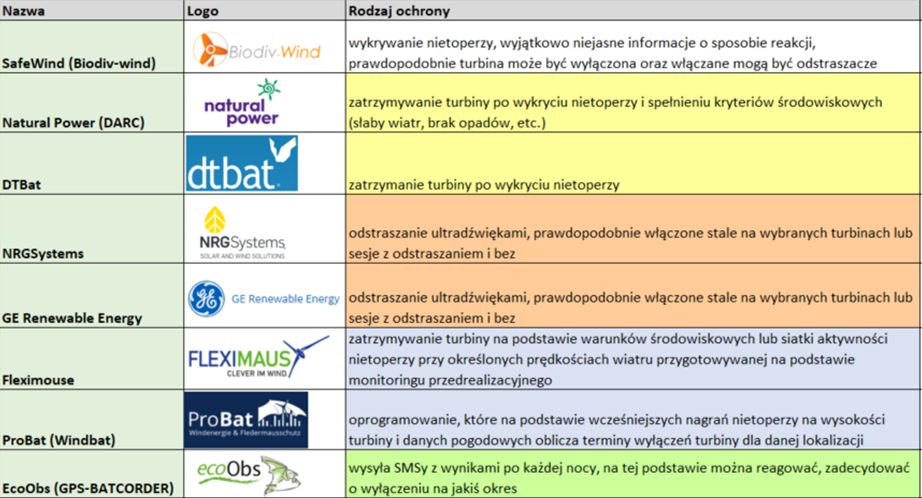
\includegraphics[width=1.0\textwidth]{sprz/konkurencja}
  \caption{Zestawienie i porównanie podobnych rozwiązań.}
  \label{img:konkurencja}
\end{figure} 

\section{IoT}

Mimo, że brak jest jednej definicji tego terminu, i w części publikacji nacisk kładziony jest na różne elementy tego paradygmatu \cite{iot-gov}, bardzo dobrej definicji dostarcza Kavin Ashton, uważany z ojca sformułowania "Internet of Things". Jest to "otwarta i kompleksowa sieć inteligentnych obiektów, które mają zdolność do samoorganizacji, udostępniania informacji, danych i zasobów, reagowania i działania w obliczu sytuacji i zmian w otoczeniu" \cite{Ashton2002}. Definicję tę można uzupełnić tą sformułowaną przez IEEE jako sieć elementów - każdy wyposażony w czujniki - które są podłączone do internetu \cite{IEEE-iot}.

\section{Sieci neuronowe i uczenie głębokie}
Obecnie sieci neuronowe są bardzo ważną częścią świata nowoczesnych technologii i znajdują liczne zastosowania w obszarach automatyzujących wiele procesów takich jak analiza i diagnostyka medyczna \cite{diabetes}, wykrywanie oszustw finansowych \cite{laundring}, rekomendacje sprzedażowe \cite{fashion}, sterowanie procesów przemysłowych \cite{irigation} i wiele innych.

Uczenie głębokie jest podzbiorem sztucznej inteligencji. W procesie uczenia głębokiego posiadając zbiór z odpowiednio zidentyfikowanymi elementami wykonujemy serię nieliniowych przekształceń, tak aby otrzymana funkcja rozdzieliła zbiór niezidentyfikowanych elementów w taki sposób, by w każdej kategorii znalazły się tylko elementy danej klasy.

Struktura matematyczno-programistyczna, służąca do wytworzenia funkcji klasyfikującej elementy zbioru, to właśnie sieć neuronowa. Zamysł konstrukcji sieci neuronowej został zainspirowany budową ludzkiego mózgu. Składa się ona z połączonych ze sobą warstw wielu neuronów. Każdy neuron składa się z wartości początkowej, wagi i funkcji aktywacji, wszystkie te wartości są wartościami matematycznymi. 

\begin{figure}[h]
  \centering
  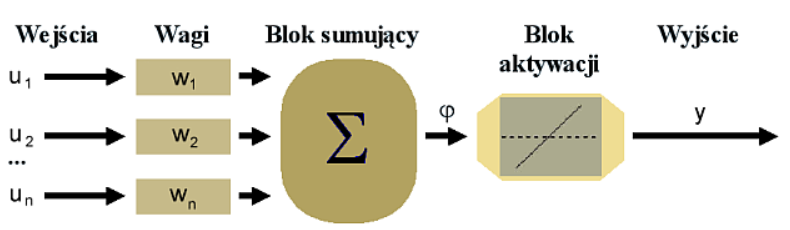
\includegraphics[width=0.8\textwidth]{sprz/neuron}
  \caption{Model neuronu. Źródło: \cite{neuron}}
  \label{img:neuron}
\end{figure} 

\section{Kooperacja z Bioseco S.A.}
Bioseco S.A. jest innowacyjną polską firmą technologiczną z siedzibą w Gdańsku, która opracowała systemy wizyjne wykorzystujące sztuczną inteligencję do ochrony zwierząt, głównie ptaków, na farmach wiatrowych i lotniskach \cite{bioseco1} \cite{bioseco2}. System opracowany i rozwijany jest w kierunku maksymalizacji ochrony zwierząt i minimalizacji strat produkcji. W związku z tym, że aktualnie większość klientów stanowią operatorzy farm wiatrowych, a obok problemu śmiertelności ptaków, drugim najważniejszym przyrodniczym problemem jest śmiertelność nietoperzy \cite{birds-and-bats}, w planach firmy znalazła się również eksploracja tego tematu i możliwość rozwoju technologii do ochrony nietoperzy. Jedna z osób z zespołu inżynierskiego posiada już wiedzę dziedzinową z zakresu zainteresowań Bioseco S.A. Po pomyślnych konsultacjach z firmą przygotowano temat i zakres współpracy spełniający wymogi pracy dyplomowej a jednocześnie zakres zainteresowań przedsiębiorcy.

\chapter{Metody pracy}

\section{Proces wytwórczy}
W trakcie procesu wytwórczego kluczowymi wymaganiami, które powinien spełniać system były: wybrany mikrofon ultradźwięków możliwy do zastosowania na turbinie wiatrowej, zaimplementowane pobieranie nagrań z mikrofonu, identyfikacja gatunków nietoperzy w tych nagraniach, zapis tych informacji do bazy danych oraz wizualizacja ich w interfejsie użytkownika. 

\subsection{Przyjęte podejście}
Zastosowano podejście hybrydowe: Water-Scrum-Fall \cite{water-scrum-fall1} \cite{water-scrum-fall2} \cite{water-scrum-fall3}. Podejście Scrum jest typowe dla projektów, w których ostateczny kształt projektu nie jest znany i jest wymagana duża elastyczność w procesie wytwórczym. Scrum jest więc szczególnie predestynowany do wykorzystania w projektach R\&D, takich jak niniejsza praca inżynierska. Mimo to, z uwagi na duże doświadczenie firmy Bioseco S.A. w pracy z klientami i znajomość ich potrzeb, część wymagań musiała być ściśle określona w początkowej fazie przygotowania systemu, w której wymagania te zdefiniowano, przenalizowano dostępne na rynku zasoby i na tej podstawie przygotowano wstępny projekt systemu. Część wymagań jednak nie była dokładnie zdefiniowana, takich jak np. jaka powinna być architektura rejestratora ultradźwięków, aby realizować zadanie wykrywania nietoperzy na farmach wiatrowych. Do realizacji tego typu wymagań bardzo dobrze nadawało się podejście iteracyjne.

Prace rozpoczęto od przygotowania wymagań systemowych, analiz i wstępnego projektu systemu. 

W kolejnej fazie wytwarzania oprogramowania zastosowano metodę programowania zwinnego w oparciu o plany i dokumentację z pierwszego etapu, korygowane na bieżąco przy każdej iteracji. Przyjęto czas trwania sprintu na cztery tygodnie. Przyjęto tak długi okres sprintu z uwagi na liczbę i skalę potencjalnych zagrożeń oraz obciążeń członków zespołu projektowego, jak również występowanie licznych konsultantów zewnętrznych, których ograniczenia mogły dodatkowo wpływać na wydłużenie prac. 

W ostatniej fazie, po zakończeniu etapu zwinnego, przewidziano testy systemowe i integracyjne. Schemat metodyki wytwarzania oprogramowania przedstawiono poniżej. Odstępstwem od tej wizualizacji było brak elementu "Daily Scrum meeting", który został zastąpiony spotkaniami raz w tygodniu, a w pozostałym czasie komunikacja miała miejsce przez media opisane w rozdziale "Infrastruktura komunikacyjna i dokumentacja". 

\begin{figure}[h]
  \centering
  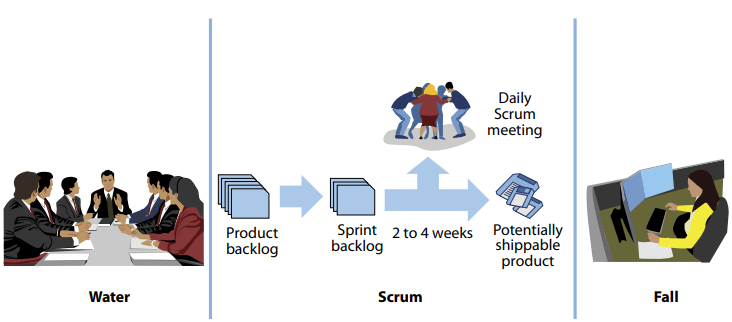
\includegraphics[width=0.8\textwidth]{sprz/water-scrum-fall.png}
  \caption{Graficzna prezentacja metodyki Water-Scrum-Fall. Źródło: \cite{water-scrum-fall1}}
  \label{img:water-scrum-fall}
\end{figure}

\subsection{Przebieg procesu wytwórczego}

\subsubsection{Faza Water}
W fazie "Water" przygotowano wymagania systemowe, wszelkie niezbędne w początkowym etapie analizy oraz wstępny projekt systemu. W tym czasie powstała większość dokumentacji. Był to również okres intensywnych konsultacji z Bioseco S.A. oraz konsultantami dziedzinowymi - Animal Sound Labs, Tribio Sp. z o.o. i dr Joanną Furmankiewicz. Był to też główny okres, w którym trwały prace nad doborem odpowiedniego mikrofonu ultradźwięków, co rzutowało na dalszą konstrukcję całego systemu.

\begin{itemize}
  \item{październik 2022 - spotkanie z Bioseco S.A., odbiór wstępnie dobranego sprzętu do realizacji projektu, zarys wymagań systemowych, wybranie narzędzi komunikacji i metod procesu wytwórczego,}
  \item{listopad 2022 - spotkanie z Bioseco S.A., wstępny dobór technologii, weryfikacja możliwości wykorzystania sprzętu pozyskanego z Bioseco S.A., opracowanie strategii co do pozyskania bądź opracowania nagrań nietoperzy do modelu DL, rozpoczęcie procesu pozyskania nagrań nietoperzy do modelu DL,}
  \item{grudzień 2022 - przygotowanie dokumentacji (Karta Projektu, Dokument Założeń Wstępnych, Specyfikacja Wymagań Systemowych, Rich Picture), weryfikacja możliwości wykorzystania sprzętu pozyskanego z Bioseco S.A. w MVP, wytworzenie sztucznego głosu nietoperza, pozyskanie nagrań nietoperzy do modelu DL,}
  \item{styczeń 2023 - wstępny projekt architektury systemu i przepływu danych między jego elementami, testy otrzymanego z Bioseco S.A. mikrofonu - sprawdzenie poprawności odtwarzania ultradźwięków przez głośnik i poprawności rejestracji przez mikrofon, poszukiwania odpowiedniego mikrofonu ultradźwięków do MVP, pozyskanie nagrań nietoperzy do modelu DL,}
  \item {luty 2023 - wstępny projekt bazy danych, weryfikacja wybranych technologii do implementacji interfejsu użytkownika i bazy danych, poszukiwania odpowiedniego mikrofonu ultradźwięków do MVP.}
  \end{itemize}

\subsubsection{Faza Scrum}
Na podstawie planów i materiałów zgromadzonych w fazie "Water", w fazie "Scrum" wybrano kolejno kilka mikrofonów ultradźwięków możliwych do zastosowania w MVP. Po ostatecznym doborze mikrofonu przygotowano pod kątem sieciowym i fizycznym instalację mikrofonu na turbinie. Po instalacji mikrofonu przeprowadzono testy terenowe wykrywalności ultradźwięków, podsumowano wyniki i na ich podstawie przygotowano propozycję liczby i lokalizacji mikrofonów na turbinie w celu poprawności realizacji zadania ochrony nietoperzy. W tym okresie trwały też intensywne konsultacje z firmą Wildlife Acoustics w sprawie szczegółów montażu mikrofonów oraz z firmą Bioseco S.A. w celu konfiguracji i instalacji systemu SMART. 

Po weryfikacji poprawności działania systemu SMART rozpoczęto implementację pobierania danych z mikrofonu, bazy danych, interfejsu użytkownika, modelu DL oraz przepływu danych pomiędzy tymi elementami.

\begin{itemize}
  \item{marzec 2023 - nauka NodeJS, React, PyTorch i sieci neuronowych, konsultacje z Bioseco S.A. i Animal Sound Labs w sprawie możliwego do zastosowania mikofonu ultradźwięków, wybór mikrofonu możliwego do zastosowania w MVP (mikrofon dostosowany przez firmę Animal Sound Labs wraz z zaprojektowaną przez Animal Sound Labs drogą analogowo-cyfrową, dostosowane do zakresu MVP),}
  \item{kwiecień 2023 - nauka NodeJS, React, PyTorch i sieci neuronowych, konsultacje z Bioseco S.A. i EcoObs w sprawie możliwego do zastosowania mikofonu ultradźwięków, wybór kolejnych mikrofonów możliwych do zastosowania w MVP (Batcorder GSM firmy EcoObs, SMM-U2 firmy Wildlife Acoustics),}
  \item{maj 2023 - nauka NodeJS, React, PyTorch, nauka i konsultacje w sprawie możliwych do wykorzystania architektur sieci neuronowych (z Aleksandrem Obuchowskim), ostateczne wybranie mikrofonu ultradźwięków do MVP (system SMART firmy Wildlife Acoustics), przygotowanie szczegółowego planu testów terenowych mikrofonu (konsultacje z pracownikami Bioseco S.A.) w tym wytworzenie sztucznych głosów nietoperzy,}
  \item{czerwiec 2023 - opracowanie fizycznego i sieciowego podłączenia systemu SMART na turbinie wiatrowej (wraz z pracownikami Bioseco S.A.),}
  \item{lipiec 2023 - konfiguracja sieciowa i podłączenie systemu SMART na turbinie wiatrowej (zrealizowane przez pracowników Bioseco S.A.), kontrola poprawności działania systemu SMART,}
  \item{sierpień 2023 - kontrola poprawności działania systemu SMART, konsultacje z Wildlife Acoustics co do liczby i umiejscowienia mikrofonów na turbinie wiatrowej,}
  \item{wrzesień 2023 - realizacja testów terenowych systemu SMART i opracowanie wyników, konsultacje z Wildlife Acoustics co do liczby i umiejscowienia mikrofonów na turbinie wiatrowej,}
  \item{październik 2023 - dostosowanie architektury systemu do nowo dobranego mikrofonu ultradźwięków, implementacja bazy danych, aplikacji i modelu DL, konsultacje z Wildlife Acoustics co do liczby i umiejscowienia mikrofonów na turbinie wiatrowej, opracowanie pobierania danych z mikrofonu,}
  \item {listopad 2023 - spotkanie z Bioseco S.A. w sprawie możliwego przepływu danych pomiędzy elementami systemu oraz implementacja przepływu danych, implementacja bazy danych, aplikacji, modelu DL i watchdoga, dopracowanie pobierania danych z mikrofonu,}
  \item {grudzień 2023 - implementacja aplikacji, modelu DL i watchdoga.}
  \end{itemize}

\subsubsection{Faza Fall}
Po okresie zwinnym, w fazie "Fall" zweryfikowano poprawność działania systemu i realizowanych przez niego zadań z użyciem testów systemowych i funkcjonalnych.
\begin{itemize}
  \item{styczeń 2024 - testy systemowe i funkcjonalne}
  \end{itemize}

\subsection{Organizacja zespołu}
Grupa inżynierska była samoorganizującym się zespołem. Część funkcji była silniej przypisana do konkretnych członków grupy:
Juliusz Orłowski - Software Developer, Software Engineer, Jakub Prucnal - AI Developer, Software Engineer, Magdalena Wybraniec - Product Owner, Project Manager, specjalista dziedzinowy, AI Developer. 

\section{Środowisko technologiczne}

\subsection{Technologie}
Sprzęt wykorzystany do realizacji ostatecznego rozwiązania to system SMART firmy Wildlife Acoustics. Pozostałe najważniejsze sprzęty wykorzystane do realizacji projektu to głośnik ultradźwiękowy Pettersson L400 i laptop DELL G3. System SMART został wybrany w efekcie długotrwałego procesu doboru mikrofonu przez zespół inżynierski, który opisano w podpunkcie "Mikrofon ultradźwięków spełniający wymogi końcowego produktu". Głośnik ultradźwięków Pettersson L400 został wybrany jako jeden z bardzo nielicznych tego typu sprzętów dostępnych na rynku i został wyprodukowany przez jednego z najważniejszych producentów sprzętów do detekcji nietoperzy oraz głośników ultradźwięków - firmę Pettersson Electronic AB.

Model sieci neuronowej napisany został w języku Python z wykorzystaniem bibliotek PyTorch i TorchAudio.
PyTorch jest biblioteką oferującą narzędzia do budowy i trenowania sieci neuronowych, zawiera m.in. moduły do tworzenia warstw sieci, funkcji straty czy optymalizatorów, daje wsparcie do trenowania na kartach graficznych \cite{pytorch}.
PyTorch jest biblioteką o podobnej popularności co Tensorflow, a w ostatnich latach nawet częściej wykorzystywaną, szczególnie w środowiskach akademickich. Umożliwia ona na większą elastyczność w budowie sieci i ustawieniach jej parametrów. Do zalet takiego rozwiązania należy większy wpływ na kształt i funkcjonowanie sieci, a do wad - dłuższy czas przygotowania oraz wyższy próg wejścia. 

Biblioteka TorchAudio jest częścią ekosystemu PyTorch i służy do obsługi i obróbki plików dźwiękowych. Dostarcza narzędzi pomocnych w ładowaniu danych audio oraz transformacjach takich jak zmiany prędkości czy głośności, przetwarzanie na spektrogramy czy mel-spektrogramy \cite{torchaudio}.

Baza danych została przygotowana w MySQL.

Interfejs użytkownika został napisany w języku JavaScript z użyciem biblioteki ReactJS. Serwer aplikacji został napisany w technologii NodeJS. Użyto również szeregu bibliotek wspomagających tworzenie aplikacji, bazy danych i testów: Sequelize, Express, Jest, Supertest, Joi, Jsonwebtoken. 

MySQL, NodeJS oraz React zostały wykorzystane w znacznej mierze dlatego, że są one używane przez firmę Bioseco S.A. Oznacza to, że poprawnie sprawdzają się w podobnych zastosowaniach oraz w przypadku komercjalizacji produktu, integracja z ekosystemem Bioseco S.A. będzie sprawniejsza niż w przypadku użycia innych technologii.

\subsection{Infrastruktura techniczna}
Na infrastrukturę techniczną, która umożliwiła realizację kluczowych elementów projektu dyplomowego składały się:
\begin{itemize}
  \item{Internet,}
  \item{sieć lokalna LAN firmy Bioseco S.A.,}
  \item{sieć światłowodowa turbiny wiatrowej,}
  \item{sprzęt komputerowy prywatny i służbowy,}
  \item{przęt do rejestracji nietoperzy (mikrofony ultradźwięków oraz system SMART),}
  \item{przęt do odtwarzania głosów nietoperzy (głośnik ultradźwiękowy Pettersson L400),}
  \end{itemize}

\subsection{Infrastruktura komunikacyjna i dokumentacja}
Kominikacja w ramach projektu odbywała się pomiędzy następującymi jednostkami:
\begin{itemize}
  \item{w obrębie grupy,}
  \item{pomiędzy grupą i Promotorem,}
  \item{pomiędzy grupą i Konsultantami.}
  \end{itemize}

Komunikacja w obrębie grupy inżynierskiej oraz pomiędzy grupą i Konsultantami z Bioseco S.A. i pozostałymi specjalistami odbywała się z wykorzystaniem wielu mediów:
\begin{itemize}
  \item{osobiście - spotkania w ramach zajęć na Uczelni,}
  \item{osobiście - spotkania poza zajęciami na Uczelni,}
  \item{osobiście - spotkania w ramach konsultacji,}
  \item{osobiście - spotkania w ramach pracy w Bioseco S.A.,}
  \item{aplikację Teams,}
  \item{aplikację Zoom,}
  \item{aplikację ClickUp,}
  \item{grupę w aplikacji WhatsApp,}
  \item{mailowo poprzez maile uczelniane, prywatne i służbowe}
  \item{telefonicznie.}
  \end{itemize}

Komunikacja pomiędzy grupą inżynierską a Promotorem odbywała się poprzez następujące media:
\begin{itemize}
  \item{osobiście - spotkania w ramach zajęć na Uczelni,}
  \item{aplikację Teams,}
  \item{mailowo poprzez maile uczelniane.}
  \end{itemize}

Dokumentacja prowadzona była w:
\begin{itemize}
  \item{repozytorium na GitHub,}
  \item{aplikacji Teams,}
  \item{aplikacji ClickUp.}
  \end{itemize}

\section{Analiza zagrożeń}

Do głównych zagrożeń projektu należą \textit{de facto} te związane z ograniczonymi zasobami czasowymi oraz ograniczoną wiedzą i doświadczeniem. Pozostają jeszcze zagrożenie losowe, takie jak np. choroby, które jeśli wystąpią mogą sprawić, że możliwość realizacji projektu zmieni się diametralnie.

\begin{figure}[h]
  \centering
  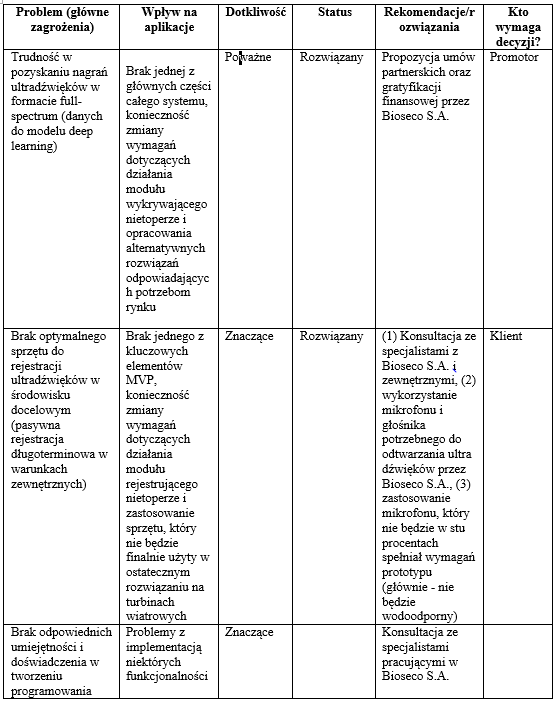
\includegraphics[width=1.0\textwidth]{sprz/sodis1.png}
  \caption{Analiza zagrożeń w konwencji soDIS}
  \label{img:sodis1}
\end{figure}

\begin{figure}[h]
  \centering
  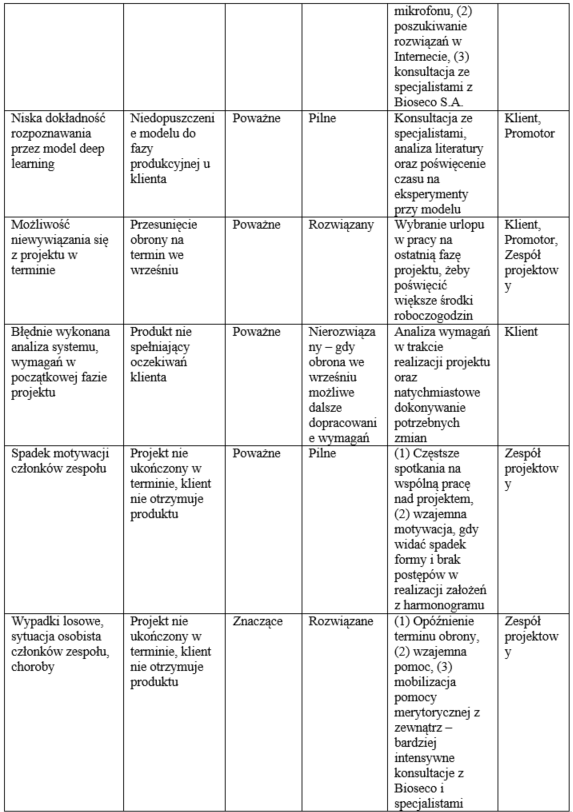
\includegraphics[width=1.0\textwidth]{sprz/sodis2.png}
  \caption{Analiza zagrożeń w konwencji soDIS}
  \label{img:sodis2}
\end{figure}

\subsection{Wpływ na realizację projektu}
Wpływ zagrożeń opisanych w niniejszym dokumencie jest potencjalnie wysoki, dlatego że projekt jest rozbudowany, innowacyjny, i powstaje na studiach zaocznych, w związku z czym zespół projektowy obłożony jest znaczną ilością dodatkowych obowiązków pozaszkolnych, a także pozbawiony jest dużego doświadczenia w realizacji tego typu projektów.

\subsection{Rekomendacje i rozwiązania}
Podsumowaniem szczegółowych rekomendacji umieszczonych w tabeli - "Analiza zagrożeń w konwencji soDIS - są zwłaszcza konsultacje ze specjalistami w wybranych dziedzinach i pomoc ze strony Bioseco S.A.,  w szczególności w rozmowach partnerskich związanych z pozyskaniem nagrań nietoperzy oraz zapewnieniu nowego sprzętu do eksperymentów. Ponadto kluczowymi zaleceniami do minimalizacji zagrożeń są: ciągła weryfikacja wymagań na system, wzajemne wsparcie i wsparcie bliskich oraz sport.

\chapter{Prace badawcze - projektowanie}

Przygotowanie całości projektu składało się z zaprojektowania prac badawczych, realizacji tych prac oraz wdrożenia systemu składającego się z mikrofonu ultradźwięków pobierającego dane z otoczenia, kolejno przekazywane do modelu DL analizującego dźwięk pod kątem występowania gatunku nietoperza i zapisującego te dane w bazie danych i wizualizujących w aplikacji użytkownika. Struktura systemu została ustalona przez Bioseco S.A. oraz Promotora pracy, a jej ostateczny kształt jest rezultatem eksperymentów. 

\section{Konsultacje z Bioseco S.A.}
W ramach kooperacji z Bioseco S.A. przeprowadzono spotkania wspomagające zespół inżynierski w procesie wytwórczym, udostępniono większość niezbędnego sprzętu oraz wiedzę z zakresu prowadzenia badań terenowych i opracowania danych, wytwarzania oprogramowania i działania dedykowanych sprzętów. Zrealizowano konfigurację sieciową udostępnionego sprzętu, tak aby umożliwić zdalny dostęp do danych z mikrofonu ultradźwięków. Zainstalowano również testowo mikrofon ultradźwięków na turbinie wiatrowej.

\section{Wymagania}
  
W niniejszym podrozdziale wymienia i opisuje się wymagania narzucone przez klienta - Bioseco S.A., przedstawicieli Uczelni – Dziekana i Promotora, a także przez aktualne standardy prawne dotyczące ochrony przyrody oraz aktualne standardy sprzętowe dotyczące nagrywania i identyfikacji nietoperzy.

\subsection*{Wymagania ogólne i dziedzinowe}

  \begin{requirementstab}[label={tab:requirements:general},caption={Baza danych nagrań głosów nietoperzy}]
    \id{WO 01}
    \priority{M}
    \name{Baza danych nagrań głosów nietoperzy}
    \descr{Zebranie lub pozyskanie bazy danych głosów nietoperzy oraz jej przygotowanie, która posłuży do stworzenia modelu rozpoznawania wystąpienia nietoperza i/lub gatunku nietoperza.}
    \sholder{UOB 01, UOP 01, UNB 01}
    \reqrelated{WO 03}
  \end{requirementstab}

  \begin{requirementstab}[label={tab:requirements:general},caption={Ekologia}]
    \id{WO 02}
    \priority{M}
    \name{Ekologia}
    \descr{System ma chronić nietoperze przed szkodliwym działaniem farm wiatrowych na ich populację}
    \sholder{UNB 01, UNP 01, UNP 02}
    \reqrelated{WO 03}
  \end{requirementstab}
    
  \begin{requirementstab}[label={tab:requirements:general},caption={Normy prawa}]
    \id{WO 03}
    \priority{M}
    \name{Normy prawa ochrony przyrody i prawa dotyczącego ocen oddziaływania na środowisko}
    \descr{System poprzez swoją przyszłą funkcjonalność wyłączania turbiny będzie stanowił alternatywę dla jedynego obecnie rodzaju działań minimalizujących wpływ turbin na nietoperze, czyli 3 lat monitoringu porealizacyjnego i adekwatnych do jego wyników, narzuconych z góry okresowych wyłączeń turbin, co przyniesie znaczne oszczędności dla deweloperów farm wiatrowych.}
    \sholder{UNP 02}
    \reqrelated{WO 02}
  \end{requirementstab}

  \begin{requirementstab}[label={tab:requirements:general},caption={System rozpoznawania gatunków nietoperzy}]
    \id{WO 04}
    \priority{S}
    \name{System rozpoznawania gatunków nietoperzy}
    \descr{System do rozpoznawania gatunków nietoperzy jest kosztowny, stworzenie go będzie oprogramowaniem, który przyniesie dodatkowe zyski.}
    \sholder{UOB 01, UNB01}
    \reqrelated{}
  \end{requirementstab}
  
  \clearpage

\subsection*{Wymagania funkcjonalne}

  \begin{requirementstab}[label={tab:requirements:func1},caption={System rozpoznawania wystąpienia nietoperza}]
    \id{WF02}
    \priority{M}
    \name{System rozpoznawania wystąpienia nietoperza}
    \descr{Opracowanie algorytmu uczenia maszynowego oraz rozpoznawania wystąpienia nietoperza na żywo poprzez śledzenie sygnałów uzyskanych za pomocą urządzenia do detekcji.}
    \acceptcrit{Wytrenowany model do rozpoznawania wystąpienia nietoperzy.}
    \inputdata{Zbiór nagrań ultradźwięków nietoperzy} 
    \postconditions{Wytrenowany model}
    \implementation{}
    \sholder{UNB 01, UNP 01}
    \reqrelated{}
  \end{requirementstab}

  \begin{requirementstab}[label={tab:requirements:func1},caption={System uczenia sieci neuronowej}]
    \id{WF03}
    \priority{C}
    \name{System uczenia sieci neuronowej}
    \descr{Opracowanie systemu do uczenia sieci neuronowej rozpoznawania gatunków nietoperzy.}
    \acceptcrit{Stworzony algorytm do tworzenia modelu do rozpoznawania gatunku nietoperza}
    \inputdata{Zbiór nagrań ultradźwięków nietoperzy}
    \postconditions{Wytrenowany model}
    \implementation{}
    \sholder{UOB 01, UOP 01}
    \reqrelated{}
  \end{requirementstab}

  \begin{requirementstab}[label={tab:requirements:func1},caption={System rozpoznawania gatunku nietoperza}]
    \id{WF04}
    \priority{S}
    \name{System rozpoznawania gatunku nietoperza}
    \descr{Opracowanie systemu do rozpoznawania gatunku nietoperza za pomocą detektora.}
    \acceptcrit{Stworzenie modelu oraz połączenie go z urządzeniem do rozpoznawania nietoperzy.}
    \inputdata{Zbiór nagrań ultradźwięków nietoperzy}
    \postconditions{Wytrenowany model}
    \implementation{}
    \sholder{UOB 01}
    \reqrelated{}
  \end{requirementstab}

  \begin{requirementstab}[label={tab:requirements:func1},caption={Interfejs do wizualizacji danych}]
    \id{WF05}
    \priority{M}
    \name{Interfejs do wizualizacji danych}
    \descr{Stworzenie interfejsu do przeglądania danych pobieranych z bazy danych i wizualizacja tych danych.}
    \acceptcrit{Stworzony interfejs działający i spełniający swoją funkcję.}
    \inputdata{Nagrania pochodzące z mikrofonu ultradźwięków}
    \postconditions{Nagrania widoczne w interfejsie użytkownika}
    \implementation{}
    \sholder{UOB 01}
    \reqrelated{}
  \end{requirementstab}

  \begin{requirementstab}[label={tab:requirements:func1},caption={Liczba i lokalizacja mikrofonów na turbinie}]
    \id{WF06}
    \priority{M}
    \name{Pokrycie kąta 360 stopni dookoła turbiny poprzez rejestrację ultradźwiękową}
    \descr{Plan liczby i lokalizacji mikrofonów ultradźwięków na turbinie wiatrowej tak, aby system pełnił funkcję ochrony nietoperzy}
    \acceptcrit{Realizacja testów terenowych mikrofonu}
    \inputdata{Mikrofon ultradźwięków}
    \postconditions{Pokrycie kąta 360\textdegree przez rejestrację ultradźwękową}
    \implementation{}
    \sholder{UOP 01, UNB 01}
    \reqrelated{}
  \end{requirementstab}
  
  \clearpage

\subsection*{Interfejs z otoczeniem}
  
  \begin{requirementstab}[label={tab:requirements:func1},caption={System wyłączający wiatraki}]
    \id{WF01}
    \priority{M}
    \name{System wyłączający wiatraki}
    \descr{Połączenie systemu wykrycia nietoperza z systemem wyłączającym wiatraki}
    \acceptcrit{Stworzenie punktu styku, który będzie jako output dawać sygnał do systemu wyłączającego wiatraki.}
    \inputdata{Zidentyfikowane nagrania nietoperzy}
    \postconditions{Wystawione API z informacją o konieczności wyłączenia turbiny}
    \implementation{}
    \sholder{UNB 01, UNP 01}
    \reqrelated{}
  \end{requirementstab}

  \begin{requirementstab}[label={tab:requirements:func1},caption={Baza danych}]
    \id{WF02}
    \priority{M}
    \name{Baza danych}
    \descr{Połączenie systemu z bazą danych, która będzie zbierać dane wystąpienia nietoperza}
    \acceptcrit{Stworzenie punktu styku, który będzie jako output dawać sygnał do systemu wyłączającego wiatraki.}
    \inputdata{Nagrania nietoperzy z mikrofonu ultradźwięków}
    \postconditions{Nagrania zapisane w bazie danych}
    \implementation{}
    \sholder{UOP 01, UNB 01}
    \reqrelated{}
  \end{requirementstab}

  \clearpage

\section{Konsultacje chiropterologiczne i detektorowe}
W początkowej fazie przygotowania projektu przeprowadzono konsultacje chiropterologiczne obejmujące: pozyskanie zidentyfikowanych nagrań nietoperzy, typu nagrań jakich należy użyć do uczenia głębokiego, rodzaju rejestratorów ultradźwięków jakie mogą być wykorzystane na turbinie wiatrowej w rozwiązaniu końcowym. Konsultacje te przeprowadzono z najlepszymi polskimi chiropterologami oraz polskim, niemieckim i amerykańskim wytwórcą detektorów. Chiropterolodzy, z którymi przeprowadzono konsultacje to: Aneta Zapart, Konrad Bidziński (z Tribio Sp. z o.o.) i dr Joanna Furmankiewicz. Firmy wytwarzające detektory, z którymi prowadzono konsultacje to: Animal Sound Labs, EcoObs, Wildlife Acoustics.

\section{Mikrofon ultradźwięków spełniający wymogi końcowego produktu}
W procesie definiowania cech sprzętu jakie powinien posiadać mikrofon i rejestrator ultradźwięków wyszczególniono następujące cechy:
  \begin{itemize}
    \item{możliwie najwyższa jakość rejestrowanych ultradźwięków,}
    \item{możliwie największa odległość rejestrowanych ultradźwięków,}
    \item{wodoodporność,}
    \item{możliwość sprzętowa do integracji ze sprzętem i oprogramowaniem umożliwiającym pobieranie danych w czasie rzeczywistym.}
  \end{itemize}

W początkowym okresie prac nad systemem nie istniał mikrofon spełniające wszystkie powyższe kryteria. W mikrofonie otrzymanym początkowo z Bioseco S.A. brakowało wodoodporności. W detektorze Batcorder firmy EcoObs i mikrofonie SMM-U2 Wildlife Acoustics brakowało bezpośredniej możliwości podłączenia do urządzenia typu Raspberry Pi i nieograniczonego dostępu do danych. Wykonano próby współpracy z Animal Sound Labs, podczas których używając dostępnych najlepszych mikrofonów posiadanych przez firmę oraz projektując odpowiednią drogę analogowo-cyfrową z możliwością połączenia przez USB do urządzenia typu Raspberry Pi miał powstać odpowiedni mikrofon, jednak próby te zakończyły się niepowodzeniem z uwagi na ograniczenia czasowe Animal Sound Labs w zaproponowanym terminie. 

Animal Sound Labs jest polską firmą zajmująca się wytwarzaniem detektorów ultradźwięków. Właściciel firmy - Paweł Federowicz posiada bardzo dużą wiedzę dziedzinową z tego zakresu, dlatego bardzo szybko rozpoczęto z nim rozległe konsultacje dotyczące części projektu inżynierskiego związanego z doborem mikrofonu ultradźwięków oraz przetwarzaniem sygnałów. W trakcie rozmów pomiędzy Bioseco S.A. i Animal Sound Labs dopracowano zakres prac ze strony Animal Sound Labs jaki opisano powyżej. Z uwagi jednak na fakt niewielkiej liczby pracowników oraz znaczne obciążenie Animal Sound Labs w tamtym okresie, koopercja nie została zrealizowana.

W tym czasie na rynku pojawiło się nowe urządzenie firmy Wildlife Acoustics - system SMART, który dostarczył wszystkich niezbędnych elementów, jakie wymagane były od sprzętu do realizacji niniejszej pracy dyplomowej (\ref{img:smart}). Na poniższym obrazku przedstawiony jest system SMART - dwa mikrofony ultradźwięków po lewej i prawej stronie oraz kontroler w centrum.

\begin{figure}[h]
  \centering
  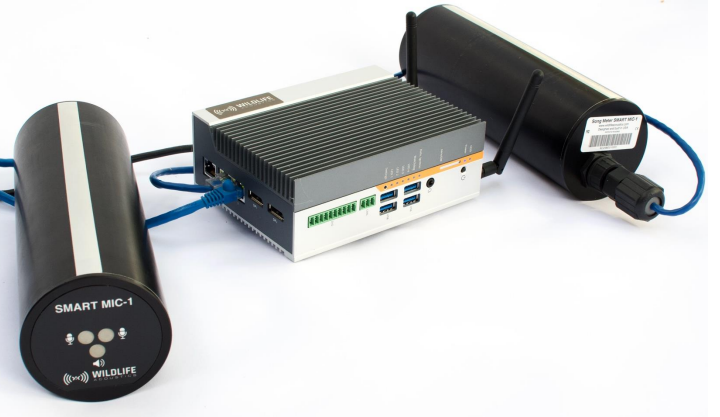
\includegraphics[width=0.8\textwidth]{sprz/smart.png}
  \caption{System SMART firmy Wildlife Acoustics. Źródło: Wildlife Acoustics}
  \label{img:smart}
\end{figure} 

Z korzyścią dla ochrony nietoperzy i deweloperów farm wiatrowych, a z pewnymi zagrożeniami dla twórców niniejszej pracy dyplomowej mikrofon został wyprodukowany wraz z tzw. kontrolerem (prostym przemysłowym komputerem), który wyposażony jest w oprogramowanie pobierające dane z mikrofonu i po odpowiedniej konfiguracji sieciowej serwujący dane i prezentujący je w interfejsie użytkownika \cite{smart-user-guide}. Mimo tego, że całe rozwiązanie częściowo odpowiada zakresowi niniejszej pracy dyplomowej, nie jest ono idealne, np. nie posiada bazy danych czy też w dość znacznym stopniu niepoprawnie identyfikuje gatunki nietoperzy \cite{kaleidoscope-bias}. Mimo to, fakt pracy członków zespołu nad podobnym rozwiązaniem, z uwagi na obszerne zajęcie się takim tematem i wdrożenie się w wiele jego aspektów, niesie raczej możliwości i szanse rozwoju tego rozwiązania, niż zagrożenie ze strony konkurencji.

\section{Odtwarzanie ultradźwięków}
Do wyemitowania ultradźwięków niezbędne są urządzenia obsługujące co najmniej dwukrotnie wyższą częstotliwość niż emitowane dźwięki. Wynika to z twierdzenia Nyquista-Shannona, zgodnie z którym częstotliwość próbkowania z sygnału ciągłego ("analogowego") na dyskretny ("cyfrowy") musi być co najmniej dwukrotnie wyższa od najwyższej składowej widma sygnału aby sygnał został odtworzony poprawnie i nie dochodziło do zjawiska aliasingu \cite{probkowanie}. W zależności od możliwości karty dźwiękowej w komputerze użytym jako generator ultradźwięków, należy bądź ustawić maksymalną wartość próbkowania karty, bądź podłączyć wzmacniacz zwiększający maksymalną częstotliwość odtwarzania.

Do wstępnych testów poprawności działania sprzętu użyto wzmacniacza iFi Zen Dac o maksymalnej częstotliwości odtwarzania 384 kHz, a do testów terenowych mikrofonu - laptopa DELL G3 z maksymalną częstotliwością próbkowania karty dźwiękowej ustawioną na 96 kHz.

\section{Głosy nietoperzy typu full-spectrum}
Dźwięk typu full-spectrum, to rodzaj nagrania i analizy spektralnej dźwięku, w którym ujęte jest pełne spektrum nagrywanych częstotliwości \cite{fullspectrum}. Nagranie tego typu przedstawiono po lewej stronie na poniższym rysunku. W odróżnieniu np. od nagrań typu zero-crossing (po prawej stronie) posiadają dużo więcej informacji o dźwięku, co przedstawiono na ilustracji (\ref{img:fullspectrum}). W przypadku nagrań typu zero-crossing z sygnału wybierane są jedynie punkty, które znajdują się w miejscu przecięcia osi X i Y wykresu sygnału. Tym samym w przypadku nagrań typu zero-crossing wybrana jest około jedna tysięczna sygnału, co pozwala na zmniejszenie rozmiaru nagrań ale również znaczne zmniejszenie ilości informacji o sygnale \cite{fullspectrum}. Z tego powodu nagrania typu full-spectrum są najlepsze do analizy gatunków nietoperzy, a wykorzystanie tego typu nagrań może dać najlepsze efekty w treningu sieci neuronowej oraz predykcji gatunków.

Tego typu nagrania generowane są tylko przez część detektorów ultradźwięków - tylko przez najnowocześniejsze rekordery, co wpłynęło na zmniejszenie liczby potencjalnych źródeł nagrań do treningu sieni neuronowej.

\begin{figure}[h]
  \centering
  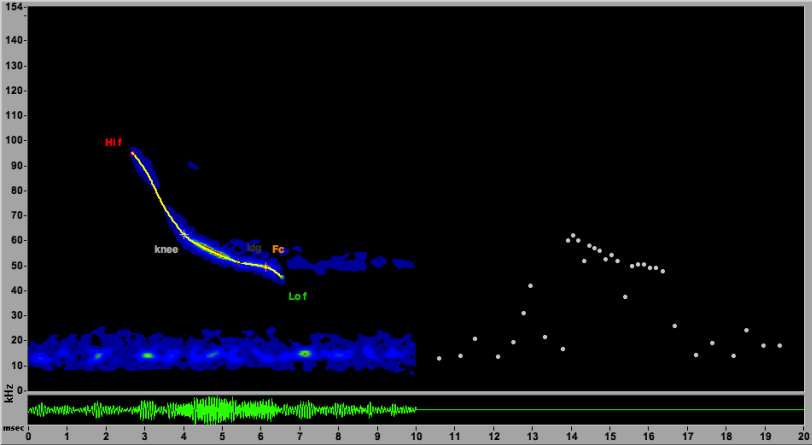
\includegraphics[width=0.8\textwidth]{sprz/fullspectrum.png}
  \caption{Porównanie dźwięku typu full-spectrum (po lewej) z dźwiękiem typu zero-crossing (po prawej). Źródło: \cite{fullspectrum}}
  \label{img:fullspectrum}
\end{figure} 

\subsection{Wytworzenie sztucznych głosów nietoperzy do wstępnych testów sprzętu}

W celu przetestowania działania sprzętu rejestrującego i oprogramowania przetwarzającego zarejestrowane dźwięki, przeprowadzono doświadczenie polegające na sztucznym wytworzeniu dźwięków, które imitowały by głos nietoperza.
Pierwszym etapem było wygenerowanie w programie Audacity sinusoidalnej fali dźwiękowej z początkową częstotliwością 51 kHz i końcową częstotliwością 42 kHz, amplitudą początkową 0 i amplitudą końcową 1, interpolacją logarytmiczną oraz czasem trwania 25 ms. Na poniższym rysunku przedstawiono efekt takiej operacji (\ref{img:wykres_fali}).

\begin{figure}[h]
    \centering
    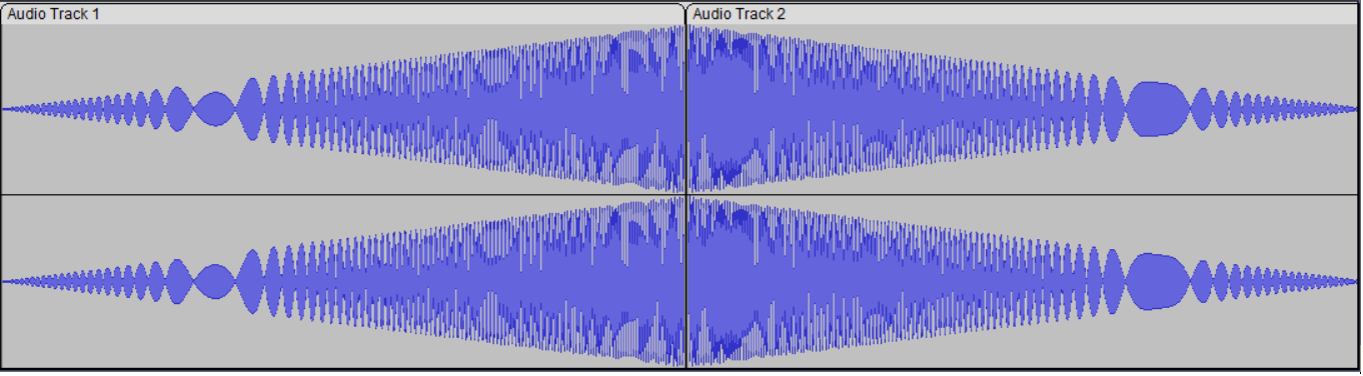
\includegraphics[width=0.8\textwidth]{sprz/wykres_fali}
    \caption{Wykres fali dźwiękowej}
    \label{img:wykres_fali}
\end{figure}

Uzyskany w ten sposób wykres fali dźwiękowej skopiowano dziesięciokrotnie i utworzono sekwencję 500 ms dźwięków, przed którą i po której wprowadzono 500 ms ciszy w celu łatwiejszego wyodrębnienia dźwięków po ich późniejszym zarejestrowaniu. Na poniższym rysunku przedstawiono efekt takiej operacji (\ref{img:wykres_fali_wielokrotnej}).

\begin{figure}[h]
    \centering
    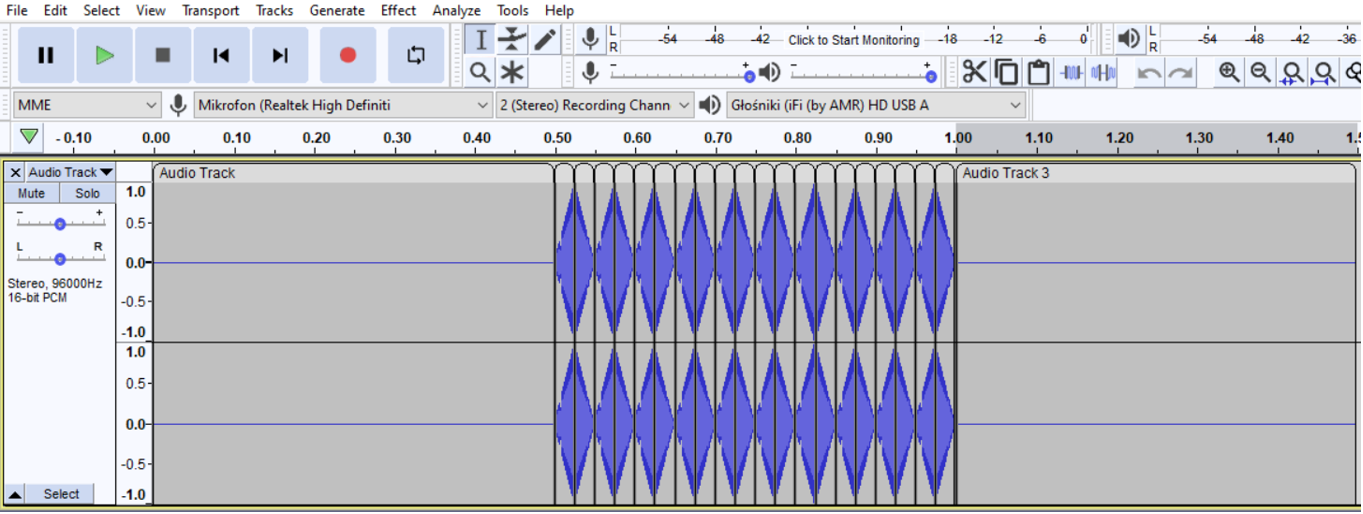
\includegraphics[width=0.8\textwidth]{sprz/wykres_fali_wielokrotnej}
    \caption{Zwielokrotniony wykres fali}
    \label{img:wykres_fali_wielokrotnej}
\end{figure}

Następnie, do wyemitowania dźwięku niezbędne były urządzenia obsługujące co najmniej dwukrotnie wyższą częstotliwość niż emitowane dźwięki. W tym celu do komputera służącego jako generator dźwięku podłączono wzmacniacz iFi Zen Dac o maksymalnej częstotliwości odtwarzania 384 kHz oraz głośnik ultradźwiękowy Pettersson L400 (10-110 kHz). Do zarejestrowania wyemitowanego dźwięku posłużył mikrofon Pettersson M500-384 o częstotliwości próbkowania 384 kHz.

Program BatSound dołączony do mikrofonu posłużył do wizualizacji zarejestrowanego dźwięku (\ref{img:batsound}). W górnej części nagrania dźwięk zobrazowany jest w postaci czasowej, a w dolnej w postaci spektrogramu.

\begin{figure}[h]
    \centering
    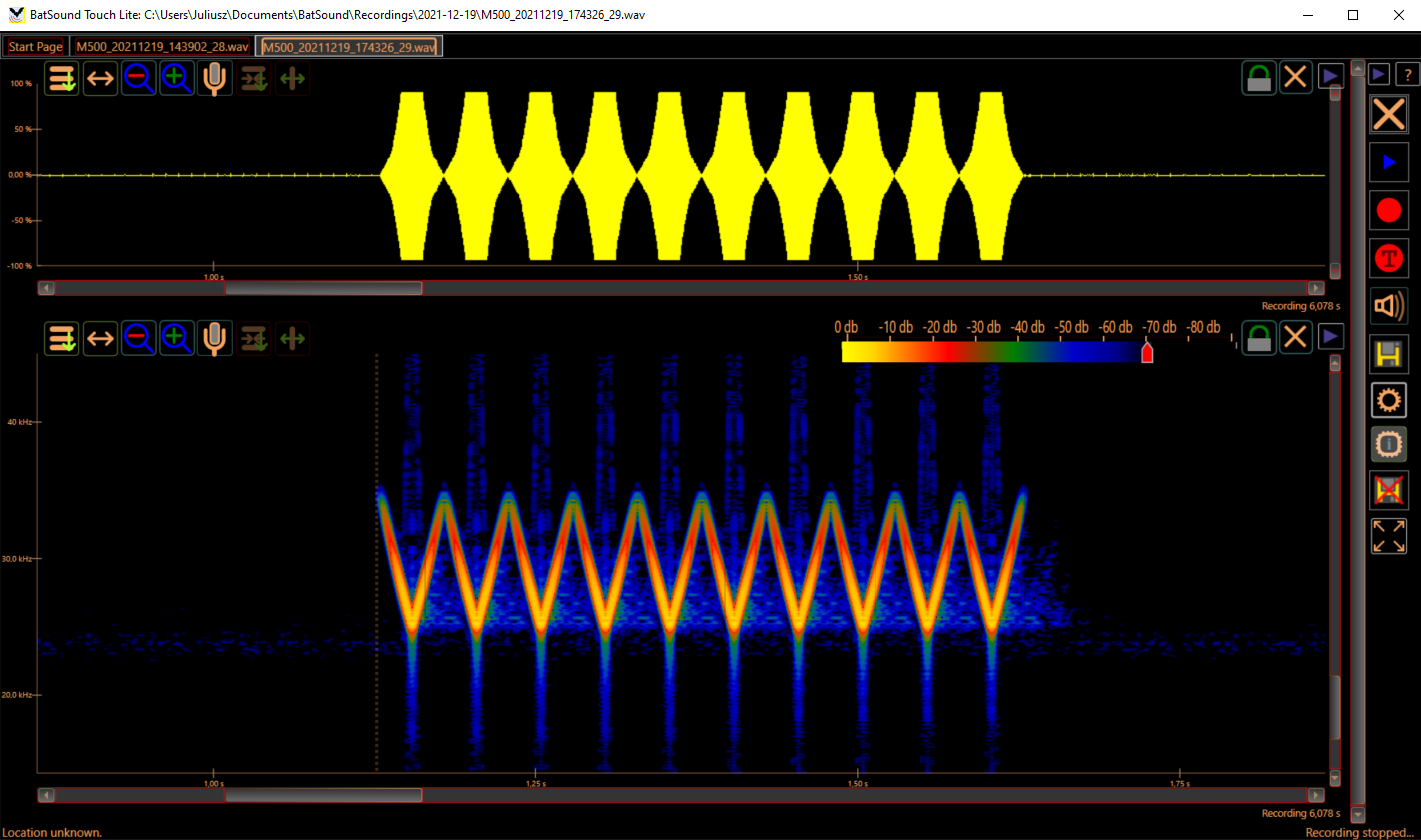
\includegraphics[width=0.8\textwidth]{sprz/batsound}
    \caption{Wykres zarejestrowanego dźwięku zwizualizowany w programie Batsound}
    \label{img:batsound}
\end{figure}

Powyższe doświadczenie dowiodło, iż mikrofon Pettersson M500-384 spełnia swoje zadanie. Mikrofon rejestruje dźwięki w zakresie niesłyszalnym dla człowieka i poprawnie wizualizuje zarejestrowane nagranie.

\subsection{Wytworzenie sztucznych głosów nietoperzy do testów terenowych mikrofonu}
W identyczny sposób jak głosy nietoperzy do wstępnych testów sprzętu przygotowano też dźwięki do testów terenowych. Dźwięki miały częstotliwości: 16-20 kHz, 25-35 kHz, 37-40 kHz i 40-48 kHz. Poszczególne dźwięki zostały zaprojektowane tak, aby reprezentować zakresy częstotliwości najczęściej występujących grup nietoperzy \cite{sachanowicz}, \cite{sachanowicz2}, a jednocześnie nie nakładały się na siebie – dzięki czemu można je było łatwo rozróżnić w wynikach. Poszczególne zakresy częstotliwości odpowiadają następującym gatunkom:

\begin{itemize}
  \item{16-20 kHz – borowiec, borowiaczek,}
  \item{25-35 kHz – mroczek posrebrzany, mroczek późny, mroczek pozłocisty i kilka gatunków z rodzaju Myotis,}
  \item{37-40 kHz – karlik większy i kilka gatunków z rodzaju Myotis,}
  \item{40-48 kHz – karlik większy i karlik malutki.}
\end{itemize}

Większość z tych nietoperzy to gatunki szczególnie narażone na kolizje z turbinami wiatrowymi, to jest: borowiec, borowiaczek, karliki czy mroczek posrebrzany \cite{Wytyczne}, \cite{rodrigues}.

Poniżej przedstawiono zdjęcia borowca (\ref{img:Nyctalus_noctula}) i karlika większego (\ref{img:Pipistrellus_nathusii}) - jednych z dwóch najczęstszych ofiar kolizji z turbinami wiatrowymi.
\begin{figure}[h]
  \centering
  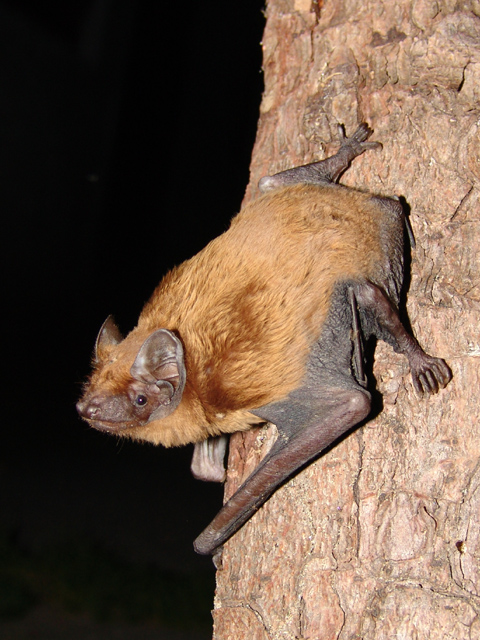
\includegraphics[width=0.5\textwidth]{sprz/Nyctalus_noctula.jpg}
  \caption{Borowiec wielki. Źródło: Wikipedia \cite{wiki-borowiec}}. 
  \label{img:Nyctalus_noctula}
\end{figure} 

\begin{figure}[h]
  \centering
  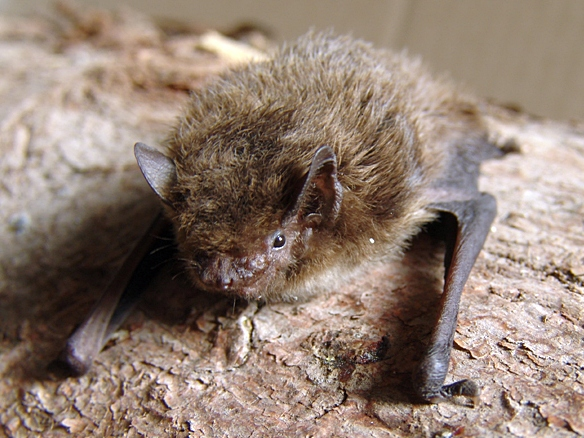
\includegraphics[width=0.5\textwidth]{sprz/Pipistrellus_nathusii.jpg}
  \caption{Karlik większy. Źródło: Wikipedia \cite{wiki-borowiec}}. 
  \label{img:Pipistrellus_nathusii}
\end{figure}

\subsection{Zebranie nagrań nietoperzy}
Zebranie nagrań nietoperzy odpowiedniego typu i odpowiedniej ich liczby rodziło kilka problemów:
\begin{itemize}
  \item{nagrania typu full-spectrum pochodzą z najnowocześniejszych detektorów, które nie są używane przez wszystkich chiropterologów, więc ogranicza to grupę osób posiadających takie nagrania,}
  \item{nagrania powinny pochodzić ze środowiska podobnego do lokalizacji turbin wiatrowych, najlepiej z turbiny wiatrowej z uwagi na podobne składy gatunkowe nietoperzy jakie napotykane będę przez urządzenie po wdrożeniu, a więc powinny pochodzić z monitoringu porealizacyjnego, który prowadzony jest w Polsce przez niewielką grupę chiropterologów, co zmniejsza liczbę osób posiadających takie nagrania}
  \item{nagrań musi być możliwie dużo, do celów skutecznego treningu sieci neuronowej}
  \item{kwestie związane z własnością, potencjalne koszty i związane z tym negocjacje.}
\end{itemize}

Po trwających kilka miesięcy poszukiwaniach osób mogących udostępnić takie nagrania, negocjacjach warunków przekazania nagrań oraz samym procesie przekazywania nagrań, udało się pozyskać 71,7 GB danych, w tym 18 412 nagrań zawierających odgłosy nietoperzy oraz inne dźwięki, takie jak szumy pochodzące z otoczenia. Nagrania przekazała firma Tribio Sp. z o.o. Członkowie zespołu inżynierskiego ogromnie dziękują za tę pomoc, bez której realizacja niniejszej pracy dyplomowej nie byłaby możliwa.

\chapter{Prace badawcze - testy terenowe}

\section{Montaż systemu SMART na turbinie wiatrowej}
System SMART firmy Wildlife Acoustics został zainstalowany na jednej z farm wiatrowych, na których operuje firma Bioseco S.A. przez pracowników firmy. Instalacja miała miejsce 14 lipca 2023. 
 

\section{Konfiguracja sieciowa}
Konfiguracja sieciowa systemu SMART została zrealizowana przez Bioseco S.A.. SMART został połączony poprzez Ethernet do skrzynki zasilająco-sieciowej Bioseco S.A. zainstalowanej w turbinie wiatrowej, poprzez którą system podłączony jest światłowodem do Internetu. Port sieciowy udostępniony z turbiny skonfigurowany jest w taki sposób, aby poprzez VPN w sieci Bioseco S.A. możliwy był dostęp do danych z mikrofonu.

\section{Konsultacje z Wildlife Acoustics}
Konsultacje z firmą Wildlife Acoustics obejmowały takie elementy jak:
\begin{itemize}
  \item{lokalizacja mikrofonu na turbinie wiatrowej (wieża/gondola),}
  \item{lokalizacja kontrolera na turbinie wiatrowej (wieża/gondola),}
  \item{liczba mikrofonów,}
  \item{sposób montażu.}
\end{itemize}

W celu poprawnego zaadresowania powyższych elementów należało uwzględnić następujące aspekty:

\begin{itemize}
  \item{wysokość przelotów nietoperzy, których dotyczy problem śmiertelności,}
  \item{możliwości technologiczne sprzętu, np. najdłuższa możliwa długość kabla Ethernet łączącego mikrofon z kontrolerem,}
  \item{możliwość wytwarzania echa przez elementy turbiny bądź w wyniku nieprawidłowego montażu mikrofonu, co może powodować nieprawidłowości w rejestracji głosów nietoperzy,}
  \item{możliwość lokalizacji sprzętu w turbinie z punktu widzenia deweloperów farm wiatrowych, np. problem lokalizacji źródła zasilania w gondoli,}
  \item {możliwości technologiczne montażu w różnych częściach turbiny i problem dostępu do sprzętu w przypadku jego konserwacji czy naprawy,}
  \item {występowanie bądź nie zaleceń władz środowiskowych co do szczegółów montażu podobnych urządzeń na farmach wiatrowych.}
\end{itemize}

Kluczowe ustalenia z konsultacji są następujące:
\begin{itemize}
  \item{lokalizacja mikrofonu na turbinie wiatrowej najlepiej jeśli będzie w gondoli, ale może być również u podstawy wieży,}
  \item{zaleca się stosowanie dwóch mikrofonów na jednej turbinie, ale możliwy jest montaż jednego mikrofonu, bądź większej ich liczby,}
  \item{z uwagi na ograniczenia w długości kabla Ethernet, który łączy mikrofon z kontrolerem (do 100 m) oraz fakt, że nowoczesne turbiny wiatrowe posiadają wieże wyższe niż 100 m, mikrofon razem z kontrolerem powinny znajdować się albo w gondoli albo na dole wieży turbiny,}
  \item{możliwy jest montaż poprzez umieszczenie mikrofonu w otworze wywierconym w gondoli bądź na szczycie gondoli zamocowany do zewnętrznych elementów gondoli.}
\end{itemize}

\section{Metodyka testów}
Sztucznie przygotowane dźwięki emitowano w kilku konfiguracjach, składających się z różnych odległości, kątów względem mikrofonu i częstotliwości. Dźwięki o częstotliwościach: 16-20 kHz, 25-35 kHz, 37-40 kHz i 40-48 kHz odtwarzane były w odległościach 7, 20, 40, 60, 80, 100 i 120 m od mikrofonu. Dźwięki odtwarzane były w czterech liniach przebiegających pod kątami 0, 30, 60 i 90 stopni w stosunku do przodu mikrofonu (\ref{img:angles}). Dźwięki odtwarzane były z zestawu głośnika ultradźwiękowego Pettersson L400 oraz laptopa z kartą dźwiękową w konfiguracji umożliwiającej odtwarzanie dźwięków o wysokiej częstotliwości (16-bit, 48 kHz). Dźwięki odtwarzane były w możliwie najwyższym natężeniu. Każdy dźwięk był emitowany w określonej odległości i pod określonym kątem od trzech do sześciu razy, w większości przypadków trzy razy.

\begin{figure}[h]
  \centering
  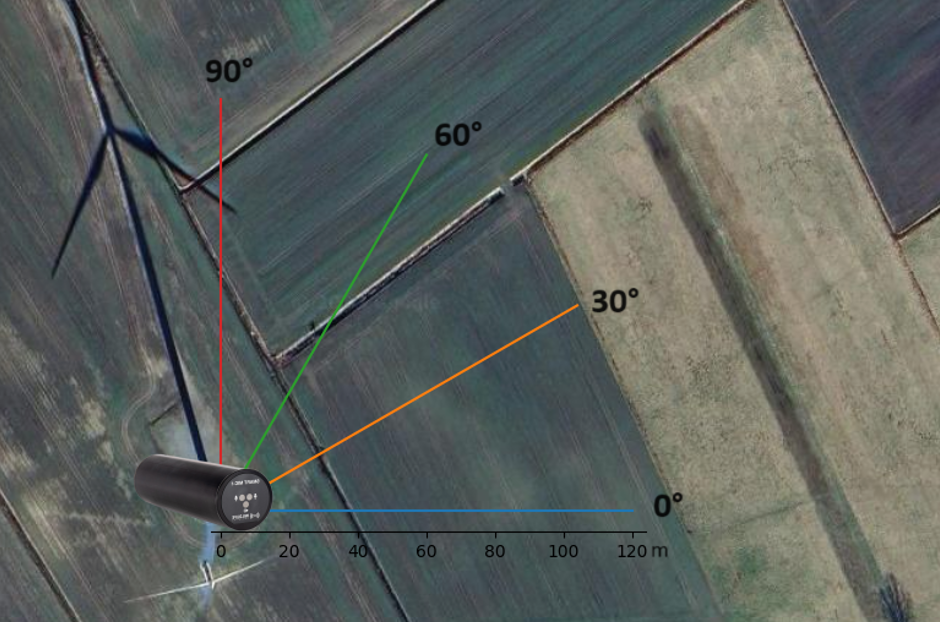
\includegraphics[width=0.8\textwidth]{sprz/angles.png}
  \caption{Zilustrowanie konfiguracji odległości i kątów od przodu mikrofonu, pod jakimi odtwarzane były dźwięki o poszczególnych częstotliwościach. Źródło: Google Maps}
  \label{img:angles}
\end{figure} 

\section{Realizacja testów w terenie}
Badania przeprowadzono w dniu 8 września 2023 roku zgodnie z przedstawioną powyżej metodyką w następujących warunkach atmosferycznych: 26 stopni C, zachmurzenie – 10\%, prędkość wiatru – 2-4 m/s, kierunek wiatru – NE, wilgotność – 40\% (\ref{img:fieldtests}).

\begin{figure}[h]
  \centering
  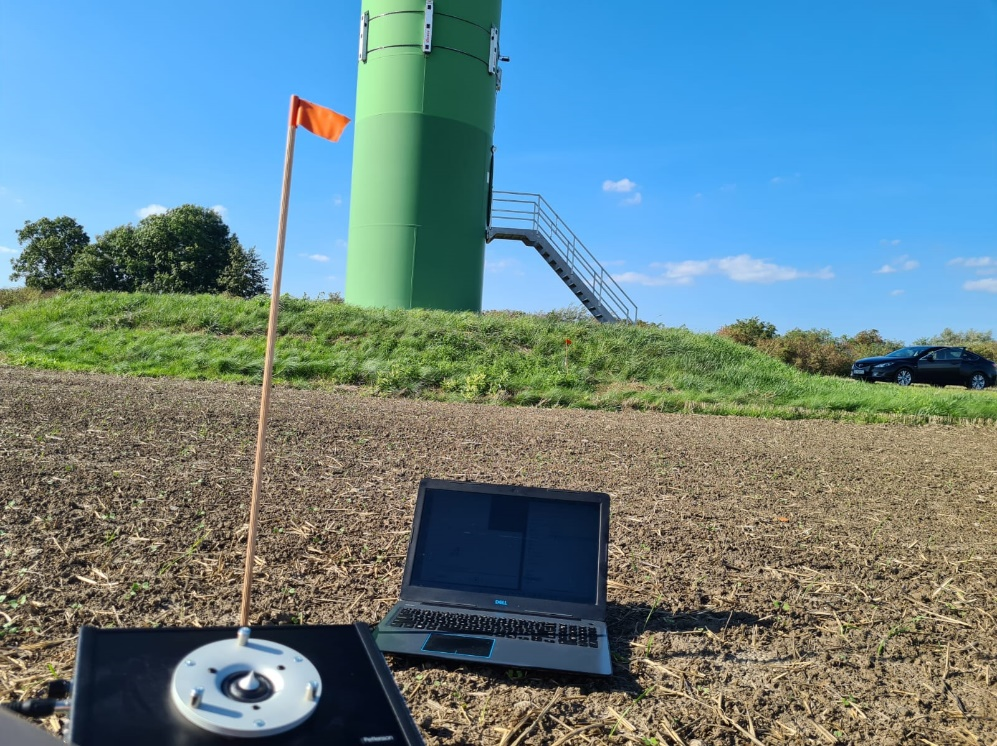
\includegraphics[width=0.8\textwidth]{sprz/fieldtests.png}
  \caption{Testy terenowe systemu SMART z użyciem głośnika Pettersson L400 i laptopa. Źródło: Bioseco}
  \label{img:fieldtests}
\end{figure}

\section{Wyniki testów}
Każda częstotliwość w każdej odległości i pod każdym kątem od mikrofonu została wyemitowana trzykrotnie (w większości przypadków). W wynikach uwzględniono jaki procent głosów w danej lokalizacji został wykryty, np. jeśli wykryto 2 odtworzenia na 4, to oznaczano wykrycie 50\% dźwięków.

Poniższe wykresy ilustrują odległości detekcji dźwięku w poszczególnych konfiguracjach odległości i kąta, w podziale na poszczególne częstotliwości (\ref{img:angle0}, \ref{img:angle30}, \ref{img:angle60}, \ref{img:angle90}).

  \begin{figure}[h]
    \centering
    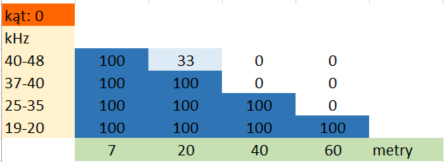
\includegraphics[width=0.8\textwidth]{sprz/angle0.png}
    \caption{Odległości detekcji dla poszczególnych częstotliwości pod kątem 0\textdegree do przodu mikrofonu.}
    \label{img:angle0}
  \end{figure}
\clearpage

  \begin{figure}[h]
    \centering
    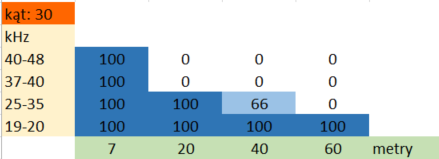
\includegraphics[width=0.8\textwidth]{sprz/angle30.png}
    \caption{Odległości detekcji dla poszczególnych częstotliwości pod kątem 30\textdegree do przodu mikrofonu.}
    \label{img:angle30}
  \end{figure} 

  \begin{figure}[h]
    \centering
    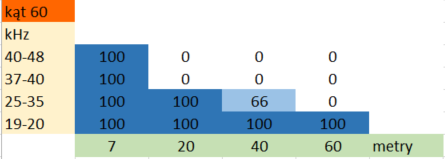
\includegraphics[width=0.8\textwidth]{sprz/angle60.png}
    \caption{Odległości detekcji dla poszczególnych częstotliwości pod kątem 60 do przodu mikrofonu.}
    \label{img:angle60}
  \end{figure} 

  \begin{figure}[h]
    \centering
    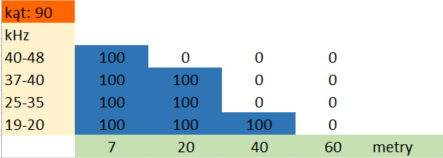
\includegraphics[width=0.8\textwidth]{sprz/angle90.png}
    \caption{Odległości detekcji dla poszczególnych częstotliwości pod kątem 90\textdegree do przodu mikrofonu.}
    \label{img:angle90}
  \end{figure}

\newpage
Na podstawie tych wyników można zauważyć następujące prawidłowości:
\begin{itemize}
  \item{Odległość detekcji ultradźwięków jest największa dla najniższych częstotliwości i maleje wraz ze wzrostem częstotliwości. Maksymalna odległość dotyczy częstotliwości 16-20 kHz i wynosi do 60 m, a najmniejsza odległość dla częstotliwości 37-48 kHz i wynosi do 20 m. Oznacza to, że gatunki takie jak borowiec i borowiaczek są wykrywane z odległości do 60 m, a karliki i inne nietoperze o wysokiej częstotliwości z maksymalnie 20 m.,}
  \item{Gdyby progi odległości były mniejsze, odległości wykrywania byłyby dokładniejsze i w większości przypadków wyższe,}
  \item{Częstotliwości 16-35 kHz są wykrywane równie dobrze, gdy dźwięki emitowane są pod kątem od 0\textdegree do 60\textdegree, wykrywalność zmniejsza się o 20-33\%, gdy dźwięki są emitowane pod kątem 90\textdegree,}
  \item{Dla wyższych częstotliwości – 37-48 kHz, większe znaczenie może mieć kąt padania dźwięku, gdyż w przypadku kątów 30\textdegree i 60\textdegree odległość detekcji zmniejsza się o ponad 50\% w porównaniu do kąta 0\textdegree. Niemniej jednak w przypadku częstotliwości 37-40 kHz przy 90\textdegree wykrywalność jest taka sama jak przy kącie 0\textdegree, dlatego wnioski nie są do końca jednoznaczne. Nie badano także odległości 10 i 15 m, co w tym przypadku mogłoby znacząco poprawić uzyskiwane pokrycie odległości.}
\end{itemize}

Maksymalne odległości detekcji nietoperzy odzywających się w poszczególnych zakresach częstotliwości odpowiadają odległościom obliczonym matematycznie dla tych częstotliwości \cite{agranat}, co pozwala ocenić, że system SMART wykrywa nietoperze z dużą skutecznością.

\section{Propozycja liczby i rozmieszczenia mikrofonów}
W celu przygotowania planu liczby i rozmieszczenia mikrofonów na turbinie wiatrowej wykorzystano informacje z konsultacji z firmą Wildife Acoustics oraz testów terenowych przeprowadzonych w ramach niniejszej pracy.

Z uwagi na dobre pokrycie kąta 180\textdegree przez jeden mikrofon, użycie dwóch mikrofonów na jednej wysokości pokryje kąt 360\textdegree.

Z uwagi na krótkie zasięgi wykrywania nietoperzy mikrofony powinny być zlokalizowane jak najbliżej łopat turbiny, tak by wykrywać aktywność w miejscu, w którym ich obecność może wiązać się z kolizjami, czyli w gondoli lub w dolnym zakresie łopaty. Z punktu widzenia ochrony nietoperzy optymalnym byłby montaż jednego lub dwóch mikrofonów w gondoli, i jednego lub dwóch w dolnym zasięgu łopaty na wieży. Ze względów praktycznych montaż oraz późniejszy dostęp do mikrofonów na poziomie dolnego zasięgu łopaty będzie drogi z uwagi na konieczny dostęp linowy oraz kłopotliwy z uwagi na brak opracowanego sposobu montażu w tym miejscu. Dlatego na obecnym etapie montaż powinien mieć miejsce w gondoli, bądź poprzez wywiercenie otworu w gondoli bądź montaż na szczycie gondoli na elementach takich jak barierki itp.
Mikrofon, bądź mikrofony wraz z kontrolerem powinny znajdować się razem w gondoli, gdyż długość kabla Ethernet jakiego można użyć do połączenia mikrofonu z kontrolerem wynosi 100 m, z uwagi na poprawność przesyłu danych. Gdy odległość od gondoli do podstawy wiatraka jest mniejsza niż 100 m, kontroler może znajdować się na dole wieży.

Odległości detekcji nietoperzy są na tyle małe w kontekście ich ochrony przed kolizjami z turbinami wiatrowymi, że klasyczne podejście oparte o system detekcyjno-reakcyjny polegające na wyłączeniu turbiny na podstawie każdego pojedynczego przelotu nie będzie przydatne, lecz konieczne będzie dobranie specyficznego wyzwalacza zatrzymującego i ponownie uruchamiającego turbinę, którym może być np. liczba zarejestrowanych przelotów nietoperzy w określonej jednostce czasu. W wyzwalaczach zatrzymań można użyć dodatkowo warunków środowiskowych, takich jak prędkość wiatru czy występowanie opadów (po połączeniu systemu SMART z systemem SCADA turbiny wiatrowej). Minimalizacje z zastosowaniem ograniczenia pracy turbin w określonych warunkach wiatrowych i opadów są obecnie stosowane w celu ograniczenia śmiertelności na farmach wiatrowych \cite{Wytyczne}

\chapter{Realizacja sieci neuronowej}

\section{Przygotowanie danych}
Przygotowanie danych obejmowało podpisanie nagrań zgodnie z wykazem gatunków nietoperzy przypisanych do danych nagrań, które znajdowały się w pliku CSV. Plik ten zawierał nazwę nagrania, datę jego zapisu oraz nazwę gatunkową nietoperza bądź informacje, że był to szum, bądź dźwięk niezidentyfikowany do gatunku. Finalnie w procesie przygotowania i uczenia sieci neuronowej nagrania zostały przetworzone do postaci tensorów, co zostało zrealizowane w module ładującym dane. Liczby wszystkich dźwięków wyniosła 18 412.

\subsection{Dobór typu spektogramu}
Do treningu użyto dźwięków przetworzonych na obrazy. Rozważano użycie zwykłego spektrogramu i mel-spektrogramu, jednak zdecydowano się na użycie zwykłego spektrogramu, ponieważ dawał on lepszy obraz. W przypadku bardzo delikatnych głosów nietoperzy na mel-spektrogramie pulsy były często niewidoczne.

\subsection{Cięcie}
W celu uzyskania jednolitych wielkości danych na wejściu wszystkie nagrania pocięto na odcinki dwusekundowe. W przypadku gdy ostatni element był krótszy niż dwie sekundy uzupełniano tę część zerami.

\section{Dobór sieci neuronowej}
Po przeglądzie literatury, konsultacjach z Aleksandrem Obuchowskim oraz weryfikacji zasobów czasowych zdecydowano się ostatecznie na użycie konwolucyjnej sieci neuronowej jako sieci przystępnej w implementacji a jednocześnie potencjalnie dającej bardzo dobre wyniki (por. "Przegląd literatury"). Sieci konwolucyjne były najczęściej używanymi sieciami neuronowymi. Inną architekturą mogącą dać bardzo dobre wyniki była sieć Transformers, na co wskazywały wyniki dostępnej publikacji oraz konsultacji z Aleksandrem Obuchowskim \cite{bats-transformers}. Z uwagi jednak na ograniczone dane literaturowe oraz ograniczone zasoby czasowe zaniechano realizacji tego typu architektury.

\subsection{Przegląd literatury}.
Do wyszukania publikacji zawierających opracowania dotyczące automatycznego rozpoznawania nietoperzy użyto wyszukiwarki Google Scholar oraz fraz: "bats automated recognition", "bats machine learning", "bats deep learning".

Do metod automatycznej identyfikacji gatunków nietoperzy wykorzystuje się
bądź wielowymiarowe metody statystyczne (jak np. analiza dyskryminacyjna czy wielowymiarowa analiza wariancji - MANOVA) \cite{bats-id-statistics}, bądź metody uczenia nadzorowanego \cite{bats-id-supervised} takie jak np.: sieci neuronowe \cite{bats-id-nn}, drzewa decyzyjne i lasy losowe \cite{bats-random-forest}, SVM (ang: Support Vector Machines) \cite{bats-id-svm}.

W przypadku sieci neuronowych, uczenia głębokiego do identyfikacji nietoperzy zaczęto używać dopiero w 2018 roku \cite{bats-id-dl2018}, a większą popularność sieci głębokie zdobyły od roku 2020 \cite{bats-id-dl2020a}, \cite{bats-id-dl2020b}, lecz publikacje takie są dość nieliczne.

Znaleziono tylko jedną pracę naukową, która wykorzystuje architekturę Transformers do rozpoznawania gatunków nietoperzy \cite{bats-transformers}.

Maksymalne skuteczności poszczególnych metod różnią się między sobą. Dla lasów losowych było to maksymalnie 83,1\% \cite{bats-id-randomforest} sieci neuronowych innych niż transformers było to maksymalnie 89,09\% precyzji \cite{bats-id-dl}, w przypadku modelu Transformers było to 90,2\% \cite{bats-transformers}.

\section{Dobór parametrów sieci neuronowej}

\subsection{Parametry warstw sieci}
Sieć konwolucyjna składa się z czterech bloków konwolucyjnych (z warstwą konwolucyjną, funkcją aktywacji ReLU i warstwą max-pooling), warstwy spłaszczającej do przestrzeni jednowymiarowej (warstwa "flatten"), warstwy fully-connected (w PyTorch nazywaną "linear") oraz ostatniej warstwy softmax, pozwalającej na uzyskanie wartości prawdopodobieństw przynależności nagrania do danej klasy (gatunku nietoperza).

Parametry pierwszej warstwy konwolucyjnej:
\begin{itemize}
  \item{liczba kanałów na wejściu - 1}
  \item{liczba kanałów na wyjściu (i liczba filtrów) - 16,}
  \item{rozmiar filtra ("kernel size") - 3,}
  \item {przesunięcie filtra ("stride") - 1,}
  \item{uzupełnienie skrajnych wartości ("padding") - 2.}
\end{itemize}

Parametry drugiej warstwy konwolucyjnej:
Warstwa konwolucyjna
\begin{itemize}
  \item{liczba kanałów na wejściu - 16}
  \item{liczba kanałów na wyjściu (i liczba filtrów) - 32,}
  \item{rozmiar filtra ("kernel size") - 3,}
  \item {przesunięcie filtra ("stride") - 1,}
  \item{uzupełnienie skrajnych wartości ("padding") - 2.}
\end{itemize}

Parametry trzeciej warstwy konwolucyjnej:
\begin{itemize}
  \item{liczba kanałów na wejściu - 32}
  \item{liczba kanałów na wyjściu (i liczba filtrów) - 64,}
  \item{rozmiar filtra ("kernel size") - 3,}
  \item {przesunięcie filtra ("stride") - 1,}
  \item{uzupełnienie skrajnych wartości ("padding") - 2.}
\end{itemize}

Parametry czwartej warstwy konwolucyjnej:
\begin{itemize}
  \item{liczba kanałów na wejściu - 64}
  \item{liczba kanałów na wyjściu (i liczba filtrów) - 128,}
  \item{rozmiar filtra ("kernel size") - 3,}
  \item {przesunięcie filtra ("stride") - 1,}
  \item{uzupełnienie skrajnych wartości ("padding") - 2.}
\end{itemize}

W każdej z warstw konwolucyjnych zastosowano funkcję aktywacji ReLU i warstwę max-pooling o filtrze w rozmiarze 2 ("stride").

\subsection{Funkcje aktywacji}
Funkcja aktywacji używana jest do obliczania wartości neuronów w warstwach wyjściowych.

W warstwach konwolucyjnych jako funkcji aktywacji użyto funkcji ReLU (Rectified Linear Unit). Jest to najczęściej używana funkcja aktywacji w warstwach ukrytych. Do jej zalet należą szybkość i nieliniowość.

W ostatniej warstwie użyto funkcji aktywacji softmax. Przekształca ona wartości uzyskiwane na wyjściu tak, aby ich suma była równa 1, dzięki czemu dobrze modeluje prawdopodobieństwo. Jest to najczęściej wykorzystywana funkcja w warstwach wyjściowych.

\subsection{Funkcja błędu}
Funkcja ta jest często używana w sieciach neuronowych w problemach klasyfikacji. Określa ona jak dobrze model przewiduje klasy - im mniejsza wartość funkcji błędu, tym większa dokładność modelu. Podczas uczenia się sieci dąży się do zmniejszania wartości funkcji błędu. W sieci neuronowej użytej w niniejszej pracy wykorzystano funkcję entropii krzyżowej.

\subsection{Optymalizator}
Optymalizator jest to funkcja lub algorytm decydująca o tym jak zmienić wagi sieci na podstawie funkcji błędu, tak aby zmniejszyć wartość tej funkcji. Optymalizator wpływa na to jak szybko sieć będzie się uczyć poprzez zmianę jej parametrów oraz jak poradzi sobie z problemami takimi jak utknięcie w lokalnym minimum. W sieci neuronowej przedstawionej w niniejszej pracy wykorzystano optymalizator Adam (Adaptive Moment Estimation). Optymalizator ten jest najczęściej wykorzystywanym i dającym najczęściej najlepsze wyniki.

\section{Architektura sieci neuronowej i modułów związanych z treningiem sieci}
Sieć neuronowa napisana została w języku Python, z użyciem biblbiotek PyTorch oraz TorchAudio. 

PyTorch jest biblioteką oferującą narzędzia do budowy i trenowania sieci neuronowych, zawiera m.in. moduły do tworzenia warstw sieci, funkcji straty czy optymalizatorów, daje wsparcie do trenowania na kartach graficznych \cite{pytorch}.
PyTorch jest biblioteką o podobnej popularności co Tensorflow, a w ostatnich latach nawet częściej wykorzystywaną, szczególnie w środowiskach akademickich. Umożliwia ona na większą elastyczność w budowie sieci i ustawieniach jej parametrów. Do zalet takiego rozwiązania należy większy wpływ na kształt i funkcjonowanie sieci, a do wad - dłuższy czas przygotowania oraz wyższy próg wejścia. 

Biblioteka TorchAudio jest częścią ekosystemu PyTorch i służy do obsługi i obróbki plików dźwiękowych. Dostarcza narzędzi pomocnych w ładowaniu danych audio oraz transformacjach takich jak zmiany prędkości czy głośności, przetwarzanie na spektrogramy czy mel-spektrogramy \cite{torchaudio}. 

Sień neuronowa przygotowana w ramach niniejszej pracy dyplomowej składa się z czterech głównych elementów: modułu transformującego dźwięk do spektrogramów, modułu ładującego dane, modułu do treningu oraz modułu do predykcji.

\subsection{Konwersja dźwięków na spektrogramy}
Identyfikacja gatunków nietoperzy poprzez analizę dźwięków skonwertowanych do obrazu jest podejściem klasycznym (por. np. \cite{bats-id-dl2020b}). Dlatego jednym z elementów związanych z trenowaniem sieci było przygotowanie modułu konwertującego dźwięk na spektrogramy. Kod modułu przedstawiono poniżej w Listingu \ref{lst:audio-to-spektrogram}. Ścieżki bezwzględne zostały użyte dlatego, że kod ten służył jedynie do treningu i uczenia sieci.

\begin{lstlisting}[language=Python,caption={Implementacja konwersji dźwięku na spektrogram}, label={lst:audio-to-spektrogram}]
  waveform, sample_rate = torchaudio.load(r'C:\\Users\\Jakub\Documents\\PJATK\\INZ\Batmonit_model\\Chiro_sounds_signed\Audio\\PIPNAT\S4U08639_20210731_234142_PIPNAT.wav')
  fragments = torch.split(waveform, split_size_or_sections=2*sample_rate, dim=1)
  
  specgram = torchaudio.transforms.Spectrogram(
          )(fragments[1])
  
  plt.figure(figsize=(12, 8))
  plt.imshow(specgram[0].log2(), aspect='auto', origin='lower')
  plt.show()
\end{lstlisting}

\subsection{Ładowanie danych}

Moduł ładujący dane jest najbardziej rozbudowanym elementem architektury związanej z treningiem sieci. Składa się z wielu funkcji, które zapewniają identyczność parametrów każdego z nagrań, takich jak liczba kanałów czy wielkość obrazu. Zawiera również funkcji odpowiedzialne za pobieranie ścieżek plików.

Poniżej w Listingu \ref{lst:audio-to-spectrogram} przedstawiono jedną z takich funkcji. Służy ona do konwersji częstotliwości próbkowania, jeśli byłaby ona inna niż założona pierwotnie dla wszystkich nagrań.

\begin{lstlisting}[language=Python,caption={Implementacja konwersji dźwięku na spektrogram}, label={lst:audio-to-spectrogram}]
  def _resample_if_necessery(self, signal, sr):
  if sr != self.target_sample_rate:
      resampler = torchaudio.transforms.Resample(sr, self.target_sample_rate)
      signal = resampler(signal)
  return signal
\end{lstlisting}

Główna funkcja tego modułu uruchamia ładowanie danych z uwzględnieniem wszystkich wyżej wymienionych elementów i przedstawiono ją poniżej w Listingu \ref{lst:audio-to-spectrogram}.

\begin{lstlisting}[language=Python,caption={Implementacja modułu do ładowania danych}, label={lst:audio-to-spectrogram}]
  if __name__ == "__main__":
  ANNOTATIONS_FILE = r"C:\Users\Jakub\Documents\PJATK\INZ\Batmonit_model\Chiro_sounds_signed\Metadata\Annotations.csv"
  AUDIO_DIR = r"C:\Users\Jakub\Documents\PJATK\INZ\Batmonit_model\Chiro_sounds_signed\Audio"
  SPECTROGRAM_DIR = r"C:\Users\Jakub\Documents\PJATK\INZ\Batmonit_model\Chiro_sounds_signed\Spectrogram"
  SAMPLE_RATE = 192000
  NUM_SAMPLES = 2000000

  if torch.cuda.is_available():
      device = "cuda"
  else:
      device = "cpu"
  print(f"Using device: {device}")

  spectrogram = torchaudio.transforms.Spectrogram(
      n_fft=1024,
      hop_length=1024,
  )
  bd = BatsDataset(ANNOTATIONS_FILE,
                          AUDIO_DIR,
                          SPECTROGRAM_DIR, 
                          spectrogram, 
                          SAMPLE_RATE,
                          NUM_SAMPLES,
                          device)

  print(f"There are {len(bd)} samples in the dataset.")
  signal, label = bd[0]
  print(signal, label)
\end{lstlisting}

\subsection{Sień neuronowa}
Kod sieci neuronowej przedstawiono poniżej w Listingu \ref{lst:Sequelize_validate}, a wyjaśnienie zastosowania konkretnych jej elementów, takich jak funkcje aktywacji, funkcja błędu, optymalizator, itd. opisano i wyjaśniono w rozdziale: "Dobór parametrów sieci neuronowej". Implementację sieci neuronowej przedstawia Listing \ref{lst:neural_network_implementation}.
Architektura sieci została zaprojektowana z uwzględnieniem następujących informacji:
\begin{itemize}
  \item{potencjalnych możliwości sprzętu używanego do treningu,}
  \item{informacji o konstrukcji sieci neuronowych dostępnych w literaturze,}
  \item{informacji o konstrukcji sieci neuronowych wykorzystywanych do identyfikacji nietoperzy.}
\end{itemize}

Architekturę sieci wybrano na podstawie dostępnej literatury, która obfituje w dane o wykorzystaniu sieci konwolucyjnych dających dobre wyniki w identyfikacji nietoperzy. Konstrukcja zastosowanej sieci konwolucyjnej należy z kolei do klasycznych, gdzie po warstwach konwolucyjnych i max-pool, znajdują się warstwy spłaszczające, fully-connected oraz softmax \cite{obuchowski}
Przyjęto możliwie małą liczbę warstw konwolucyjnych, aby w przypadku konieczności trenowania na własnych urządzeniach proces ten był wykonalny dla sprzętu w okresie, nie uniemożliwiającym realizację pracy dyplomowej. Jednocześnie liczba warstw konwolucyjnych miała znajdować się w przedziale tych używanych w innych projektach por. np. \cite{bats-id-randomforest}. 

\begin{lstlisting}[language=Python,caption={Implementacja sieci neuronowej}, label={lst:neural_network_implementation}]
  class CNNNetwork(nn.Module):

  def __init__(self):
      super().__init__()
      self.conv1 = nn.Sequential(
          nn.Conv2d(
              in_channels=1, 
              out_channels=16,  
              kernel_size=3,  
              stride=1,
              padding=2
          ),
          nn.ReLU(),
          nn.MaxPool2d(kernel_size=2)  
      )
      self.conv2 = nn.Sequential(
          nn.Conv2d(
              in_channels=16,
              out_channels=32,
              kernel_size=3,
              stride=1,
              padding=2
          ),
          nn.ReLU(),
          nn.MaxPool2d(kernel_size=2)
      )
      self.conv3 = nn.Sequential(
          nn.Conv2d(
              in_channels=32,
              out_channels=64,
              kernel_size=3,
              stride=1,
              padding=2
          ),
          nn.ReLU(),
          nn.MaxPool2d(kernel_size=2)
      )
      self.conv4 = nn.Sequential(
          nn.Conv2d(
              in_channels=64,
              out_channels=128,
              kernel_size=3,
              stride=1,
              padding=2
          ),
          nn.ReLU(),
          nn.MaxPool2d(kernel_size=2)
      )
      self.flatten = nn.Flatten()
      self.linear = nn.Linear(128*33*13, 14) 
                                             
      self.softmax = nn.Softmax(dim=1)

  def forward(self, input_data):
      x = self.conv1(input_data)
      x = self.conv2(x)
      x = self.conv3(x)
      x = self.conv4(x)
      x = self.flatten(x)
      logits = self.linear(x)
      predictions = self.softmax(logits)
      return predictions

if __name__ == "__main__":
  cnn = CNNNetwork()
\end{lstlisting}

\subsection{Trenowanie modelu}
Moduł związany z trenowaniem sieci neuronowej składał się z funkcji służącej do stworzenia dataloader'a, trenowania pojedynczej epoki oraz treningu kolejnych epok. Wielkość batch'a określono na 128, liczbę epok na 10, a wskaźnik uczenia na 0,001.

Główną funkcję przedstawiono w Listingu \ref{lst:train} poniżej.

\begin{lstlisting}[language=Python,caption={Implementacja modułu do trenowania sieci}, label={lst:train}]
  if __name__ == "__main__":

  if torch.cuda.is_available():
      device = "cuda"
  else:
      device = "cpu"
  print(f"Using device: {device}")

  spectrogram = torchaudio.transforms.Spectrogram(
      n_fft=1024,
      hop_length=1024,
  )

  bd = BatsDataset(ANNOTATIONS_FILE,
                          AUDIO_DIR,
                          SPECTROGRAM_DIR, 
                          spectrogram, 
                          SAMPLE_RATE,
                          NUM_SAMPLES,
                          device)


  train_data_loader = create_data_loader(bd, batch_size=BATCH_SIZE)

  cnn = CNNNetwork().to(device)

  loss_fn = nn.CrossEntropyLoss()
  optimiser = torch.optim.Adam(cnn.parameters(), lr=LEARNING_RATE)

  train(cnn, train_data_loader, loss_fn, optimiser, device, EPOCHS)

  torch.save(cnn.state_dict(), MODEL_PATH)

  print("Model trained and stored at feedforwardnet.pth")
\end{lstlisting}

\subsection{Predykcja modelu}
Moduł służący do wykonania predykcji zawiera poza główną funkcją dwa elementy - mapowanie klas (gatunków nietoperzy) oraz funkcję służącą do realizacji predykcji, która z użyciem wytrenowanego wcześniej modelu przewiduje gatunki nietoperzy na zbiorze testowym.

Kod głównej funkcji przedstawiono w Listingu \ref{lst:predict} poniżej.

\begin{lstlisting}[language=Python,caption={Implementacja modułu do trenowania sieci}, label={lst:predict}]
  if __name__ == "__main__":

  cnn = CNNNetwork()
  state_dict = torch.load(r"C:\Users\Jakub\Documents\PJATK\INZ\Batmonit_model\feedforwardnet.pth", map_location=torch.device('cpu'))
  cnn.load_state_dict(state_dict)

  spectrogram = torchaudio.transforms.Spectrogram(
      n_fft=1024,
      hop_length=1024,
  )

  bd = BatsDataset(ANNOTATIONS_FILE,
                          AUDIO_DIR,
                          SPECTROGRAM_DIR, 
                          spectrogram, 
                          SAMPLE_RATE,
                          NUM_SAMPLES,
                          "cpu")

  input, target = bd[0][0], bd[0][1]
  input.unsqueeze_(0)

  predicted, expected = predict(cnn, input, target,
   class_mapping)

  print(f"Predicted: '{predicted}', expected: '{expected}'")
\end{lstlisting}

\section{Skuteczność sieci neuronowej}
Dokładność sieci neuronowej wyniosła poniżej 75\% w związku z czym, nie udało się zrealizować założonego poziomu dokładności.

\chapter{Struktura systemu}

Struktura wytworzonego systemu została przedstawiona w podziale na poszczególne komponenty.

\section{Schemat połączeń}
System SMART na turbinie wiatrowej połączony jest do sieci internetowej, gdzie skonfigurowane jest połączenie do sieci Bioseco S.A.. Komputer firmowy, na którym skonfigurowane jest połączenie do sieci Bioseco S.A. przez VPN łączy się zdalnie z systemem SMART, dzięki czemu możliwy jest dostęp do danych z mikrofonu (\ref{img:system-connection}).

\begin{figure}[h] 
  \centering
  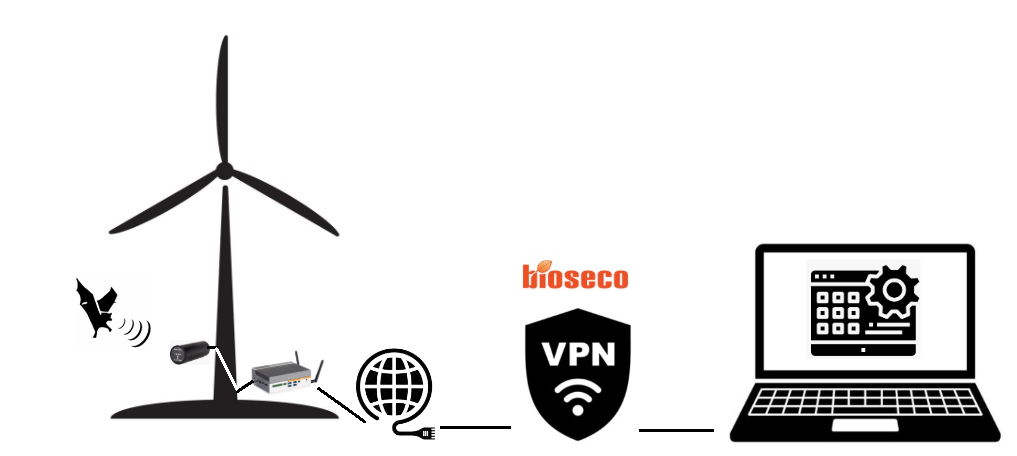
\includegraphics[width=0.8\textwidth]{sprz/system-connection.png}
  \caption{Schemat połączeń sieciowych pomiędzy systemem SMART i komputerem, na którym uruchomiona jest aplikacja.}
  \label{img:system-connection}
\end{figure} 

\section{Architektura systemu}

Na poniższych modelach przedstawiono najważniejsze elementy logiczne, urządzenia wejścia-wyjścia oraz obieg informacji w systemie (\ref{img:architektura_systemu2}). W celu ułatwienia zrozumienia osadzenia systemu w rzeczywistości, architekturę zobrazowano również w postaci graficznej, łącznie z widokiem interfejsu (\ref{img:reprezentacja_graficzna}). 

Spośród przedstawionych elementów cały moduł detekcji był zrealizowany poprzez dostarczony przez Bioseco S.A. system SMART firmy Wildlife Acoustics. Składa się on z mikrofonu ultradźwięków i kontrolera. Dźwięki z mikrofonu są rejestrowane przez program firmy Wildlife Acoustics na kontrolerze. Połączenie LAN zostało zrealizowane przez pracowników firmy Bioseco S.A.

Moduł decyzyjny stanowiło wytworzone oprogramowanie składające się z Watchdoga, będącego mikroserwisem monitorującym pojawienie się nowych nagrań i identyfikującym nietoperze, bazy danych do której te informacje trafiały oraz interfejsu użytkownika, który je wizualizował.

Szczegóły procesu przepływu danych od mikrofonu do interfejsu użytkownika zaprezentowano w rozdziale "System w działaniu".

\begin{figure}[h]
    \centering
    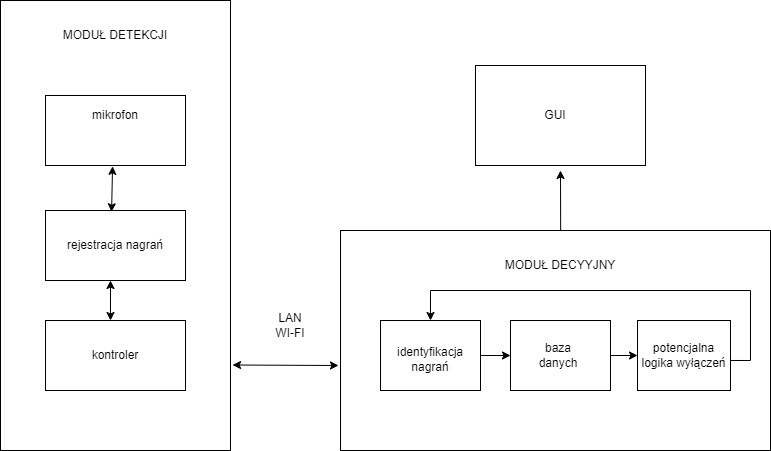
\includegraphics[width=1.0\textwidth]{sprz/architektura_systemu2.png}
    \caption{Logiczny model architektury systemu}
    \label{img:architektura_systemu2}
\end{figure}
\clearpage

\begin{figure}[h]
    \centering
    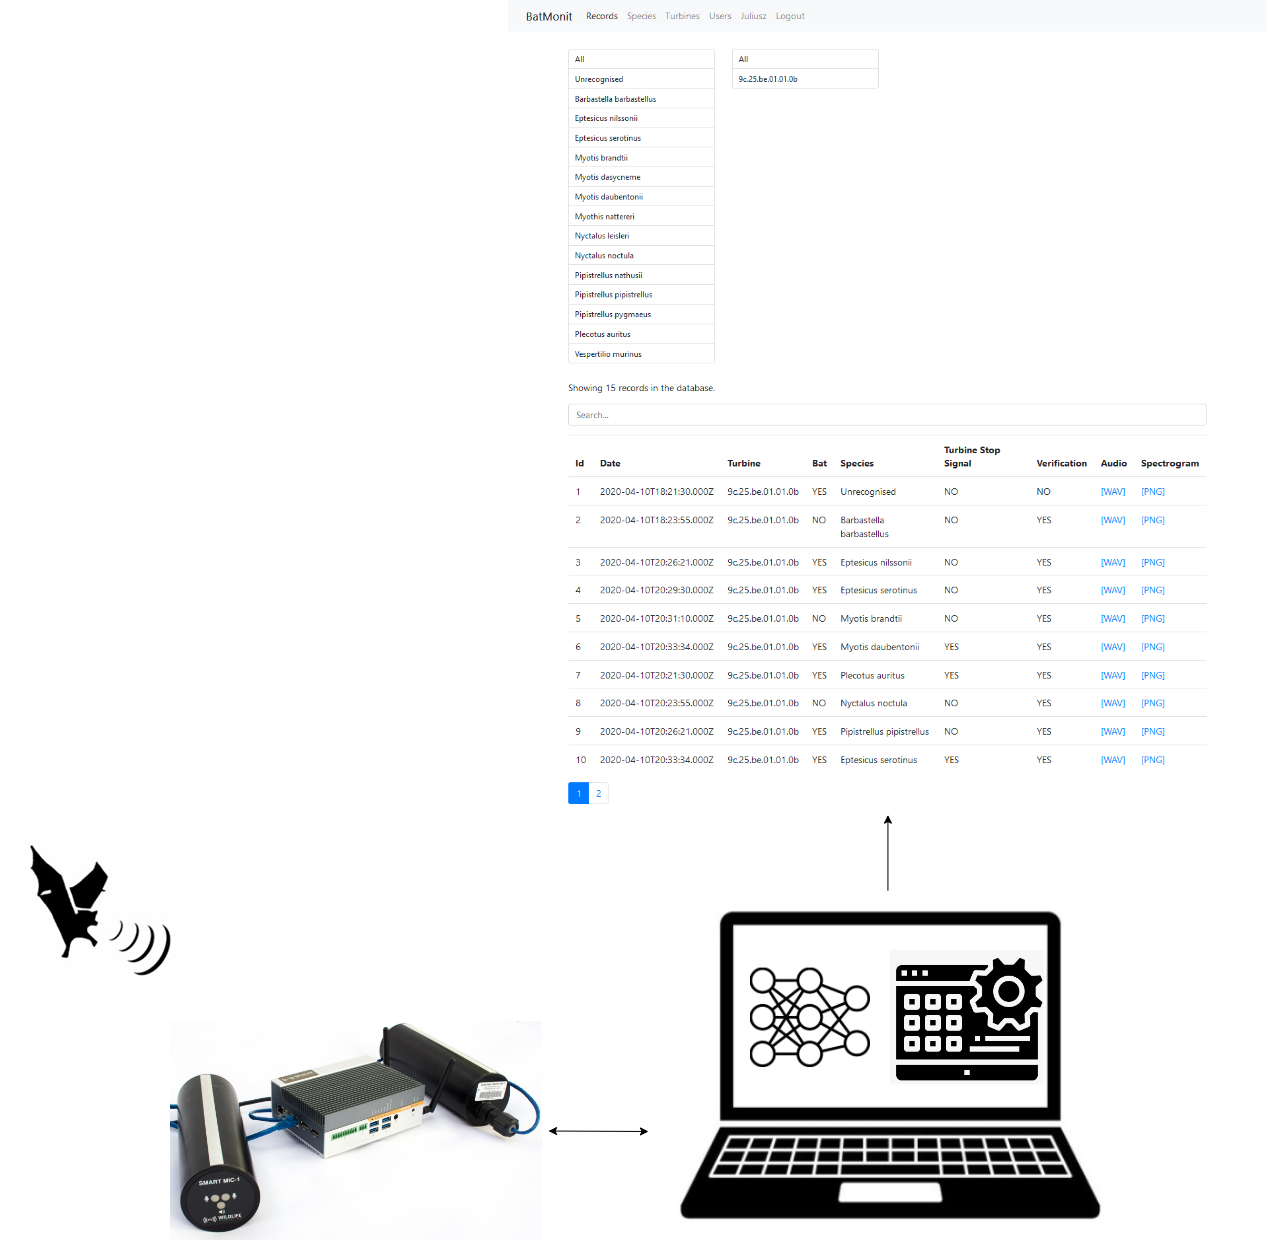
\includegraphics[width=1.0\textwidth]{sprz/graficzna-reprezentacja-systemu.png}
    \caption{Graficzna reprezentacja architektury systemu}
    \label{img:reprezentacja_graficzna}
\end{figure}

\section{Hardware}
Kluczowe zasoby sprzętowe rozwiązania, to system SMART firmy Wildlife Acoustics. Składa się on z mikrofonu ultradźwięków oraz tzw. kontrolera, będącego prostym przemysłowym komputerem. Mikrofon jest połączony z kontrolerem kablem Ethernet, co pozwala na zasilanie mikrofonu oraz przesył danych pomiędzy tymi komponentami. Dane z mikrofonu pobierane są przez oprogramowanie Wildlife Acoustics zainstalowane na kontrolerze i tam też są one gromadzone.
\clearpage

\begin{figure}[h]
  \centering
  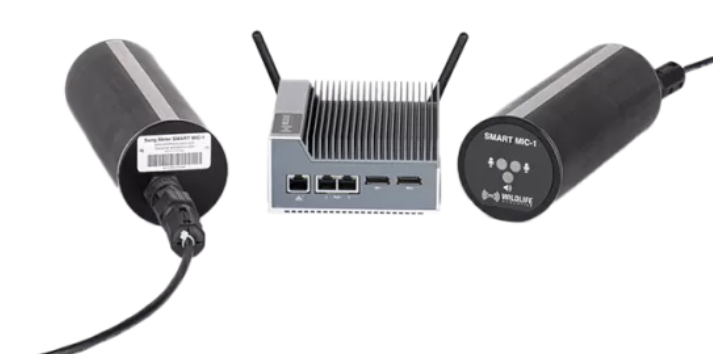
\includegraphics[width=0.8\textwidth]{sprz/smart2}
  \caption{system SMART - mikrofon ultradźwięków i kontroler}
  \label{img:smart2}
\end{figure}

\section{Model sieci neuronowej}
Jednym z elementów oprogramowania był model sieci neuronowej. 

Do treningu i predykcji gatunków nietoperzy użyta został sieć konwolucyjna składająca się z czterech bloków konwolucyjnych (z warstwą konwolucyjną, funkcją aktywacji ReLU i warstwą max-pooling), warstwy spłaszczającej do przestrzeni jednowymiarowej (warstwa flatten), warstwy fully-connected (w PyTorch nazywaną "linear") oraz ostatniej warstwy softmax, pozwalającej na uzyskanie wartości prawdopodobieństw przynależności nagrania do danej klasy (gatunku nietoperza).

W każdej z warstw konwolucyjnych zastosowano funkcję aktywacji ReLU i warstwę max-pooling o filtrze w rozmiarze 2 ("stride").

Szczegóły związane z uzasadnieniem implementacji danej architektury sieci zostały opisane w rozdziale "Realizacja sieci neuronowej".
\clearpage

\section{Aplikacja użytkownika}

Aplikacja użytkownika służy użytkownikowi do przeglądania rekordów tworzonych przez model na podstawie zarejestrowanych nagrań. Do celu nawigacji po aplikacji służy pasek menu w górnej części ekranu, który zawiera odnośniki do poszczególnych widoków.

Widok rejestracji (\ref{img:app_register}) pozwala na zarejestrowanie nowego użytkownika. Po dokonaniu rejestracji nowy użytkownik automatycznie zostaje zalogowany. Po zalogowaniu w pasku menu pojawia się przycisk \textit{Logout} służący do wylogowania aktualnie zalogowanego użytkownika.
\begin{figure}[h]
  \centering
  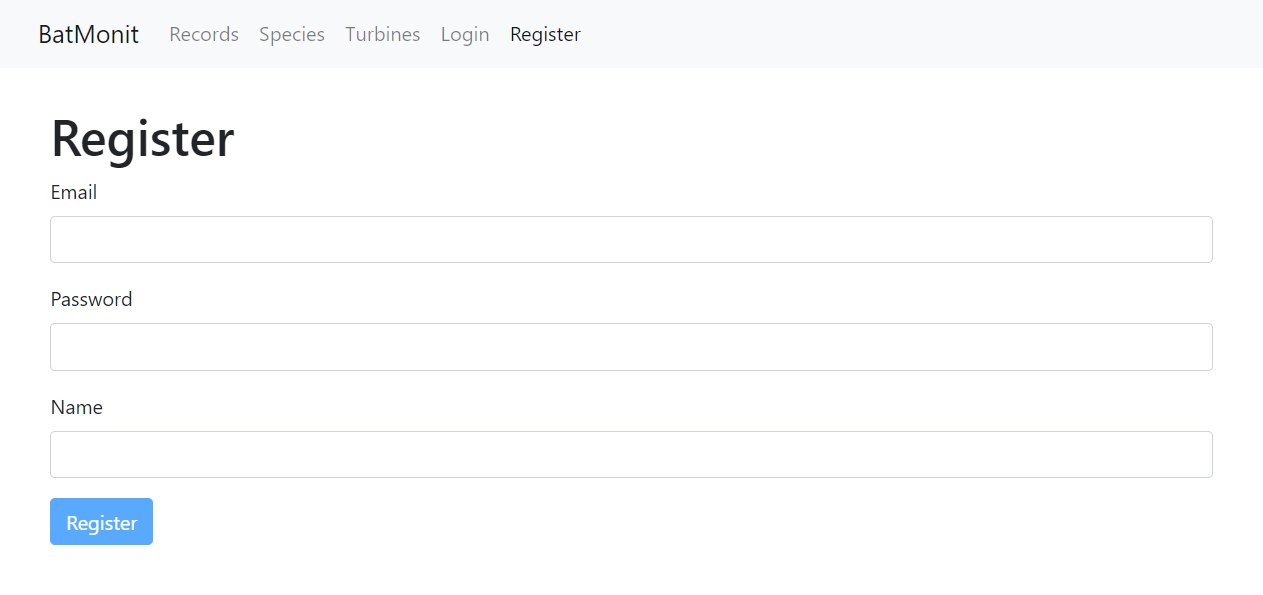
\includegraphics[width=0.8\textwidth]{sprz/app_register}
  \caption{Widok rejestracji użytkownika}
  \label{img:app_register}
\end{figure}

Diagram sekwencji przedstawiony na Rysunku \ref{img:sequence_register} obrazuje logikę działania modułu rejestracji. Po wprowadzeniu przez użytkownika danych i potwierdzeniu przyciskiem Register, aplikacja sprawdza, czy takich użytkownik już istnieje w systemie. Jeśli tak, to zwracana jest odpowiedź, że taki użytkownik nie może zostać ponownie zarejestrowany. Jeśli nie istnieje, to użytkownik zostaje zarejestrowany.

\begin{figure}[h]
  \centering
  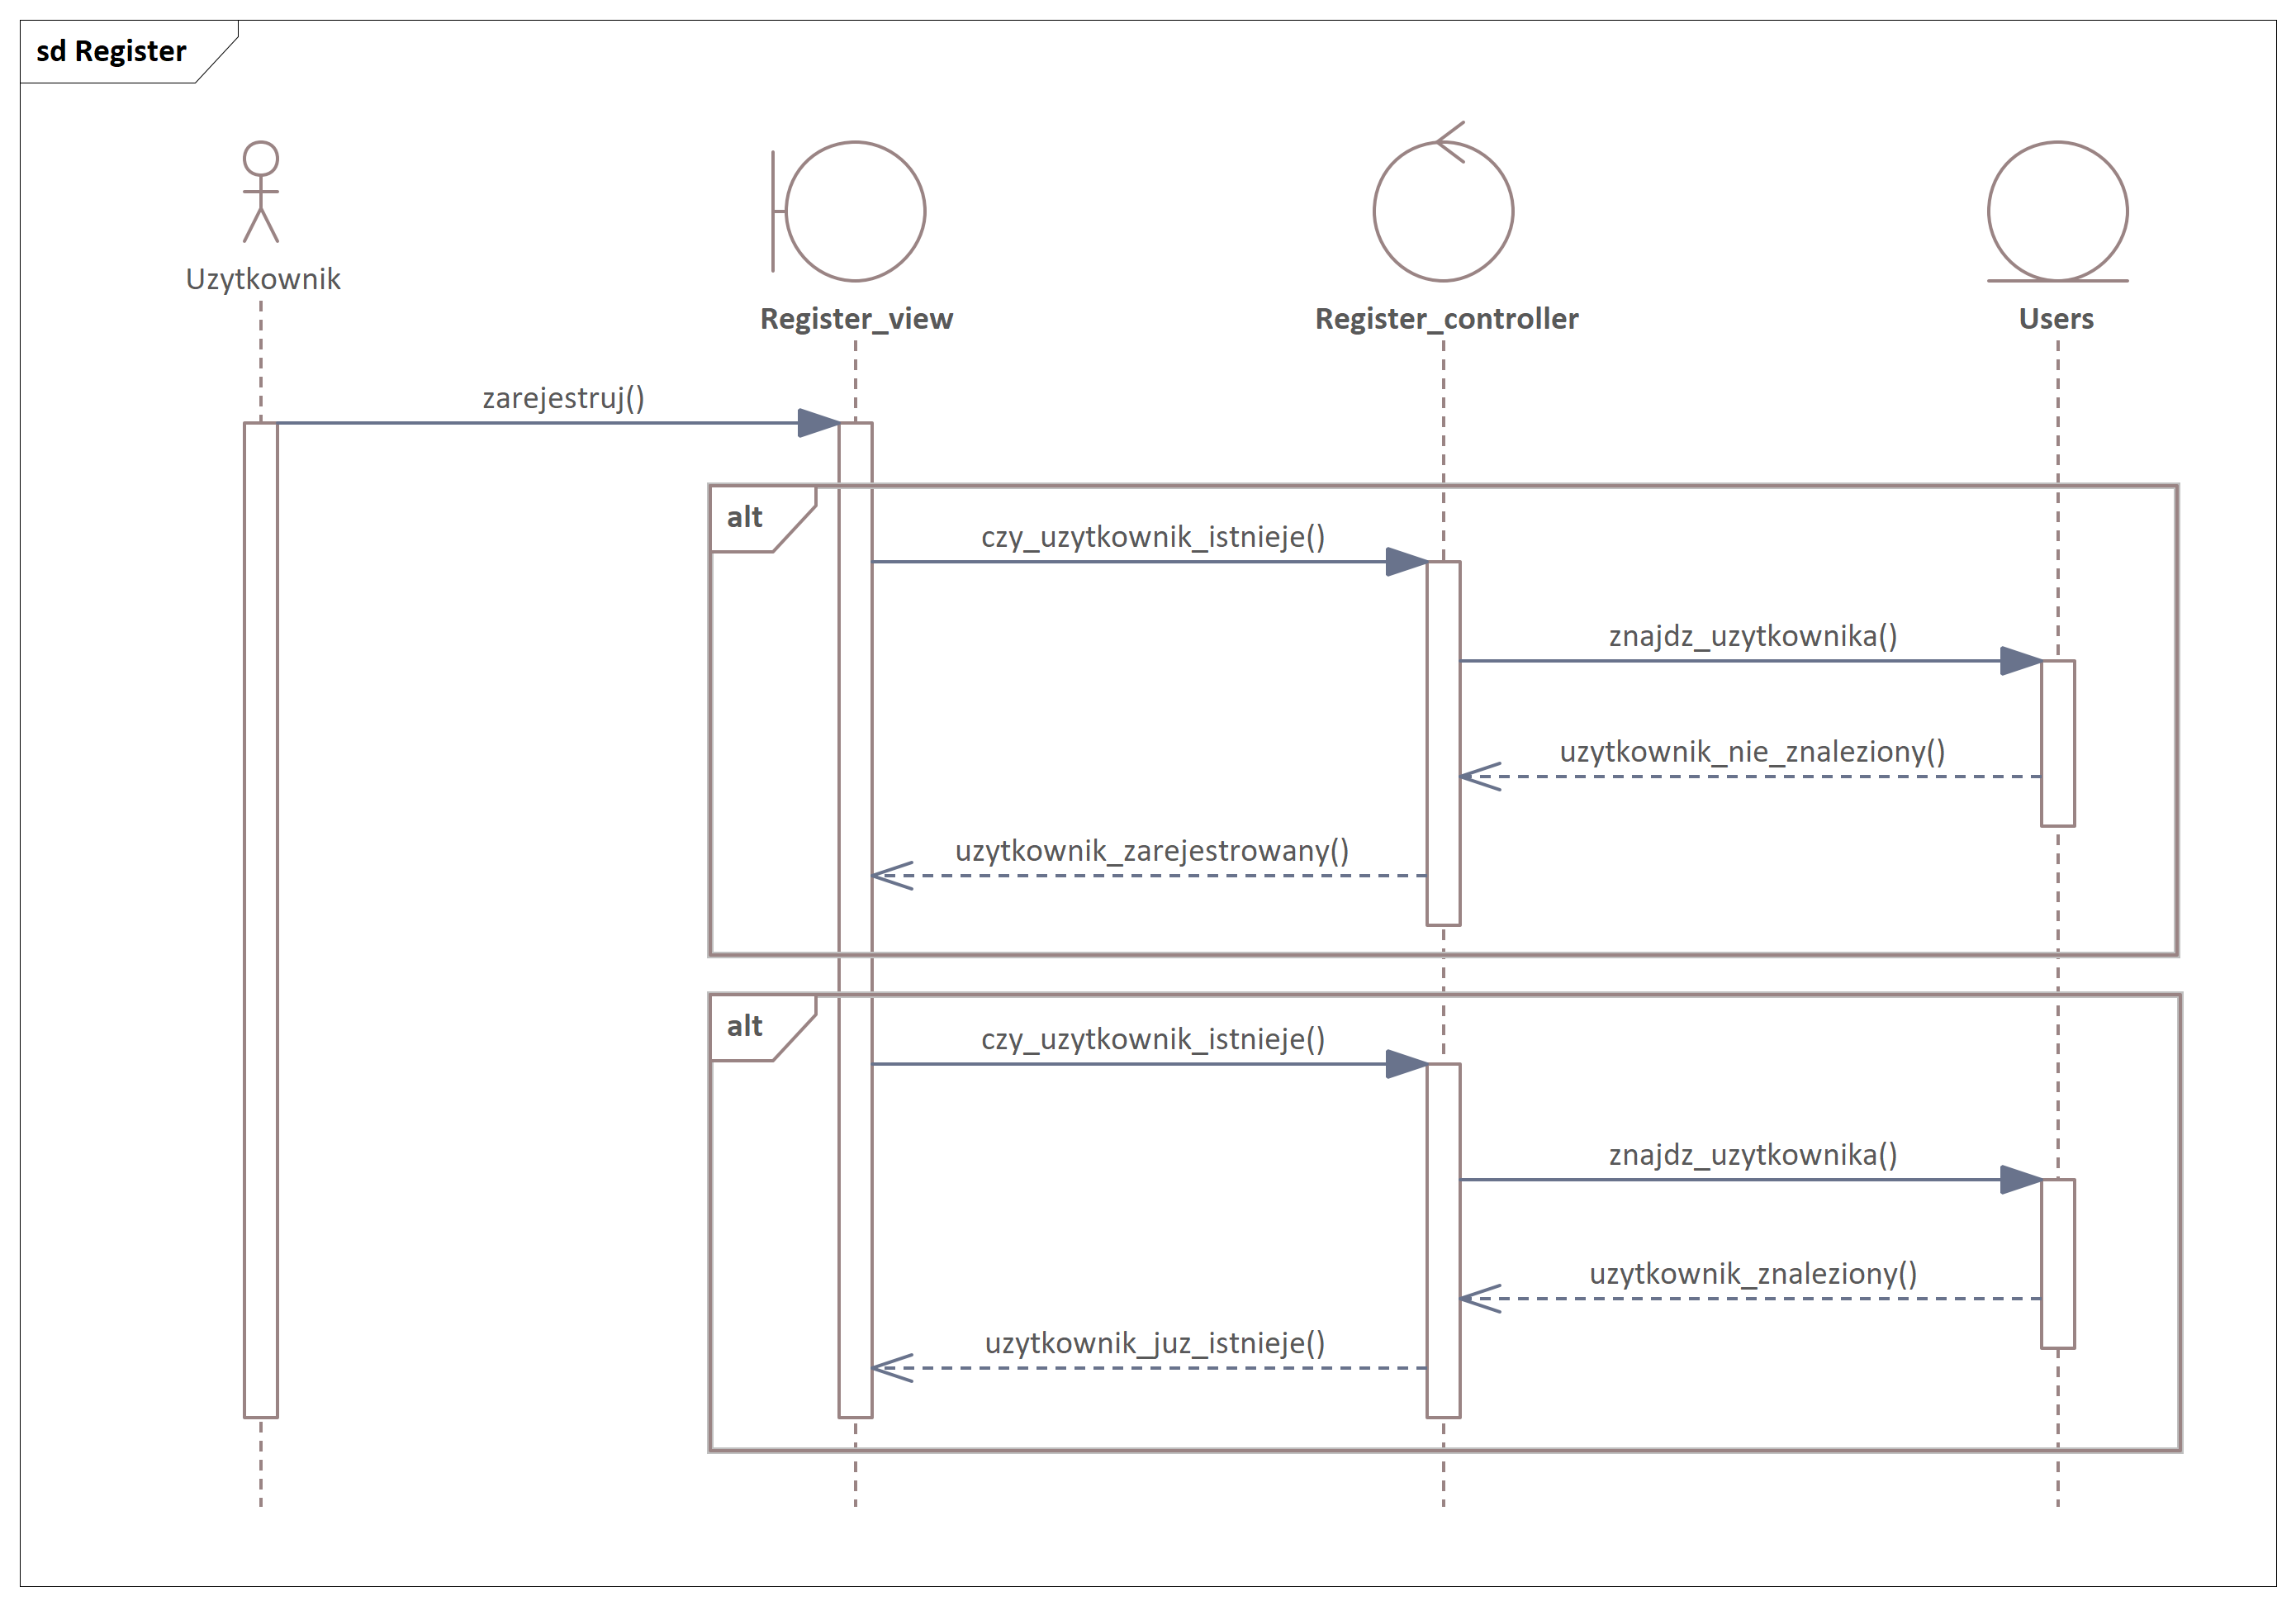
\includegraphics[width=0.9\textwidth]{sprz/sequence_register}
  \caption{Diagram sekwencji dla rejestracji}
  \label{img:sequence_register}
\end{figure}

Do celu zalogowania istniejącego już użytkownika służy widok logowania (\ref{img:app_login}).
\begin{figure}[h]
  \centering
  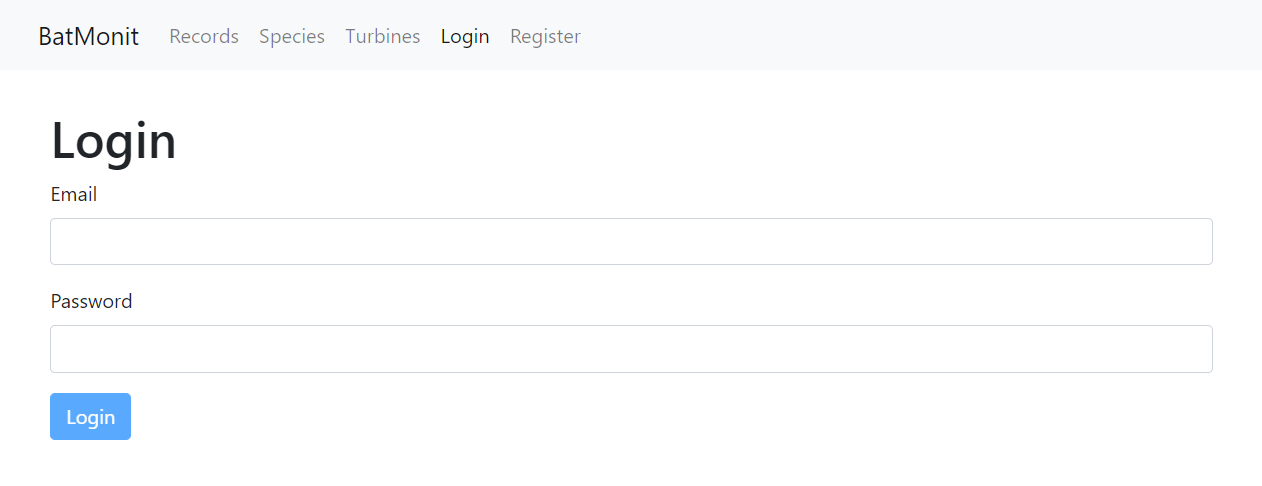
\includegraphics[width=0.8\textwidth]{sprz/app_login}
  \caption{Widok logowania użytkownika}
  \label{img:app_login}
\end{figure}

Diagram sekwencji z Rysunku \ref{img:sequence_login} przedstawia logikę logowania. Po wpisaniu przez użytkownika danych logowania i potwierdzenia przyciskiem Login, aplikacja sprawdza, czy taki użytkownik istnieje. Jeśli tak, to sprawdza, czy wprowadzone hasło jest poprawne. Jeśli tak, to użytkownik zostaje zalogowany. W wypadku gdy użytkownik nie istnieje lub podane hasło jest niepoprawne, aplikacja zwraca komunikat o nieprawidłowych danych logowania.

\begin{figure}[h]
  \centering
  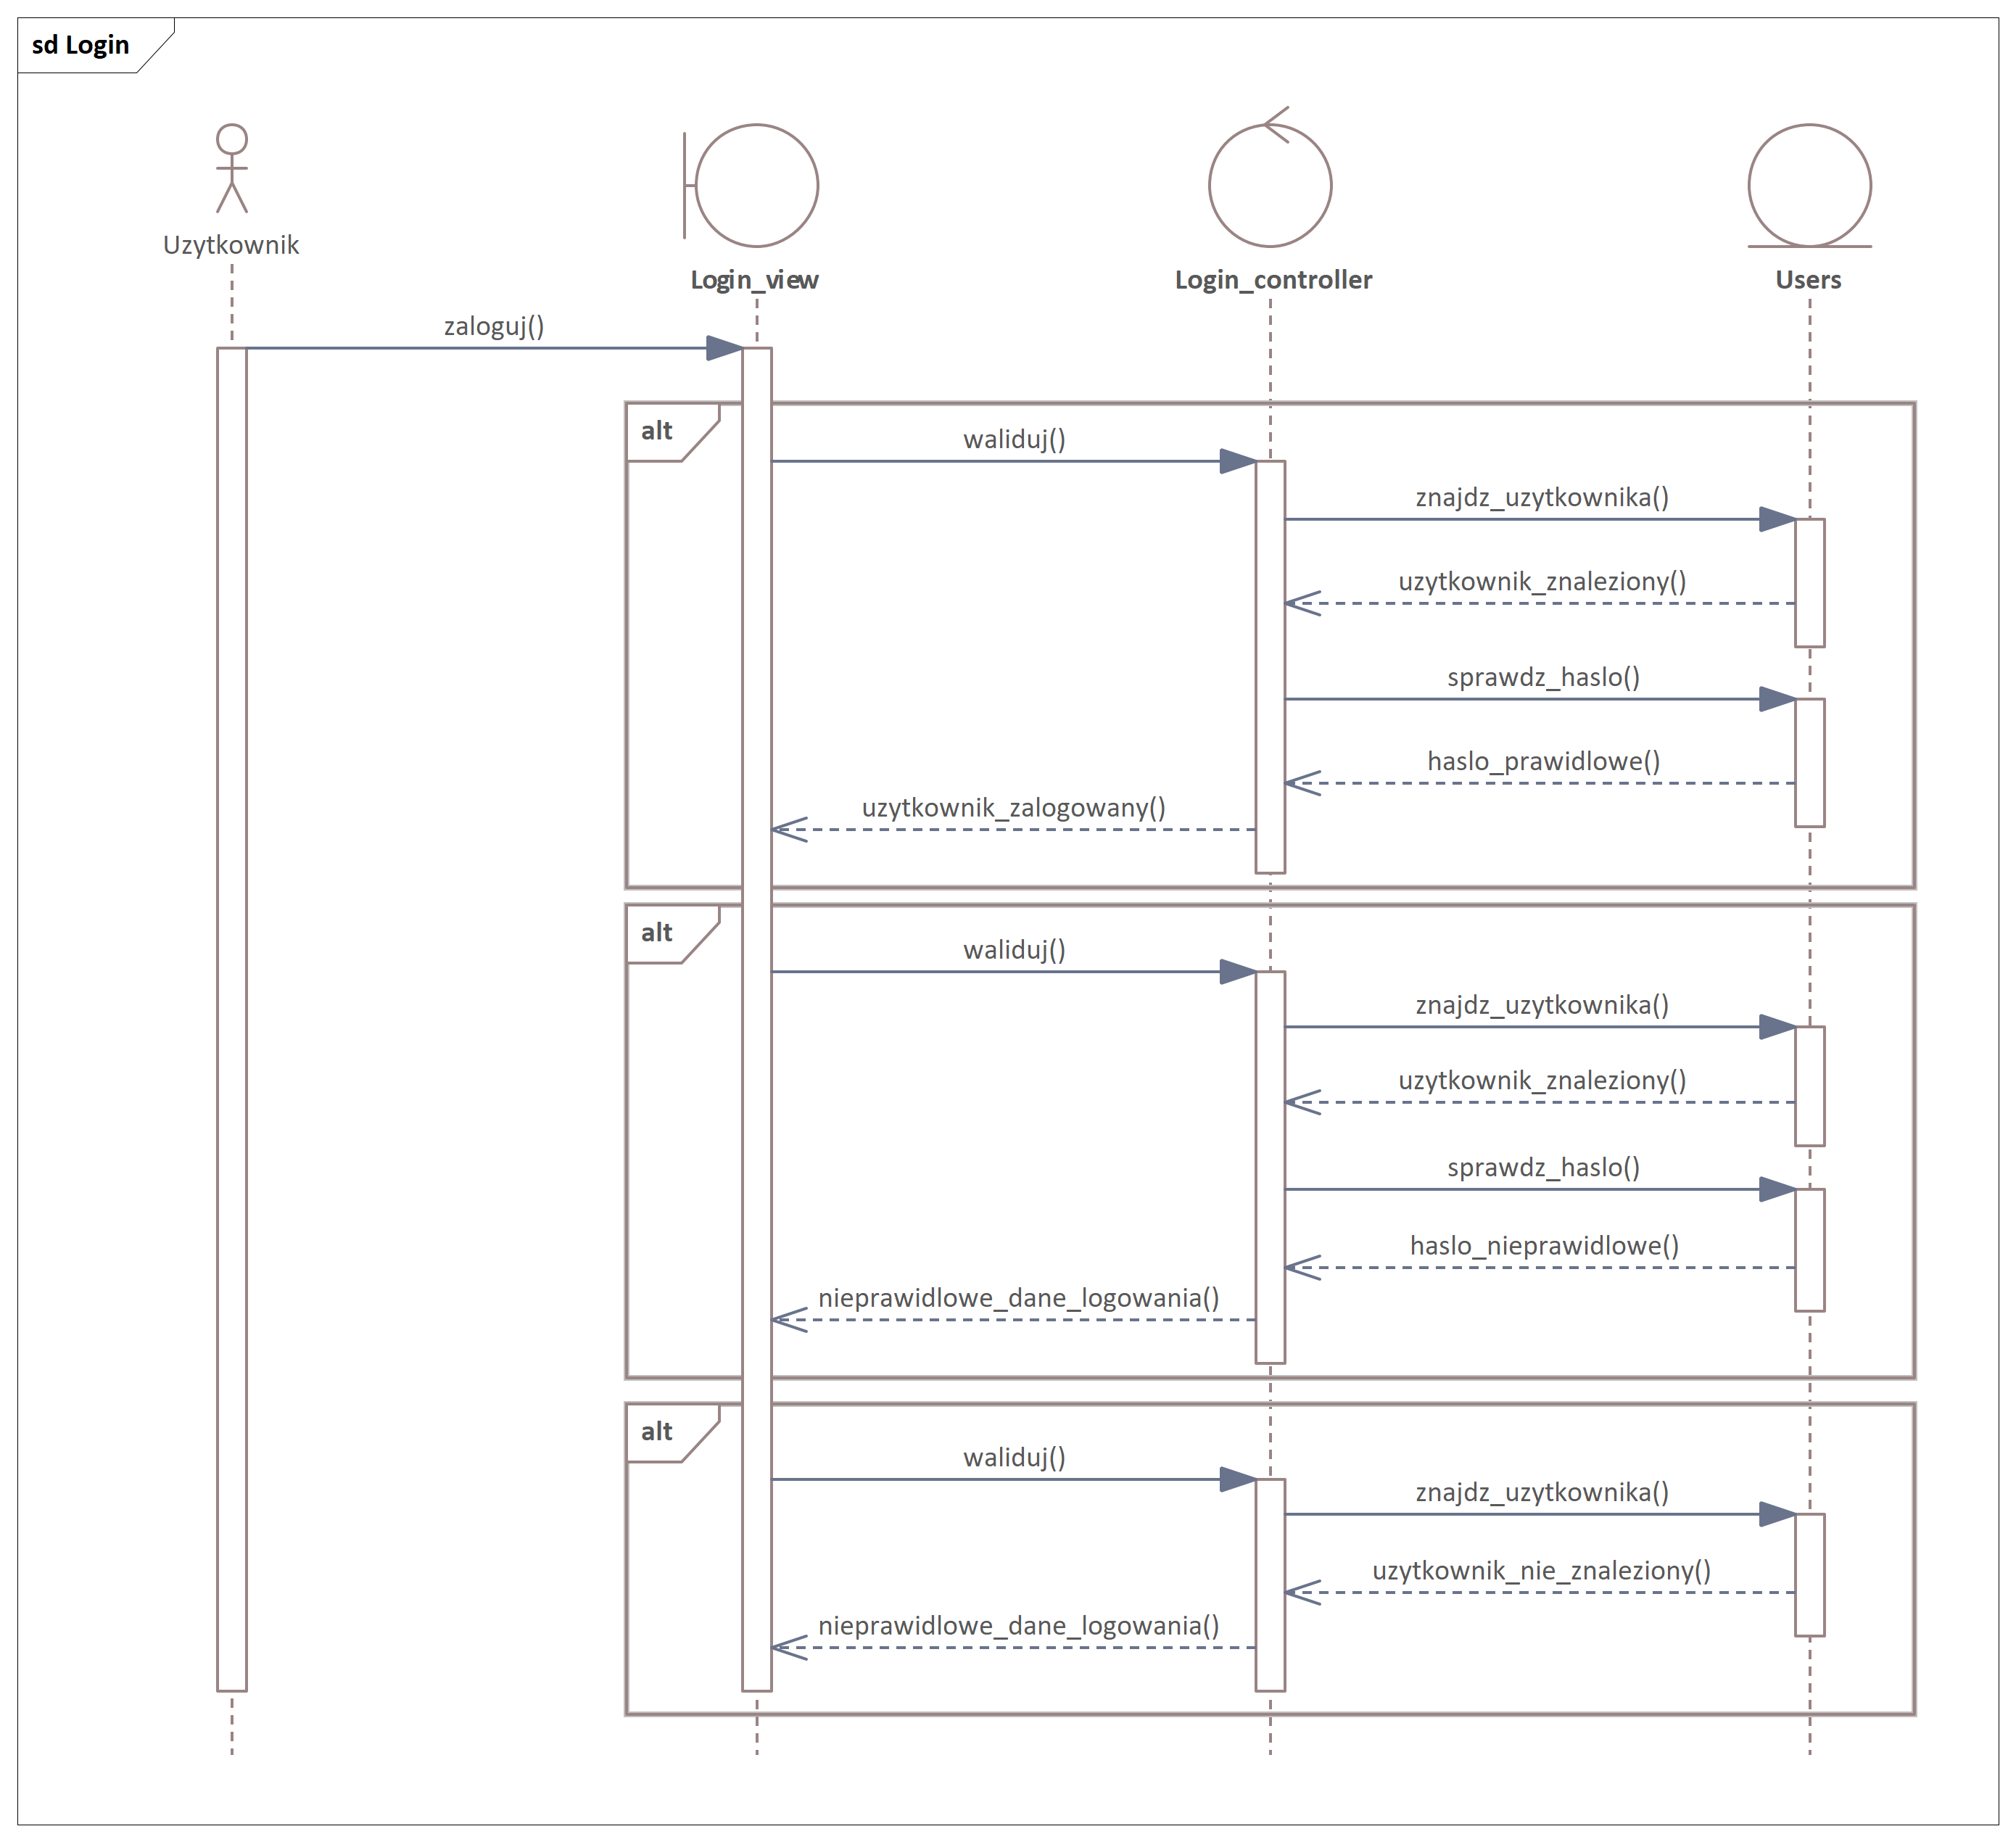
\includegraphics[width=0.8\textwidth]{sprz/sequence_login}
  \caption{Diagram sekwencji dla logowania}
  \label{img:sequence_login}
\end{figure}

Linki \textit{Login} i \textit{Register} są widoczne w pasku menu tylko w razie, gdy żaden użytkownik nie jest zalogowany.

Użytkownicy dzielą się na użytkowników zwykłych oraz na użytkowników z prawami administracyjnymi. W razie zalogowania użytkownika o zwykłych prawach obok przycisku \textit{Logout} pojawia się przycisk z podaną przy logowaniu nazwą użytkownika (\ref{img:app_menu_regular_user}).

\begin{figure}[h]
  \centering
  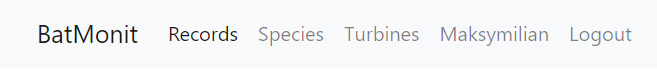
\includegraphics[width=0.8\textwidth]{sprz/app_menu_regular_user}
  \caption{Widok menu dla zwykłego użytkownika}
  \label{img:app_menu_regular_user}
\end{figure}

W przypadku zalogowania użytkownika z prawami administracyjnymi w pasku menu widoczny jest również przycisk \textit{Users} do widoku listy wszystkich istniejących użytkowników (\ref{img:app_users}).

\begin{figure}[h]
  \centering
  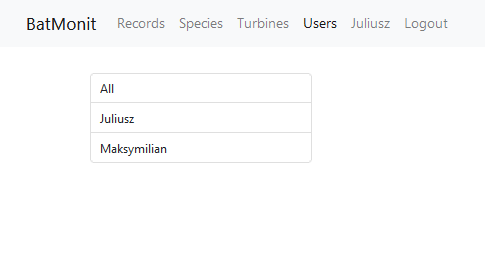
\includegraphics[width=0.8\textwidth]{sprz/app_users}
  \caption{Widok listy użytkowników}
  \label{img:app_users}
\end{figure}

Widok rekordów (\ref{img:app_records}) dzieli się na komponenty odpowiedzialne za filtrowanie wyników w górnej części oraz tabelę wyników w dolnej części.

W górnej części widoku rekordów znajduje się panel filtrów z listą wszystkich gatunków nietoperzy. Kliknięcie na któryś z wymienionych gatunków filtruje listę rekordów i wyświetla tylko rekordy zawierające wybrany gatunek. Domyślny wybór filtrowania to \textit{All}, czyli wyświetlanie wszystkich rekordów.

Poniżej panelu filtrów znajduje się komunikat podsumowujący liczbę istniejących w bazie danych rekordów według aktualnie wybranych kryteriów. W razie braku rekordów do wyświetlenia, w tym miejscu znajduje się komunikat o tej treści.

Pod komunikatem znajduje się okno wyszukiwania, które przyjmuje dane wejściowe od użytkownika i pozwala na wyszukiwanie po zawartości tabeli \textit{Date}.

W nagłówku tabeli zawierającej listę rekordów według aktualnych kryteriów filtrowania znajdują się nazwy poszczególnych kolumn odpowiadających nazwom kolumn w bazie danych. Kliknięcie na nazwie kolumny sortuje wyniki po zawartości tej kolumny w kolejności rosnącej lub malejącej, zaś ponowne kliknięcie odwraca kolejność na przeciwną.

Pod tabelą rekordów znajdują się przyciski paginacji, które pozwalając podzielić listę rekordów na osobne strony i wyświetlić zawartość kolejnych stron. Ilość przycisków stron generowana jest dynamicznie w zależności od ilości rekordów spełniających wybrane kryteria wyszukiwania oraz ilości rekordów wyświetlanych na jednej stronie.

\begin{figure}[h]
  \centering
  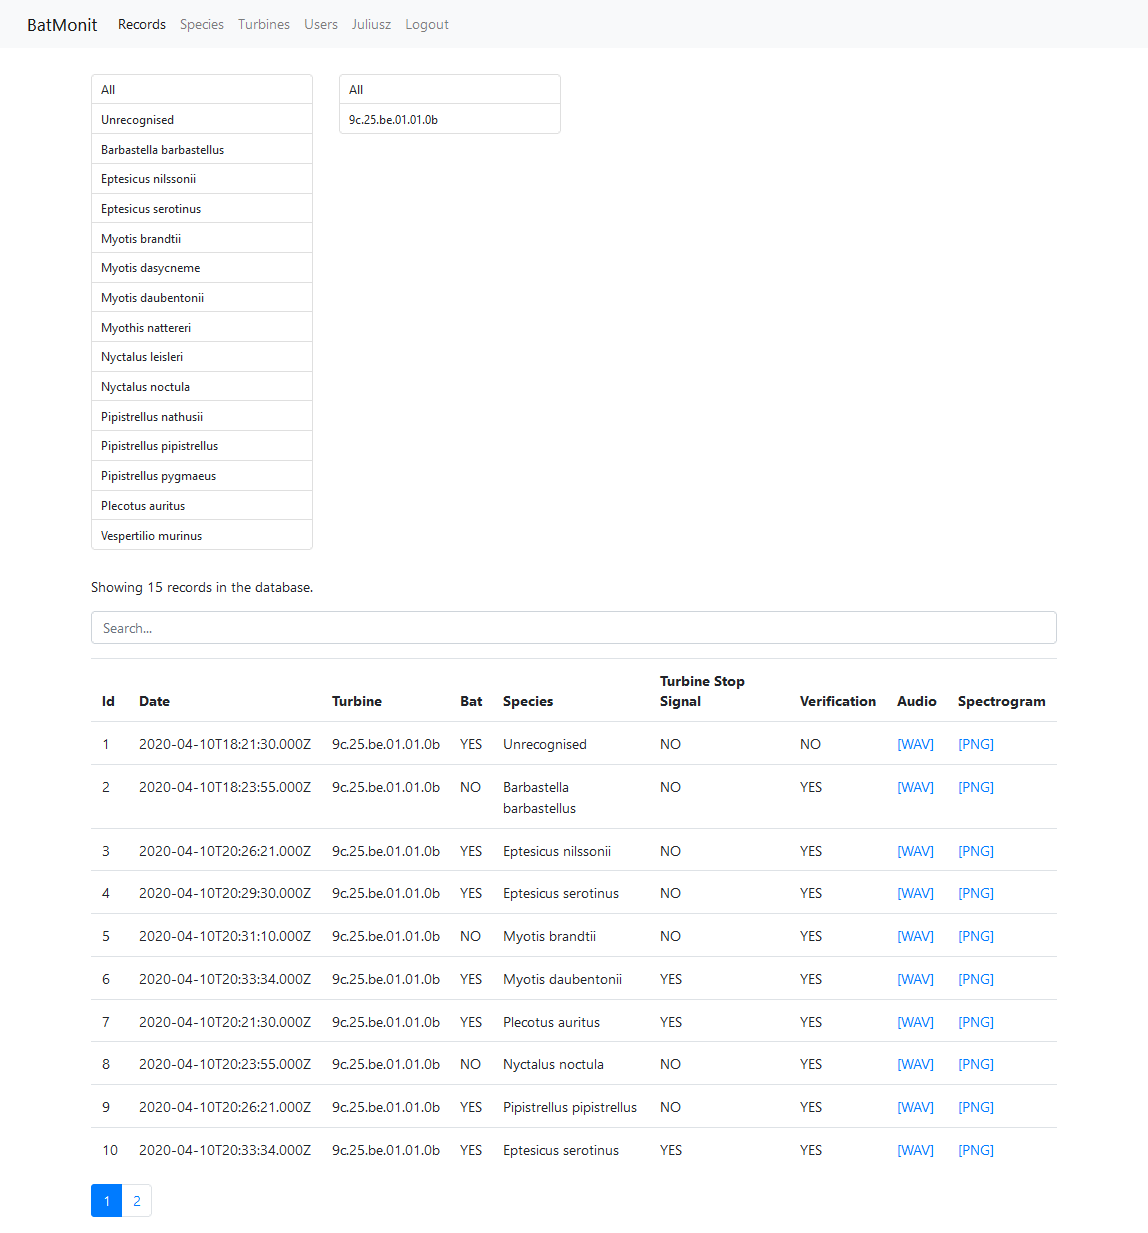
\includegraphics[width=0.8\textwidth]{sprz/app_records}
  \caption{Widok listy rekordów}
  \label{img:app_records}
\end{figure}

Diagram sekwencji wg Rysunku \ref{img:sequence_records} przedstawia logikę działania aplikacji związaną z wyświetlaniem rekordów. W momencie, gdy użytkownik otworzy zakładkę Records z listą rekordów, aplikacja wykonuje zapytanie do bazy danych i pobiera listę rekordów.

\begin{figure}[h]
  \centering
  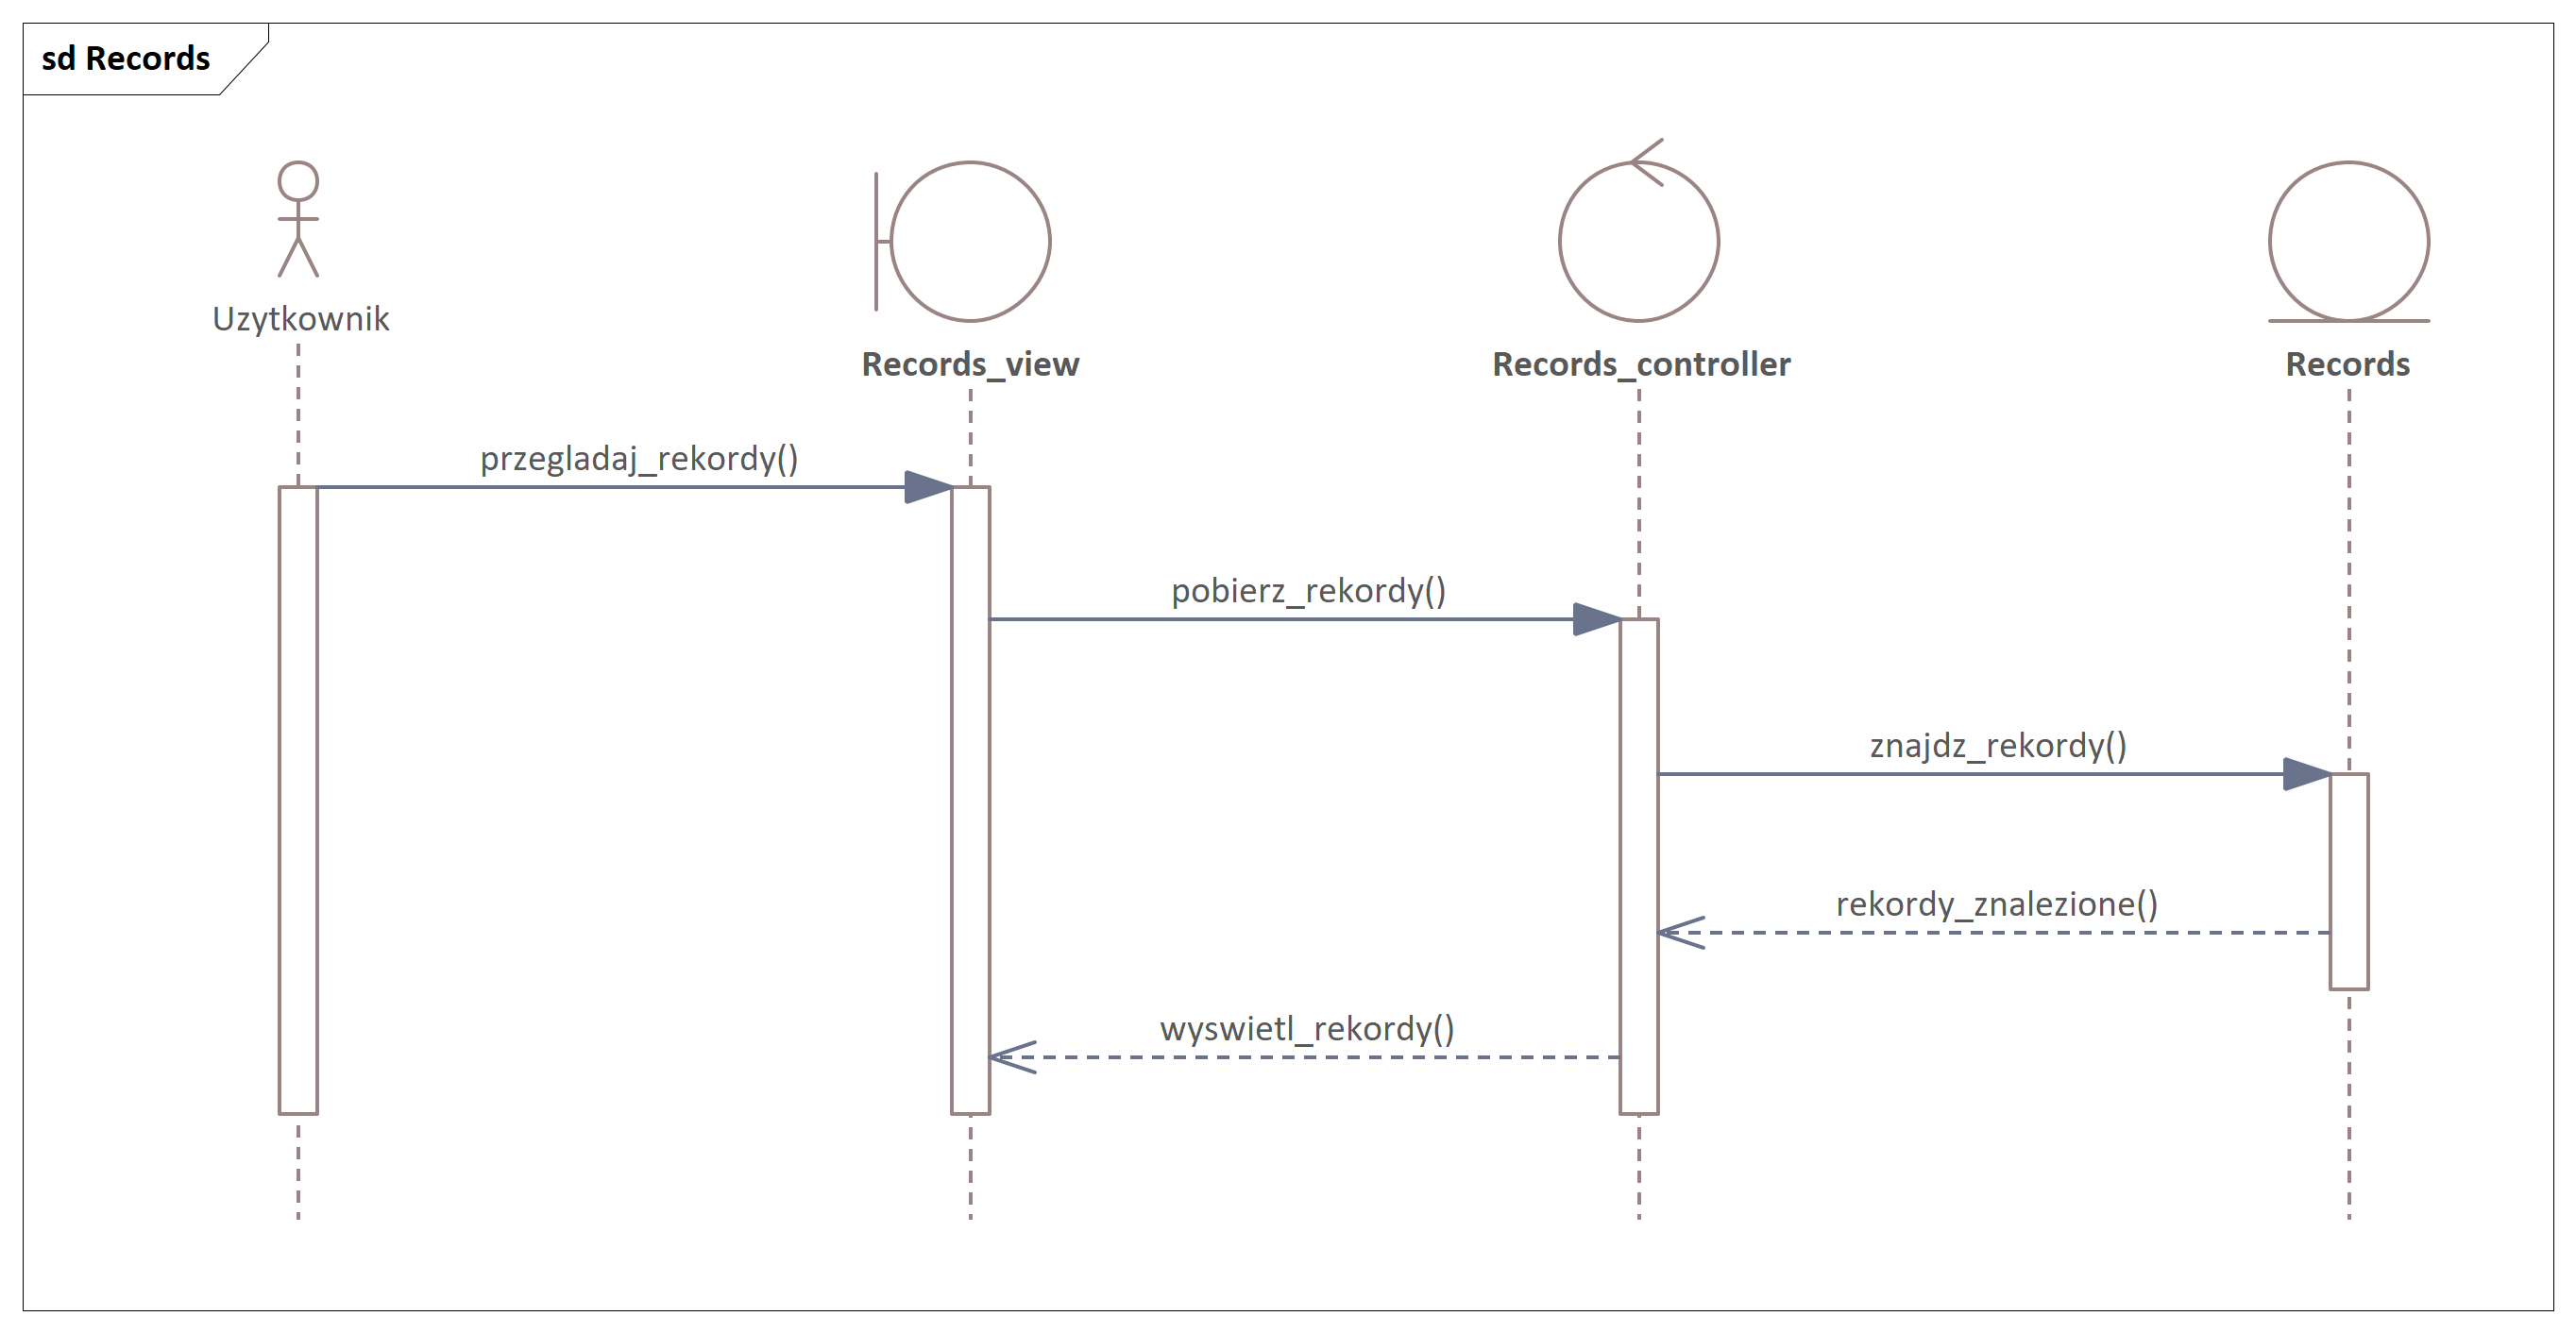
\includegraphics[width=0.8\textwidth]{sprz/sequence_records}
  \caption{Diagram sekwencji dla rekordów}
  \label{img:sequence_records}
\end{figure}

\chapter{Implementacja Watchdoga}

Watchdog jest mikroserwisem do synchronizacji danych z systemu SMART z bazą danych i aplikacją. Jest programem napisanym w języku Python. Stanowi połączenie pomiędzy systemem SMART, a Aplikacją Użytkownika, której przekazuje rekordy zawierające wynik jego pracy. 

W pierwszej kolejności Watchdog monitoruje folder nagrań na wypadek pojawienia się nowego nagrania. Przedstawiono to na Listingu \ref{lst:watch_directory}

\begin{lstlisting}[language=Python,caption={Funkcja służąca do monitorowania folderu z nagraniami}, label={lst:watch_directory}]
  def watch_directory():
  from watchdog.events import FileSystemEventHandler
  from watchdog.observers import Observer

  class MyHandler(FileSystemEventHandler):
      def on_created(self, event):
          if event.is_directory:
              return
          file_name = os.path.basename(event.src_path)
          print(f'Utworzono plik: {file_name}')
          record = NewRecord(file_name)
          create_record(vars(record))

  event_handler = MyHandler()
  observer = Observer()
  observer.schedule(event_handler, PATH, recursive=True)
  observer.start()
  print("Watchdog is watching...")
  try:
      while True:
          time.sleep(1)
  except KeyboardInterrupt:
      observer.stop()
  observer.join()
  \end{lstlisting}

Pojawienie się nowego pliku wywołuje zdarzenie, które powoduje, że wykonany zostaje kod parsujący nazwę pliku. Nazwa pliku nagrania zapisana jest w formacie, który przedstawia Listing \ref{lst:recording_name}.

\begin{lstlisting}[language=Java,caption={Przykładowa nazwa pliku nagrania}, label={lst:recording_name}]
  9c.25.be.01.01.0b_20240123_225004_701432.wav
\end{lstlisting}

Nazwa pliku podzielona jest na cztery człony oddzielone znakiem ” ” i zakończone rozszerzeniem pliku WAV. Pierwszy człon odnosi się do identyfikatora konkretnego urządzenia SMART. Drugi człon to data nagrania w formacie YYYYMMDD. Trzeci człon to czas nagrania w formacie HHMMSS. Ostatni człon jest losową sześciocyfrową liczbą. Po wyodrębnieniu powyższych członów zostają one zapisane do zmiennych.


Następnie Watchdog wykorzystuje model sztucznej inteligencji w celu przeanalizowania pliku nagrania. Analiza nadaje odpowiednią wartość zmiennym bat, turbineStopSignal oraz verification. W kolejnym kroku zapisane zmienne zostają umieszczone wewnątrz obiektu JSON (JavaScript Object Notation). Obiekt JSON za pomocą metody POST zostaje wysłany na adres API serwera.
Serwer nasłuchuje na porcie ”http://localhost:3900/api/records” i po pojawieniu się zapytania z obiektem JSON tworzy na jego podstawie rekord w bazie danych

\clearpage

\chapter{Implementacja aplikacji użytkownika}

Aplikacja użytkownika służy do zbierania i zapisywania w bazie danych rekordów tworzonych na podstawie decyzji modelu sieci neuronowej, które następnie pozwala wyświetlić na liście z możliwością filtrowania i sortowania ich. W skład aplikacji wchodzą: baza danych, serwer oraz interfejs użytkownika.

Centralną rolę pełni serwer, który pośredniczy w komunikacji z bazą danych i przyjmuje komunikację ze strony modelu sztucznej inteligencji oraz interfejsu użytkownika. Komunikacja ta realizowana jest poprzez interfejs API (Application Programming Interface).
\clearpage

\section{Baza danych}

Wybrana przez autorów projektu technologia bazy danych to MySQL. Jest to jeden z najbardziej rozpowszechnionych systemów relacyjnych baz danych. Do jego zalet należy szeroka obsługa platform i architektur.

Baza danych zawiera tabele \verb|records|, \verb|turbines|, \verb|species| oraz \verb|users|. Tabela\verb|users| gromadzi dane zarejestrowanych użytkowników i nie ma relacji z pozostałymi tabelami (\ref{img:db_diagram}).

\begin{figure}[h]
  \centering
  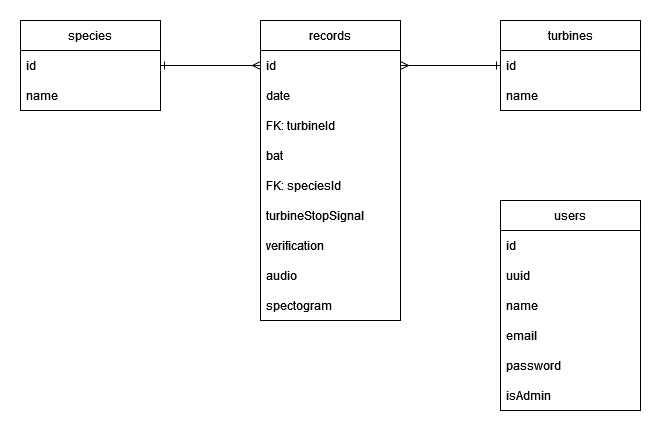
\includegraphics[width=0.8\textwidth]{sprz/db_diagram}
  \caption{Diagram bazy danych}
  \label{img:db_diagram}
\end{figure}

\section{NodeJS}

Serwer aplikacji został napisany w technologii NodeJS \cite{nodejs}. Technologia ta charakteryzuje się relatywnie niskim progiem wejścia do tworzenia oprogramowania i otwiera programistom pracującym nad frontendem w języku Javascript na wykorzystanie swojej wiedzy w tym języku przy pracy w backendzie. Jednocześnie na ujednolicenie pod względem języka oprogramowania części backendowej i frontendowej. Dzięki temu dobrze nadaje się do zastosowania w niniejszym projekcie.

NodeJS to wieloplatformowe środowisko składające się z V8 (silnika Javascript firmy Google), pętli zdarzeń obsługiwanej przez bibliotekę libUV oraz interfejsu do obsługi niskopoziomowego wejścia-wyjścia.

Do zalet NodeJS należy:
\begin{enumerate}
  \item \textbf{Asynchroniczność.} Poprzez nieblokującą obsługę wejścia-wyjścia służy do tworzenia wysoce skalowalnych rozwiązań serwerowych przy maksymalizacji wykorzystania procesora i pamięci.
  \item \textbf{Wysoka skalowalność.} Pętla zdarzeń pozwala uniknąć tworzenia wielowątkowych rozwiązań. Procesy mogą być uruchamiane współbieżnie lub równolegle. Wywołanie zwrotne (ang. callback) sygnalizuje następnie powodzenie lub niepowodzenie zadania.
  \item \textbf{Duża popularność.} Dostępne są tysiące bibliotek o otwartym kodzie źródłowym tworzonych przez środowisko NodeJS.
\end{enumerate}

\section{Biblioteki}

W projekcie użyto następujących otwartych bibliotek, które dostarczyły szeregu funkcjonalności i skróciły czas jego tworzenia:
\begin{itemize}
  \item Sequelize
  \item Express
  \item Joi
  \item Jsonwebtoken
\end{itemize}

\subsection*{Sequelize}

Do komunikacji z bazą danych wykorzystano bibliotekę Sequelize \cite{sequelize}. Sequelize to narzędzie mapowania obiektowo-relacyjnego (ang. ORM - Object-Relational Mapping), które pełni rolę "pomostu" pomiędzy aplikacją obiektową a relacyjną bazą danych.
Do zalet ORM należą:
\begin{itemize}
  \item odwzorowanie tabel relacyjnej bazy danych na obiekty w obiektowym języku programowania wykorzystanym w aplikacji
  \item wykonywanie operacji na danych w bazie danych jak na obiektach języka programowania
  \item uniknięcie nadmiarowego kodu
  \item wykorzystanie tego samego kodu aplikacji w komunikacji z różnymi bazami danych
  \item tworzenie zapytań dla wielu tabel
  \item przyspieszenie i uproszczenie procesu wytworzenia aplikacji
\end{itemize}

Biblioteka ta pozwoliła na wyeliminowanie w kodzie potrzeby formułowania zapytań w języku SQL, które jest trudne w utrzymaniu z punktu widzenia programisty i podatne na błędy w treści zapytań. Serwer posiada zdefiniowany model odpowiadający każdej tabeli w bazie danych. Na podstawie modelu biblioteka Sequelize ma informacje potrzebne do stworzenia zapytania w języku SQL. Listing \ref{lst:Sequelize_Record.create} przedstawia przykład przekazania szeregu zmiennych w celu zapisania ich jako nowy rekord w bazie danych.

\begin{lstlisting}[language=Java,caption={Przykład tworzenia rekordu z pomocą biblioteki Sequelize}, label={lst:Sequelize_Record.create}]
  const record = await Record.create({
    date,
    turbineId,
    bat,
    speciesId,
    turbineStopSignal,
    verification,
    audio,
    spectrogram,
  });
\end{lstlisting}

Biblioteka Sequelize oferuje wbudowaną walidację zapytań po zdefiniowanych w modelu typach danych. Istnieje również możliwość tworzenia niestandardowych komunikatów w razie błędu wykrytego przez walidację, co ukazuje listing \ref{lst:Sequelize_validate}.

\begin{lstlisting}[language=Java,caption={Przykład niestandardowego komunikatu walidacji}, label={lst:Sequelize_validate}]
  Record.init(
    {
      date: {
        type: DataTypes.DATE,
        allowNull: false,
        validate: {
          notNull: { msg: "Record must have a date" },
          notEmpty: { msg: "Date must not be empty" },
        },
      },
    }
  );
\end{lstlisting}

Iteracyjne tworzenie projektu programistycznego z relacyjną bazą danych niesie ze sobą duże ryzyko wprowadzenia zmian do bazy danych, które uszkodziłyby jej strukturę i mogłyby doprowadzić do utraty danych. Takie błędne zmiany są trudne to rozpoznania i usunięcia. Biblioteka Sequelize wychodzi na przeciw potrzebie minimalizacji ryzyka przy zmianach w bazie danych poprzez uwzględnianie ich wewnątrz migracji, podobnie do rozwiązań stosowanych w środowisku korporacyjnym (takich jak Hibernate/Liquibase w projektach w języku Java).

Migracja Sequelize jest to funkcja Javascript zawierająca metodę \textit{up} zawierającą kod zmieniający bazę danych oraz metodę \textit{down} specyfikujący kod odwracający zmiany z metody \textit{up}. Migracja jest zawarta wewnątrz pojedynczego pliku o unikalnej nazwie zawierającej datę utworzenia i opis wprowadzanych zmian. Pliki takie biblioteka Sequelize pozwala tworzyć poleceniem w konsoli. Ideą zastosowania migracji jest stworzenie tym sposobem systemu kontroli wersji dla zmian w bazie danych. Każde zmiany w bazie danych powinny zostać poprzedzone utworzeniem pliku migracji i wypełnieniem obu metod. W razie wystąpienia problemów z bazą danych biblioteka Sequelize pozwala za pomocą konsoli na cofanie się w historii zmian i przywrócenie poprzedniego stanu. Przykład migracji ukazuje listing \ref{lst:Sequelize_migration}.

\begin{lstlisting}[language=Java,caption={Przykład pliku migracji}, label={lst:Sequelize_migration}]
  module.exports = {
    async up(queryInterface, DataTypes) {
      await queryInterface.createTable("records", {
        id: {
          allowNull: false,
          autoIncrement: true,
          primaryKey: true,
          type: DataTypes.INTEGER,
        },
      });
    },
    async down(queryInterface, DataTypes) {
      await queryInterface.dropTable("records");
    },
  };
\end{lstlisting}

O ile zmiany w strukturze tabel bazy danych zarządzane są przez migracje, biblioteka Sequelize daje również możliwość masowego zapełniania bazy danych danymi. Jest to szczególnie przydatne przy procesie implementacji. Pozwala na przyspieszenie i zautomatyzowanie procesu operowania danymi testowymi oraz eliminuje potrzebę bezpośredniego wykonywania zapytań w narzędziu zarządzającym bazą danych (jak np. MySQL Workbench). Do tego celu służą pliki seeder, które w istocie są podobne do migracji, lecz w metodach \textit{up} i \textit{down} należy zawierać kod operujący na danych, nie zaś na strukturze tabel bazy danych. Przykład migracji ukazuje listing \ref{lst:Sequelize_seeder}.

\begin{lstlisting}[language=Java,caption={Przykład pliku seeder}, label={lst:Sequelize_seeder}]
  module.exports = {
    async up(queryInterface, Sequelize) {
      await queryInterface.bulkInsert(
        "turbines",
        [
          {
            name: "9c.25.be.01.01.0b",
            createdAt: "2022-07-27 21:04:11",
            updatedAt: "2022-07-27 21:04:11",
          },
        ],
        {}
      );
    },
  
    async down(queryInterface, Sequelize) {
      await queryInterface.bulkDelete("turbines", null, {});
    },
  };
\end{lstlisting}

\subsection*{Express}

Serwer w NodeJS do komunikacji z modelem w celu stworzenia rekordów oraz pośredniczenia z interfejsem użytkownika w odczytywaniu zapisanych rekordów wykorzystuje interfejsu API stworzonego z pomocą biblioteki Express \cite{express}.

Biblioteka Express to szablon (ang. framework) dostarczający mechanizmy do:
\begin{itemize}
  \item pisania zapytań HTTP dla różnych ścieżek URL (ang. Uniform Resource Locator)
  \item generowania widoków przez wstawianie danych do modelu
  \item definiowania ogólnych ustawień w aplikacji, jak np. port wykorzystywany do połączenia lub model wykorzystywany do renderowania odpowiedzi
  \item dodawania na dowolnym etapie przetwarzania zapytania wywołania oprogramowania pośredniczącego (ang. middleware)
\end{itemize}

Biblioteka Express pozwoliła na uporządkowanie i czytelne rozmieszczenie zaprogramowanych interfejsów API w imię zasady pojedynczej odpowiedzialności.

\subsection*{Joi}

Do walidacji treści wpisywanej przez użytkownika aplikacji przy rejestracji lub logowaniu posłużyła biblioteka Joi. Dostarcza ona wygodny i czytelny szablon tworzenia warunków walidacyjnych. W razie ich niespełnienia przez walidowaną treść któregoś z warunków, zwracany jest błąd o określonej treści. W odróżnieniu od walidacji oferowanej przez bibliotekę Sequelize, Joi pozwala na walidację bardziej wysokopoziomową i nie jest wiązana modelem tworzącym bazę danych.

Listing \ref{lst:Joi} przedstawia wykorzystanie biblioteki Joi wewnątrz funkcji pośredniczącej do potwierdzania tożsamości użytkownika.

\begin{lstlisting}[language=Java,caption={Przykład wykorzystania Joi}, label={lst:Joi}]
  function validate(req) {
    const schema = Joi.object({
      email: Joi.string().min(5).max(255).required().email(),
      password: Joi.string().min(5).max(255).required(),
    });
  
    return schema.validate(req);
  }
\end{lstlisting}

\subsection*{Jsonwebtoken}

Biblioteka Jsonwebtoken dostarcza metody to generowania i walidowania tzw. tokenów, czyli zaszyfrowanych kluczy. Po udanym logowaniu użytkownika generowany i przesyłany wewnątrz odpowiedzi jest token. Następnie token ten przechowywany jest przez przeglądarkę i dodawany do kolejnych zapytań w komunikacji między interfejsem użytkownika a serwerem poprzez interfejs API. Serwer sprawdza za każdym razem, czy przychodzące zapytanie posiada właściwy token, a w przeciwnym wypadku odmawia przesłania odpowiedzi.

\section{ReactJS}

Interfejs użytkownika został napisany w języku Javascript przy wykorzystaniu biblioteki ReactJS, jednej z najbardziej popularnych bibliotek do tworzenia interfejsów graficznych.

Stosowanie biblioteki ReactJS oferuje wiele korzyści:
\begin{enumerate}
  \item \textbf{Tworzenie dynamicznych aplikacji internetowych.} Wymaga napisania mniejszej ilości kodu i oferuje więcej funkcjonalności w odróżnieniu do pracy z samym językiem Javascript.
  \item \textbf{Lepsza wydajność.} Wykorzystując wirtualny DOM (ang. Document Object Model) pozwala na porównywanie poprzedniego stanu każdego komponentu i odświeżanie tylko tych komponentów, które uległy zmianie, w przeciwieństwie do odświeżania wszystkich komponentów. Dzięki temu aplikacje stworzone w ReactJS są bardziej responsywne, szybciej się ładują. Na przykład, ReactJS pozwala na proste korzystanie w tworzonym interfejsie graficznym z asynchroniczności, w której reakcja na akcję użytkownika może być natychmiastowa, a komponent oczekujący na dane nie wstrzymuje aplikacji i wyświetli je, kiedy tylko je otrzyma.
  \item \textbf{Komponenty wielokrotnego użytku.} Aplikacja w ReactJS składa się z wielu komponentów. Każdy z nich posiada logikę, która może zostać wielokrotnie wykorzystana w innym miejscu aplikacji, co pozwala na skrócenie czasu tworzenia aplikacji. Ponadto, podział na komponenty pozwala na funkcjonalne uporządkowanie kodu i poprawienie jego czytelności.
  \item \textbf{Jednokierunkowy przepływ danych.} ReactJS przestrzega jednokierunkowego przepływu danych. Oznacza to, że dane są przekazywane tylko w dół hierarchii od komponentów nadrzędnych do dziedziczących. Widok aplikacji jest rezultatem stanu danych. Stan danych zmienia się pod wpływem akcji. Gdy następują akcje, stan zostaje odświeżony. W rezultacie łatwiejsze staje się unikanie oraz poszukiwanie błędów w kodzie.
  \item \textbf{Szybsze wdrożenie się.} ReactJS pozwala mniej doświadczonym programistom na relatywnie szybki start przy tworzeniu zaawansowanych dynamicznych aplikacji.
  \item \textbf{Ciągły rozwój i popularność.} ReactJS z uwagi na swoją popularność posiada dużą społeczność użytkowników, co skutkuje szeroką dostępnością materiałów edukacyjnych oraz bogatym wsparciem technicznym.
\end{enumerate}

W okresie powstawania niniejszej aplikacji nastąpiły zmiany w obowiązujących trendach odnośnie rodzaju wykorzystywanych komponentów. Z początku w środowisku ReactJS panowała tendencja do stosowania komponentów klasowych \ref{lst:class_component}, czyli programowania obiektowo w sposób zaczerpnięty z obiektowych języków programowania, takich jak np. Java. Komponent klasowy jest klasą dziedziczącą po klasie Component. Posiada stan, akcje, które wpływają na stan, oraz metody cyklu życia (ang. lifecycle methods). Metody cyklu życia zawierają kod, który ma się wykonać przy uruchomieniu (componentDidMount), odświeżeniu (componentDidUpdate) lub zamknięciu (componentWillUnmount) komponentu.

\begin{lstlisting}[language=Java,caption={Przykład komponentu klasowego}, label={lst:class_component}]
  class Records extends Component {
    state = {
      records: [],
      turbines: [],
      species: [],
      currentPage: 1,
      pageSize: 8,
      selectedSpecies: null,
      selectedTurbine: null,
      searchQuery: "",
      sortColumn: { path: "title", order: "asc" },
    };
  
    async populateSpecies() {
      const { data } = await getSpecies();
      const species = [{ id: "", name: "All" }, ...data];
      this.setState({ species });
    }

    async componentDidMount() {
      await this.populateSpecies();
      await this.populateTurbines();
      await this.populateRecords();
    }
  }
\end{lstlisting}

Do zastosowań nie wymagających śledzenia stanu komponentu służył bezstanowy komponent funkcjonalny \ref{lst:stateless_functional_component}, który w zasadzie zwraca tylko kod JSX będący wykorzystaniem znaczników HTML wewnątrz kodu Javascript. Jest to wygodne rozwiązanie do minimalistycznego i czytelnego programowania widoków, szczególnie do wykorzystania w wielu miejscach z innymi danymi przekazanymi do komponentu w formie argumentów.

\begin{lstlisting}[language=Java,caption={Przykład bezstanowego komponentu funkcjonalnego}, label={lst:stateless_functional_component}]
  const input = ({ name, label, error, ...rest }) => {
    return (
      <div className="form-group">
        <label htmlFor={name}>{label}</label>
        <input {...rest} name={name} id={name} className="form-control" />
        {error && <div className="alert alert-danger">{error}</div>}
      </div>
    );
  }
\end{lstlisting}

W ReactJS wraz z wersją 16.8 wprowadzono możliwość śledzenia stanu wewnątrz komponentów funkcjonalnych \ref{lst:functional_component}. Sprawiło to, że komponenty funkcjonalne stały się równoważne do komponentów klasowych pod względem oferowanych funkcjonalności, lecz zachowały dotychczasową przewagę pod względem prostoty do wykorzystania i czytelności kodu. W komponencie funkcjonalnym metoda useEffect pełni funkcję metod cyklu życia komponentu klasowego. Stan komponentu przechowywany jest w zmiennych. Każdej zmiennej stanu komponentu odpowiada według konwencji metoda o tej samem nazwie z przedrostkiem \textit{set}, która pełni funkcję settera. Stan początkowy zmiennych stanu inicjowany jest przez metodę useState.

\begin{lstlisting}[language=Java,caption={Przykład komponentu funkcjonalnego}, label={lst:functional_component}]
  export default function Species() {
    const [species, setSpecies] = useState([]);
    const [selectedSpecies, setSelectedSpecies] = useState([]);
  
    useEffect(() => {
      async function fetchData() {
        const { data } = await getSpecies();
        const species = [{ id: "", name: "All" }, ...data];
        setSpecies(species);
      }
      fetchData();
    }, []);
  
    function handleSpeciesSelect(species) {
      setSelectedSpecies(species);
    }
  }
\end{lstlisting}

Z uwagi na wspomniane zalety komponentów funkcjonalnych posiadających stan obecnie zalecane jest stosowanie komponentów funkcjonalnych zamiast klasowych w nowych projektach pisanych w ReactJS. Dostępne są również dobrze opisane materiały pomagające w migracji istniejącego kodu do komponentów funkcjonalnych \cite{react-component}.

\chapter{Testowanie}

\section{Testy terenowe systemu SMART}
Mikrofon ultradźwięków wraz z kontrolerem działały nieprzerwanie od dnia montażu do dnia 30.01.2024. do godz. 7:30, rejestrując w tym czasie łącznie 42,44 GB danych, w tym 44 915 plików WAV.
Zdolność mikrofonu do rejestracji sztucznie wytworzonych głosów nietoperzy została zaprezentowana w rozdziale "Prace badawczo-rozwojowe - testy terenowe".

\section{Testy oprogramowania}
Przygotowano trzy rodzaje testów oprogramowania - testy jednostkowe, testy integracyjne i testy systemowe. Testy jednostkowe są klasycznie implementowanymi testami podczas wytwarzania oprogramowania i miały na celu sprawdzenie poprawności działania niewielkich elementów oprogramowania. Testy integracyjne i systemowe posłużyły z kolei do sprawdzenia poprawności działania systemu w większej skali, na poziomie całego systemu oraz poszczególnych funkcji, które zdefiniowano uprzednio dla systemu.

\subsection{Testy jednostkowe}

Za szablon do pisania testów jednostkowych (ang. unit test) posłużyła biblioteka Jest. Jest to popularna biblioteka do testowania rozwiązań w języku Javascript, dostarczająca szablony pisania testów i metody asercji. Dodatkowo biblioteka ta dostarcza narzędzia do analizy i wygenerowania raportu procentowego stopnia pokrycia testami (ang. test coverage) całego kody aplikacji. Pozwala w ten sposób łatwo ustalić, które części aplikacji wymagają jeszcze utworzenia testów. Rysunek (\ref{img:test_coverage}) ukazuje przykładowy raport pokrycia testami.

\begin{figure}[h]
  \centering
  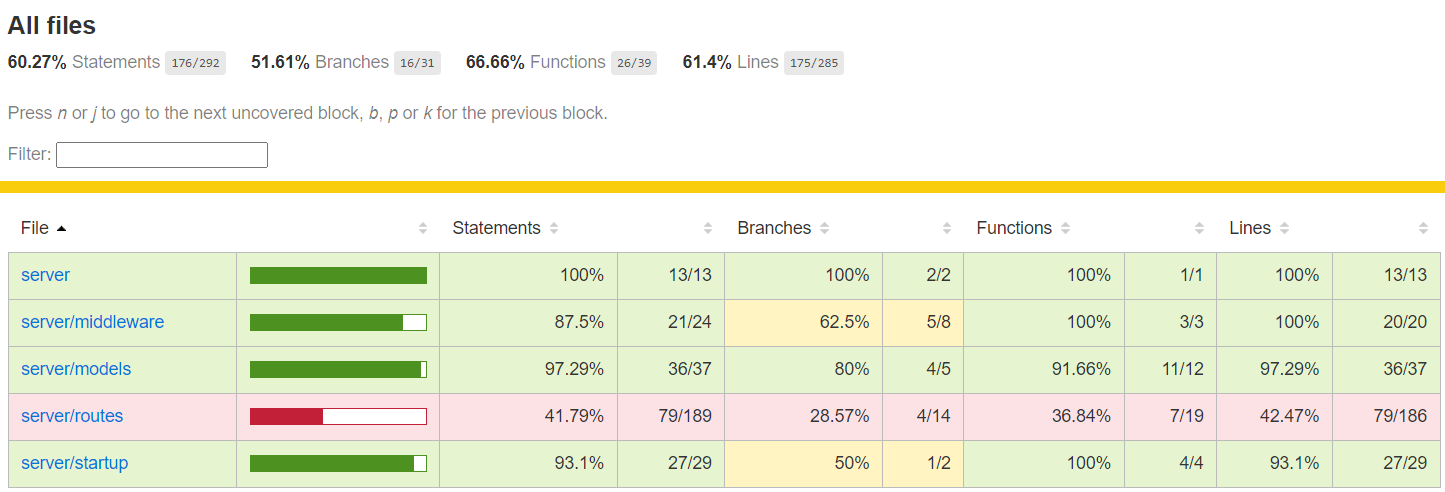
\includegraphics[width=0.8\textwidth]{sprz/test_coverage}
  \caption{Przykładowy raport pokrycia testami}
  \label{img:test_coverage}
\end{figure}

Listing \ref{lst:Jest_unit_test} przedstawia przykład testu jednostkowego z wykorzystaniem biblioteki Jest.

Metoda \textit{describe} pozwala podzielić testy na zestawy odpowiadające konkretnej funkcjonalności. Metoda \textit{it} definiuje pojedynczy przypadek testowy, a sama jej nazwa czytana w języku angielskim nakierowuje na zgodne z konwencją nazywanie przypadku testowego w formie słownego opisu spodziewanego wyniku.

\begin{lstlisting}[language=Java,caption={Test jednostkowy z wykorzystaniem Jest}, label={lst:Jest_unit_test}]
  describe("auth middleware", () => {
    it("should populate req.user with the payload of a valid JWT", () => {
      const user = {
        uuid: new DataTypes.UUIDV4(),
        name: "Username",
        isAdmin: true,
      };
      const token = generateAuthToken(user);
      const req = {
        header: jest.fn().mockReturnValue(token),
      };
      const res = {};
      const next = jest.fn();
  
      auth(req, res, next);
  
      expect(req.user).toMatchObject(user);
    });
  });
\end{lstlisting}

\subsection{Testy integracyjne}

Biblioteka Supertest w połączeniu z biblioteką Jest posłużyła do utworzenia testów integracyjnych. W projekcie posłużyła ona do testowania działania interfejsów API.

Listing \ref{lst:Supertest} przedstawia przykład testu integracyjnego z wykorzystaniem biblioteki Jest. Dostarczana przez bibliotekę Jest metoda \textit{beforeEach} zawiera kod wykonywany przed każdym przypadkiem testowym, zaś metoda \textit{afterEach} po każdym przypadku testowym.

\begin{lstlisting}[language=Java,caption={Test integracyjny z wykorzystaniem Supertest i Jest}, label={lst:Supertest}]
  describe("/api/records", () => {
    beforeEach(async () => {
      server = require("../../index");
    });
    afterEach(async () => {
      await server.close();
      await Record.truncate();
    });
  
    describe("GET /", () => {
      it("should return all records", async () => {
        const res = await request(server).get("/api/records");
  
        expect(res.status).toBe(200);
      });
    });
  });
\end{lstlisting}

\subsection{Testy funkcjonalne}
W ramach testów sprawdzono zgodność sytemu z wymaganiami Klienta Wewnętrznego (Dziekan, Promotor) i Zewnętrznego (przedstawiciele Bioseco S.A., przedstawiciele klientów Bioseco S.A.). Wymagania te zostały wymienione i opisane poniżej. Sposób przeprowadzenia testów został opisany przy poszczególnych funkcjach systemu. Były one realizowane poprzez sprawdzenie systemu w działaniu.

\subsubsection{Rejestracja ultradźwięków}
Rejestracja ultradźwięków została przetestowana w trakcie testów terenowych systemu SMART z wykorzystaniem sztucznie wytworzonych ultradźwięków. Zostało to opisane w punktach: "Testy terenowe systemu SMART" oraz "Prace badawczo-rozwojowe - testy terenowe". 

Z testów tych wynika, że system wykrywał większość odtworzonych dźwięków o danej częstotliwości, jeśli dźwięk taki na danej odległości od mikrofonu był wykrywany. Tylko w dwóch przypadkach zarejestrowano 66\% odtworzonych dźwięków (2 na 3 odtworzone dźwięki - obydwa przypadki były dla odległości 40 m i częstotliwości 25-35 kHz, pierwszy dla kąta 30\textdegree, a drugi dla kąta 60\textdegree ), a w jednym przypadku 33\% odtworzonych dźwięków (1 na 3 odtworzone dźwięki, na odległości 20 m od mikrofonu dla częstotliwości 40-48 kHz i przy kącie 0\textdegree).

Ponadto maksymalne odległości detekcji nietoperzy odzywających się w poszczególnych zakresach częstotliwości odpowiadają odległościom obliczonym matematycznie dla tych częstotliwości \cite{agranat}. 

Powyższe dane pozwalają ocenić, że system SMART (mikrofon ultradźwięków wraz z kontrolerem) rejestruje nietoperze z dużą skutecznością, a więc funkcjonalność rejestracji nietoperzy jest zrealizowana.

\subsubsection{Rejestracja ultradźwięków 360\textdegree dookoła turbiny wiatrowej}
W celu realizacji tej funkcjonalności zostały wykonane dwa elementy - testy terenowe mikrofonu sprawdzające możliwości detekcji ultradźwięków pod różnymi kątami oraz adekwatna do wyników tych testów zaproponowana liczby mikrofonów, która powinna być użyta, aby uzyskać pokrycie 360\textdegree. 

Testy terenowe pokazały, że nietoperze są skutecznie wykrywane pod kątem 90\textdegree (Rys. \ref{img:angle0}, \ref{img:angle30}, \ref{img:angle60}, \ref{img:angle90}). Skuteczność wykrywania zmniejsza się pod tym kątem w stosunku do pozostałych kątów o 20 m i spada z 60 m do 40 m dla najniższych częstotliwości (19-20 kHz). Biorąc pod uwagę, że odległości detekcji nietoperzy są na tyle małe w kontekście ich ochrony przed kolizjami z turbinami wiatrowymi, że klasyczne podejście oparte o system detekcyjno-reakcyjny polegające
na wyłączeniu turbiny na podstawie każdego przelotu nie będzie przydatne i konieczne będzie dobranie specyficznego wyzwalacza zatrzymującego i ponownie uruchamiającego turbinę, takiego jak np. liczba przelotów w jednostce czasu, że odległości wykrywania nietoperzy pod kątem 90\textdegree uzyskane w przeprowadzonych testach można uznać za wystarczające. 

Pokrycie kąta 360\textdegree będzie wobec powyższych wyników zapewnione poprzez montaż dwóch mikrofonów na jednej wysokości, umieszczonych w jednej osi i skierowanych w przeciwnych kierunkach.

Wobec powyższego należy uznać, że funkcjonalność rejestracji ultradźwięków nietoperzy wokół turbiny wiatrowej została zrealizowana.

\subsubsection{Rejestracja ultradźwięków w warunkach wymagających wodoodporności}
System SMART został zaprojektowany przez producenta z przeznaczeniem szczególnie na turbiny wiatrowe, w związku z czym wodoodporność jest jednym z atrybutów mikrofonu wybranego do niniejszej pracy dyplomowej. Dodatkowo mikrofon ten wyposażony jest w innowacyjne w tego typu sprzętach podgrzewanie. Powoduje to, że wilgoć, która może zbierać się na membranie mikrofonu jest odparowywana, co zapewnia dodatkowo możliwie najlepszą jakość rejestrowanego dźwięku \cite{smart-user-guide}. 

Funkcjonalność wodoodporności została więc zrealizowana poprzez dobór odpowiedniego sprzętu.

\subsubsection{Pobranie dźwięku z mikrofonu do komputera}
Funkcja ta została zrealizowana poprzez odpowiednią konfigurację sieciową systemu SMART przez pracowników firmy Bioseco S.A. i podłączenie go do lokalnej sieci Bioseco S.A., do której podłączony jest również komputer firmowy, na którym zainstalowany jest system będący przedmiotem niniejszej pracy dyplomowej. Pobranie dźwięku realizowane jest za pośrednictwem narzędzia \verb|rsync| do folderu na lokalnej maszynie, co zostało przedstawione w punkcie "Pobieranie danych z mikrofonu". 

Podczas prób pobierania danych z różnych zakresów czasowych, dane za każdym razem były pobierane poprawnie, w związku z czym funkcjonalność tą należy uznać za zrealizowaną.

\subsubsection{Pobranie dźwięku z komputera do programu analizującego czy nagranie zawiera dźwięk nietoperza}

Funkcjonalność ta została zrealizowana poprzez Watchdoga zaimplementowanego jako mikroserwis. Watchdog monitoruje folder, do którego trafiają nagrania z systemu SMART i w przypadku pojawienia się nowego nagrania wykorzystuje model sztucznej inteligencji w celu przeanalizowania nagrania. Zostało to szczegółowo opisane w punkcie "Przetwarzanie danych przez Watchdoga". 

Podczas prób pobierania danych z różnych zakresów czasowych, dane za każdym razem były pobierane poprawnie, w związku z czym funkcjonalność tą należy uznać za zrealizowaną.

\subsubsection{Rozpoznanie wystąpienia nietoperza/rozpoznanie gatunku nietoperza}
System rozpoznawania nietoperzy został zrealizowany poprzez implementację modeli sieci neuronowej, jednak uzyskana dokładność wyniosła poniżej 75\% w związku z czym tej funkcjonalności nie można uznać za zrealizowaną.

\subsubsection{Interfejs do wizualizacji danych}
Realizacja interfejsu do wizualizacji danych została przedstawiona szczegółowo w rozdziale "Implementacja aplikacji użytkownika". Aplikacja użytkownika służy do zbierania i zapisywania w bazie danych rekordów tworzonych na podstawie decyzji modelu sieci neuronowej, które następnie pozwala wyświetlić na liście z możliwością filtrowania i sortowania ich. W skład aplikacji wchodzą: baza danych, serwer oraz interfejs użytkownika. 

Wszystkie próby wizualizacji danych po pobraniu dźwięków z mikrofonu powodowały zapis do bazy danych i wyświetlenie w aplikacji użytkownika. Ponadto zaimplementowane zostały testy jednostkowe oraz integracyjne z wykorzystaniem bibliotek Jest oraz Supertest, a do walidacji treści wpisywanej przez użytkownika aplikacji przy rejestracji lub logowaniu posłużyła biblioteka Joi, wykorzystanie tych elementów pomogły zapewnić poprawność funkcjonowania tej części oprogramowania.

W związku z powyższym funkcjonalność tę można uznać za zrealizowaną.

\subsubsection{Baza danych}
Baza danych została napisana w MySQL a do komunikacji serwera z bazą użyto biblioteki Sequelize. Realizacja tej funkcjonalności została przedstawiona szczegółowo w rozdziale "Implementacja aplikacji użytkownika" w punktach: "Baza danych" i "Sequelize". 

Wszystkie próby zapisu danych po pobraniu dźwięków z mikrofonu powodowały zapis do bazy danych. Ponadto zaimplementowane zostały testy jednostkowe oraz integracyjne z wykorzystaniem bibliotek Jest oraz Supertest, które zapewniły wysoką jakość oprogramowania.

\subsubsection{System do zatrzymywania turbiny wiatrowej}
Realizacja tej funkcjonalności została zaniechana w trakcie realizacji pracy dyplomowej z uwagi na ograniczony sens praktyczny takiej funkcjonalności przygotowywanej jako rozwiązania ogólnego. Realizacja zatrzymań turbin jest specjalnością firmy Bioseco S.A. (Źródło: Bioseco) i w przypadku każdego z operatorów i każdego typu turbiny wygląda ona zupełnie inaczej. Funkcjonalność taka może być zrealizowana na kilka sposobów, np. poprzez modyfikację rejestrów w protokole MODBUS czy poprzez OPC-UA. Jednak w związku z tym, że jest to funkcjonalność wybitnie specyficzna dla konkretnego klienta i wymagająca żmudnego procesu komunikacji, przygotowań i uzgodnień z operatorem turbiny a kolejno implementacji rozwiązania, realizacja systemu zatrzymania turbiny wiatrowej jako elementu przedmiotowej pracy dyplomowej została zaniechana.

\subsection{Testy systemowe}
Sprawdzona została poprawność działania systemu w zintegrowanym środowisku, gdzie testy te zostały przeprowadzone od początku do końca. Zweryfikowano poprawność pobierania dźwięków oraz poprawność funkcjonalności od pobrania dźwięku, poprzez identyfikację głosu nietoperza po zapis rekordu w bazie i wizualizacji go w Aplikacji użytkownika.

Testy systemowe polegały na kilkukrotnym wykonaniu serii czynności:

\begin{itemize}
  \item uruchomieniu aplikacji poprzez uruchomienie modułów clienta, serwera oraz parsera danych,
  \item zalogowaniu jako administrator bądź zwykły użytkownik,
  \item uruchomieniu pobierania nagrań z pewnego okresu z systemu SMART,
  \item realizacji filtrowania danych po różnych datach,
  \item wylogowaniu.
\end{itemize}

Podczas każdego z uruchomień kontrolowano realizację zapisu do bazy danych i aplikacji oraz przypisywanie nagraniom wartości w zakresie gatunków nietoperzy.
W każdej z z prób zliczano liczbę pobranych nagrań i liczbę nagrań zapisanych do bazy danych i prezentowanych w aplikacji.

Wszystkie wykonane próby zakończyły się poprawną realizacją wszystkich elementów.

\chapter{Wkład własny}

\section{Juliusz Orłowski}

\begin{enumerate}
  \item Projekt architektury systemu
  \item Specyfikacja wymagań systemowych
  \item Testy poprawności działania sprzętu udostępnionego przez Bioseco S.A.
  \item Opracowanie schematu bazy danych
  \item Opracowanie projektu graficznego i strukturalnego interfejsu
  \item Implementacja interfejsu użytkownika
  \item Implementacja testów oprogramowania
  \item Implementacja bazy danych
  \item Implementacja połączenia danych z systemu SMART przez rsync
  \item Instalacja systemu Linux na komputerze Bioseco S.A.
  \item Wdrożenie przekazywania nagrań pomiędzy systemem SMART a Watchdogiem
  \item Wdrożenie przekazywania danych pomiędzy Watchdogiem i aplikacją
  \item Przepisanie książki inżynierskiej do projektu w LaTeX
  \item Wytworzenie sztucznego głosu nietoperza do wstępnych testów sprzętu
  \item Implementacja testów funkcjonalnych i systemowych
  \item Diagramy sekwencji
  \item Konsultacje z Bioseco S.A.
\end{enumerate}

\section{Jakub Prucnal}
\begin{enumerate}
  \item Projekt architektury systemu
  \item Specyfikacja wymagań systemowych
  \item Testy poprawności działania sprzętu udostępnionego przez Bioseco S.A.
  \item Przepisanie książki inżynierskiej do projektu w Overleaf
  \item Wdrożenie przekazywania nagrań pomiędzy systemem SMART a Watchdogiem
  \item Wdrożenie przekazywania danych pomiędzy Watchdogiem i aplikacją
  \item Dobór architektury sieci neuronowej
  \item Implementacja modelu sieci neuronowej
  \item Implementacja wszystkich modułów związanych z siecią neuronową
  \item Implementacja testów funkcjonalnych i systemowych

\end{enumerate}

\section{Magdalena Wybraniec}
\begin{enumerate}
  \item Projekt architektury systemu
  \item Specyfikacja wymagań systemowych
  \item Testy poprawności działania sprzętu udostępnionego przez Bioseco S.A.
  \item Pozyskanie nagrań nietoperzy typu full-spectrum do modelu DL
  \item Dobór mikrofonu ultradźwięków
  \item Koordynacja procesu podłączenia i instalacji systemu SMART na turbinie wiatrowej
  \item Kontrola poprawności działania systemu SMART po instalacji
  \item Przygotowanie sztucznych głosów nietoperzy do testów terenowych mikrofonu
  \item Przygotowanie i realizacja testów terenowych systemu SMART
  \item Opracowanie koncepcji liczby i lokalizacji mikrofonów na turbinie wiatrowej
  \item Opracowanie schematu bazy danych
  \item Opracowanie projektu graficznego i strukturalnego interfejsu
  \item Opracowanie pobierania danych z systemu SMART do laptopa
  \item Implementacja pierwszej wersji połączenia danych z systemu SMART przez rsync
  \item Konsultacje z Wildlife Acoustics, Animal Sound Labs, Tribio Sp. z o.o., EcoObs, Bioseco S.A.
  \item Dobór architektury sieci neuronowej
  \item Implementacja wstępnego modelu sieci neuronowej
  \item Implementacja testów funkcjonalnych i systemowych
\end{enumerate}

\chapter{System w działaniu}

\section{Rejestracja dźwięków za pomocą mikrofonu ultradźwięków}
Rejestracja dźwięków odbywa się od zachodu do wschodu słońca, nieprzerwanie od zamontowania mikrofonu na turbinie 14 lipca 2023 r. Funkcję nagrywania dźwięku od zachodu do wschodu słońca można ustawić w aplikacji dostarczonej łącznie z mikrofonem i zainstalowanej na kontrolerze (Rys. \ref{img:smart}).

\section{Pobieranie danych z mikrofonu}
Do pobierania danych z mikrofonu użyto polecenia \verb|rsync| służącego do synchronizacji danych pomiędzy dwoma urządzeniami z systemem Linux. Polecenie to wpisywane jest w terminalu urządzenia, do którego pobierane są nagrania (Listing \ref{lst:rsync_command}).

Z uwagi na obronę pracy zimą oraz za dnia, kiedy brak jest nietoperzy, a urządzenie jest zainstalowane w terenie, do prezentacji pobierania danych z mikrofonu użyto polecenia pobierającego dane z okresu kiedy nietoperze występowały.

\begin{lstlisting}[language=Java,caption={Polecenie rsync pobierające dane z pewnego okresu czasu}, label={lst:rsync_command}]
  rsync -cavzhP --include='9c.25.be.01.01.0b_20230908_20*.wav' smart@192.168.3.2:/var/www/html/storage/devices/9c.25.be.01.01.0b/data/wav/ /home/batmonit/batmonit/recordings/
\end{lstlisting}

\section{Przetwarzanie danych przez Watchdoga}

Watchdog jest programem napisanym w języku Python. Stanowi połączenie pomiędzy systemem SMART, a Aplikacją Użytkownika, której przekazuje rekordy zawierające wynik jego pracy.

W pierwszej kolejności Watchdog monitoruje folder nagrań na wypadek pojawienia się nowego nagrania. Pojawienie się nowego pliku wywołuje zdarzenie, które powoduje, że wykonany zostaje kod parsujący nazwę pliku. 

Nazwa pliku podzielona jest na cztery człony oddzielone znakiem ”\_” i zakończone rozszerzeniem pliku WAV. Pierwszy człon odnosi się do identyfikatora konkretnego urządzenia SMART. Drugi człon to data nagrania w formacie \verb|YYYYMMDD|. Trzeci człon to czas nagrania w formacie \verb|HHMMSS|. Ostatni człon jest losową sześciocyfrową liczbą. Po wyodrębnieniu powyższych członów zostają one zapisane do zmiennych.

Następnie Watchdog wykorzystuje model sztucznej inteligencji w celu przanalizowania pliku nagrania. Analiza nadaje odpowiednią wartość zmiennym \verb|bat|, \verb|turbineStopSignal| oraz \verb|verification|.

W kolejnym kroku zapisane zmienne zostają umieszczone wewnątrz obiektu JSON (JavaScript Object Notation). Obiekt JSON za pomocą metody POST zostaje wysłany na adres API serwera.

\section{Pobranie danych do bazy danych}
Serwer napisany w NodeJS nasłuchuje na porcie ”http://localhost:3900/api/records” i po pojawieniu się zapytania z obiektem JSON pochodzącym od Watchdoga tworzy na jego podstawie rekord w bazie danych.

\section{Wizualizacja danych w interfejsie użytkownika}
Po zapisie danych do bazy są one wizualizowane w interfejsie użytkownika, który został napisany w języku Javascript przy wykorzystaniu biblioteki ReactJS.

\begin{figure}[h]
  \centering
  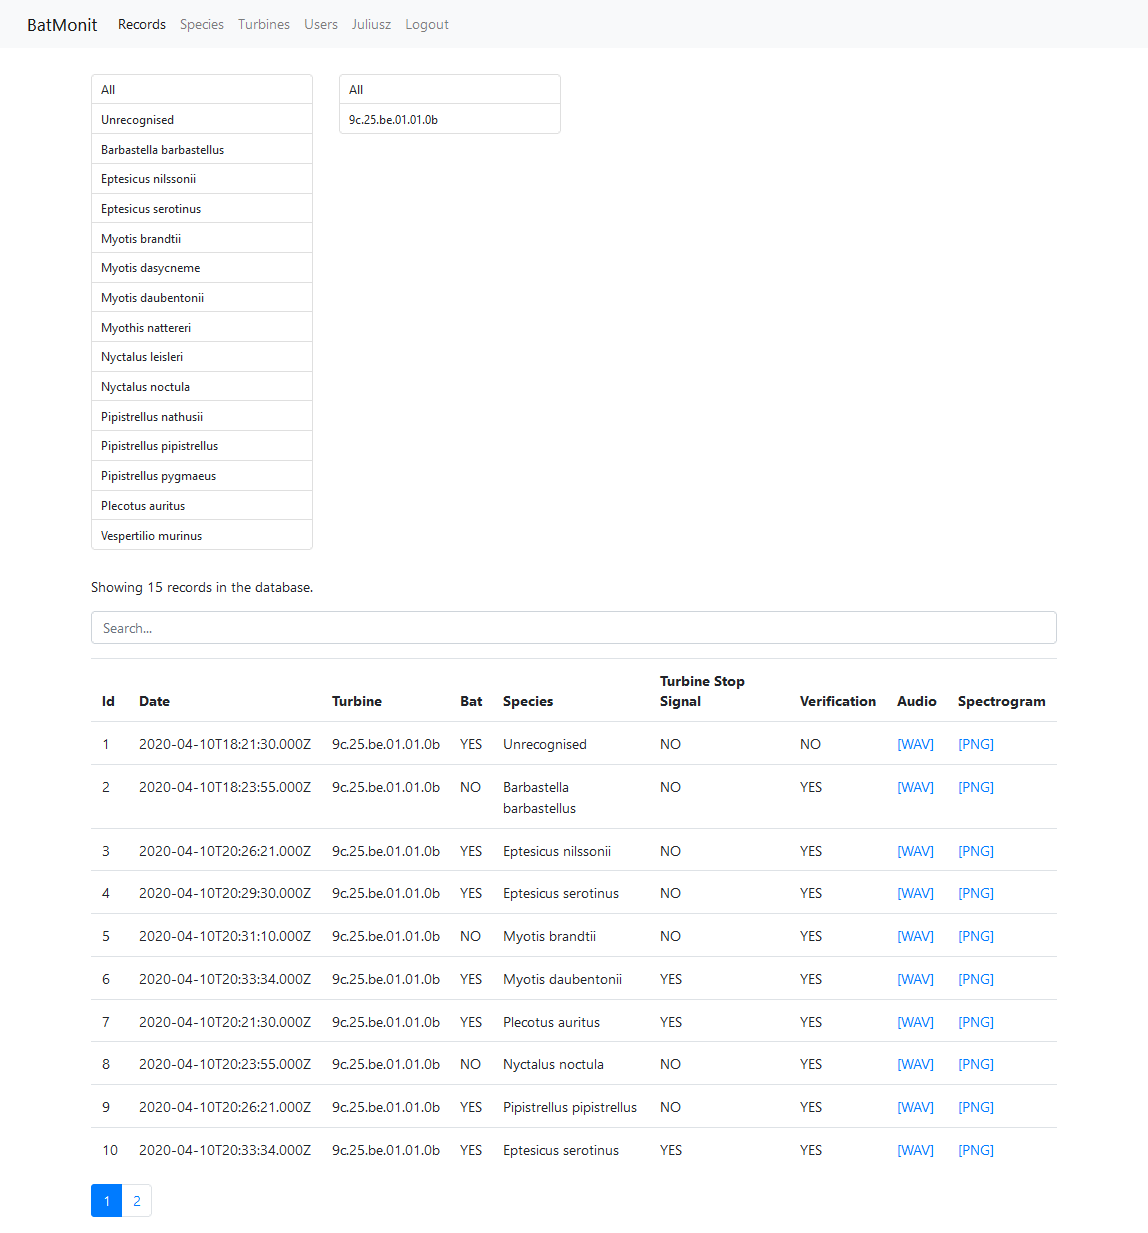
\includegraphics[width=0.8\textwidth]{sprz/app_records}
  \caption{Widok listy rekordów}
  \label{img:app_records}
\end{figure}

\chapter{Podsumowanie}

Praca nad rozwiązaniem objętym niniejszym dyplomem zbiegła się w czasie z dwoma istotnymi wydarzeniami, czy też procesami, które znacząco wpływają na przyszły kształt i możliwość komercjalizacji produktu. Były to: wprowadzenie na rynek przez firmę Wildlife Acoustics systemu SMART, który w części odpowiadał zakresowi pracy dyplomowej oraz gwałtowny rozwój sztucznej inteligencji i aplikacji jej w różnych dziedzinach życia, w tym w automatycznej identyfikacji nietoperzy.

W związku z wytworzeniem przez firmę Wildife Acoustics dość zaawansowanego rozwiązania jakim jest system SMART, można było albo wykorzystać to rozwiązanie i poprawić oraz dostosować funkcjonowanie niektórych jego elementów lub też skupić się na wytworzeniu autorskiego rozwiązania. Zarówno w trakcie konsultacji w Bioseco S.A. jak i konsultacji z prowadzącymi przedmioty związane z pracą dyplomową, zdecydowano się na wykorzystanie systemu SMART jako rozwiązania zdecydowanie szybszego w implementacji na farmach wiatrowych, co odpowiadało na potrzeby zarówno Klienta Zewnętrznego (Bioseco S.A. i klienci firmy) oczekującego szybkiego wdrożenia rozwiązania do ochrony nietoperzy, jak i Klienta Wewnętrznego (Dziekan, Promotor) wymagającego sprawnego ukończenia pracy dyplomowej.
Ponadto należy zauważyć, że firma Wildlife Acoustics posiada 20-letnie doświadczenie w konstrukcji mikrofonów ultradźwięków oraz jest autorem oprogramowania do automatycznej identyfikacji nietoperzy. Było to dodatkowym czynnikiem, który spowodował raczej wybór tego rozwiązania, niż rozpoczynanie podobnej drogi co firma Wildlife Acoustics i jej podobne wiele lat temu.

System SMART składa się z mikrofonu ultradźwięków i kontrolera będącego prostym komputerem przemysłowym, który serwuje aplikację udostępniającą dane z mikrofonu po uprzedniej odpowiedniej konfiguracji sieciowej. Taka dość zaawansowana konstrukcja rozwiązania spowodowała trudność dla mało doświadczonego zespołu inżynierskiego z ograniczonymi zasobami czasowymi w dotarciu do surowych danych płynących z mikrofonu. Z tego powodu wykorzystano nagrania, które zostały już zarejestrowane na kontrolerze i dopiero te dźwięki pobierano i poddawano analizie pod kątem gatunków nietoperzy i dalszej wizualizacji w aplikacji użytkownika. Prostota takiego rozwiązania odpowiadała zasadniczo celom i zakresowi pracy inżynierskiej, która nie miała doprowadzić do zaprojektowania rozwiązania gotowego do aplikacji na turbinach, a raczej jego prototyp. Rozwiązanie takie z uwagi na swą niegeneryczność, nie będzie stosowane w rozwiązaniu końcowym. Mimo to przynajmniej dwa elementy zrealizowane w ramach niniejszej pracy dyplomowej po dalszym dostosowaniu mają znaczny potencjał komercjalizacji. Do tych elementów należą bardziej zaawansowana pod kątem konstrukcyjnym aplikacja użytkownika w stosunku do aplikacji Wildlife Acoustics, zawierająca bazę danych oraz model sieci neuronowych z potencjałem do zwiększania dokładności identyfikacji gatunków nietoperzy, jednak po jego dalszym dopracowaniu. Aktualne poziomy dokładności identyfikacji nietoperzy przez tego typu oprogramowanie mieszczą się bowiem przykładowo w przedziałach: 28-82\% \cite{kaleidoscope-accuracy} czy 40-80\% \cite{kaleidoscope-bias}. Wykazuje się również, że nowsze oprogramowanie do automatycznej identyfikacji nie przynosi poprawy jeśli chodzi o dokładność oznaczeń. Jest to istotna nisza dla twórców niniejszej pracy dyplomowej z szansą na komercjalizację.

Dobrej jakości współpraca zapoczątkowana z firmą Wildlife Acoustics niesie możliwości kooperacji we wdrożeniu alternatywnych sposobów serwowania danych, w tym użycie własnego klasyfikatora. Sama firma umożliwia korzystanie z udostępnionych poleceń Linux w celu dostępu i autorskiej manipulacji danymi \cite{smart-linux-guide}.

Aplikacja serwowana przez kontroler, mimo wielu ciekawych i potrzebnych w kontekście wykorzystania systemu SMART na farmach wiatrowych funkcjonalności nie posiada bazy danych. Brak bazy danych wpływa m.in. na brak możliwości precyzyjnego filtrowania danych, w tym danych pobieranych poprzez aplikację do plików CSV, nie ma też łatwej możliwości przygotowania raportów z aktywności nietoperzy na farmie wiatrowej. Wykorzystanie w tym celu aplikacji, jaka została przygotowania w niniejszej pracy dyplomowej takich możliwości dostarcza. Jednak uprzednio aplikacja musiałaby być prawdopodobnie zintegrowana z aktualnym ekosystemem programistycznym firmy Bioseco S.A.. W obecnej postaci nie jest więc produktem gotowym do wdrożenia. Jednak z uwagi na zaznajomienie się twórców pracy z wieloma zagadnieniami związanymi z tworzeniem tego typu oprogramowania oraz zagadnieniami dziedzinowymi szansa na komercjalizację interfejsu użytkownika z bazą danych wytworzonymi w oparciu o system przygotowany w niniejszej pracy, jest bardzo wysoka. 

W niniejszej pracy dyplomowej udało się zrealizować wszystkie wymagania systemowe zdefiniowane w początkowej fazie przygotowania projektu poza oczekiwaną dokładnością sieci neuronowej. Jedno z wymagań zostało zaniechane w trakcie implementacji systemu i konsultacji z Bioseco S.A. i była nim implementacja zatrzymań turbiny wiatrowej, czego powody wyjaśniono w punkcie "Testy funkcjonalne" (System do zatrzymywania turbiny wiatrowej). 

Z sukcesem udało się zrozumieć całość tego interdyscyplinarnego problemu, który ma rozwiązywać zaprojektowany w pracy dyplomowej system oraz wytworzyć wszystkie jego komponenty. Nie udało się wytworzyć pobierania dźwięku z mikrofonu jako rozwiązania generycznego, czyli z wszystkimi elementami oprogramowania znajdującymi się na jednostce obliczeniowej zaimplementowanej przez zespół inżynierski. 

Udało się wdrożyć jedno z najnowocześniejszych podejść w automatycznej identyfikacji nietoperzy, jakim jest uczenie głębokie, które zaczęto stosować realnie dopiero na rok przed rozpoczęciem niniejszej pracy, a które daje bardzo dobre rezultaty w automatycznej identyfikacji gatunków nietoperzy. Niestety w niniejszej pracy nie udało się otrzymać zadowalających efektów, co mogło być spowodowane mało optymalnym przygotowaniem danych treningowych, np. braku odfiltrowania nagrań ze znajdującymi się dwoma gatunkami nietoperzy na jednym nagraniu.

Sukcesem jest z pewnością przezwyciężenie wszelkich trudności powstałych w trakcie trwania projektu, utrzymanie składu grupy inżynierskiej i skuteczna finalizacja pracy w zmiennych warunkach osobistych członków zespołu oraz przy złożeniu się niekorzystnych czynników losowych.

\chapter{Załączniki}

Na załączonej do niniejszej pracy płycie DVD znajdują się niżej wymienione dokumenty:
\begin{enumerate}
  \item Niniejsza praca w formacie PDF
  \item Dokument Założeń Wstępnych
  \item Specyfikacja Wymagań Systemowych
  \item Kod źródłowy oprogramowania i modelu
\end{enumerate}

\clearpage

\section{Diagram przypadków użycia}
\begin{figure}[h]
  \centering
  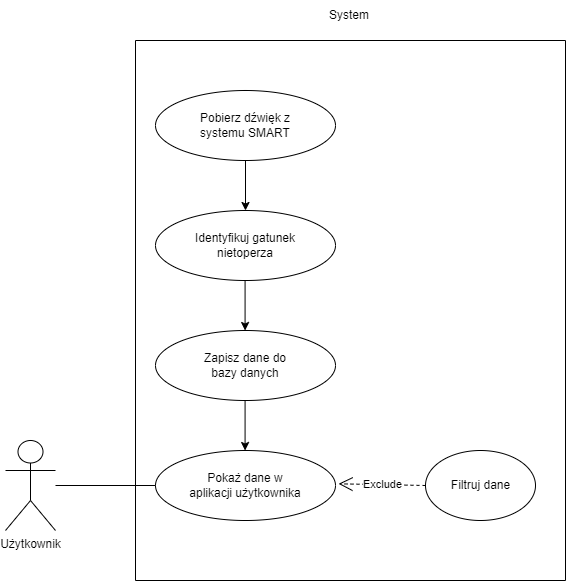
\includegraphics[width=0.9\textwidth]{sprz/use-case}
  \caption{Diagram przypadków użycia}
  \label{img:use-case}
\end{figure}

\printbibliography[title={Bibliografia}, heading=bibintoc]

\end{document}
